%%%%%%%%%%%%%%
%% Run LaTeX on this file several times to get Table of Contents,
%% cross-references, and citations.

%% If you have font problems, you may edit the w-bookps.sty file
%% to customize the font names to match those on your system.

%% w-bksamp.tex. Current Version: Feb 16, 2012
%%%%%%%%%%%%%%%%%%%%%%%%%%%%%%%%%%%%%%%%%%%%%%%%%%%%%%%%%%%%%%%%
%
%  Sample file for
%  Wiley Book Style, Design No.: SD 001B, 7x10
%  Wiley Book Style, Design No.: SD 004B, 6x9
%
%
%  Prepared by Amy Hendrickson, TeXnology Inc.
%  http://www.texnology.com
%%%%%%%%%%%%%%%%%%%%%%%%%%%%%%%%%%%%%%%%%%%%%%%%%%%%%%%%%%%%%%%%

%%%%%%%%%%%%%
% 7x10
%\documentclass{wileySev}

% 6x9
\documentclass{wileySix}

\usepackage{graphicx}

%%%%%%%
%% for times math: However, this package disables bold math (!)
%% \mathbf{x} will still work, but you will not have bold math
%% in section heads or chapter titles. If you don't use math
%% in those environments, mathptmx might be a good choice.

% \usepackage{mathptmx}

% For PostScript text
\usepackage{w-bookps}

%%%%%%%%%%%%%%%%%%%%%%%%%%%%%%%%%%%%%%%%%%%%%%%%%%%%%%%%%%%%%%%%
%% Other packages you might want to use:

% for chapter bibliography made with BibTeX
% \usepackage{chapterbib}

% for multiple indices
% \usepackage{multind}

% for answers to problems
% \usepackage{answers}

%%%%%%%%%%%%%%%%%%%%%%%%%%%%%%
%% Change options here if you want:
%%
%% How many levels of section head would you like numbered?
%% 0= no section numbers, 1= section, 2= subsection, 3= subsubsection
%%==>>
\setcounter{secnumdepth}{3}

%% How many levels of section head would you like to appear in the
%% Table of Contents?
%% 0= chapter titles, 1= section titles, 2= subsection titles, 
%% 3= subsubsection titles.
%%==>>
\setcounter{tocdepth}{2}

%% Cropmarks? good for final page makeup
%% \docropmarks

%%%%%%%%%%%%%%%%%%%%%%%%%%%%%%
%
% DRAFT
%
% Uncomment to get double spacing between lines, current date and time
% printed at bottom of page.
% \draft
% (If you want to keep tables from becoming double spaced also uncomment
% this):
% \renewcommand{\arraystretch}{0.6}
%%%%%%%%%%%%%%%%%%%%%%%%%%%%%%

%%%%%%% Demo of section head containing sample macro:
%% To get a macro to expand correctly in a section head, with upper and
%% lower case math, put the definition and set the box 
%% before \begin{document}, so that when it appears in the 
%% table of contents it will also work:

\newcommand{\VT}[1]{\ensuremath{{V_{T#1}}}}

%% use a box to expand the macro before we put it into the section head:

\newbox\sectsavebox
\setbox\sectsavebox=\hbox{\boldmath\VT{xyz}}

%%%%%%%%%%%%%%%%% End Demo


\begin{document}


\booktitle{Survey Methodology}
\subtitle{This is the Subtitle}

\authors{Robert M. Groves\\
\affil{Universitat de les Illes Balears}
Floyd J. Fowler, Jr.\\
\affil{University of New Mexico}
}

\offprintinfo{Survey Methodology, Second Edition}{Robert M. Groves}

%% Can use \\ if title, and edition are too wide, ie,
%% \offprintinfo{Survey Methodology,\\ Second Edition}{Robert M. Groves}

%%%%%%%%%%%%%%%%%%%%%%%%%%%%%%
%% 
\halftitlepage

\titlepage


\begin{copyrightpage}{2007}
Survey Methodology / Robert M. Groves . . . [et al.].
\       p. cm.---(Wiley series in survey methodology)
\    ``Wiley-Interscience."
\    Includes bibliographical references and index.
\    ISBN 0-471-48348-6 (pbk.)
\    1. Surveys---Methodology.  2. Social 
\  sciences---Research---Statistical methods.  I. Groves, Robert M.  II. %
Series.\\

HA31.2.S873 2007
001.4'33---dc22                                             2004044064
\end{copyrightpage}

\dedication{To my parents}

\begin{contributors}
\name{Masayki Abe,} Fujitsu Laboratories Ltd., Fujitsu Limited, Atsugi,
Japan

\name{L. A. Akers,} Center for Solid State Electronics Research, Arizona
State University, Tempe, Arizona

\name{G. H. Bernstein,} Department of Electrical and
Computer Engineering, University of Notre Dame, Notre Dame, South Bend, 
Indiana; formerly of
Center for Solid State Electronics Research, Arizona
State University, Tempe, Arizona 
\end{contributors}

\contentsinbrief
\tableofcontents
\listoffigures
\listoftables


\begin{foreword}
This is the foreword to the book.
\end{foreword}

\begin{preface}
This is an example preface.
This is an example preface.
This is an example preface.
This is an example preface.

\prefaceauthor{R. K. Watts}
\where{Durham, North Carolina\\
September, 2007}

\end{preface}


\begin{acknowledgments}
From Dr.~Jay Young, consultant from Silver Spring, Maryland, I received
the initial push to even consider writing this book. Jay was a constant
``peer reader'' and very welcome advisor durying this year-long process.


To all these wonderful people I owe a deep sense of gratitude especially now
that this project has been completed.
\authorinitials{G. T. S.}
\end{acknowledgments}

\begin{acronyms}
\acro{ACGIH}{American Conference of Governmental Industrial Hygienists}
\acro{AEC}{Atomic Energy Commission}
\acro{OSHA}{Occupational Health and Safety Commission}
\acro{SAMA}{Scientific Apparatus Makers Association}
\end{acronyms}

\begin{glossary}
\term{NormGibbs}Draw a sample from a posterior distribution
of data with an unknown mean and variance using Gibbs sampling.

\term{pNull}Test a one sided hypothesis from a numberically
specified posterior CDF or from a sample from the posterior

\term{sintegral}A numerical integration using Simpson's rule
\end{glossary}

\begin{symbols}
\term{A}Amplitude

\term{\hbox{\&}}Propositional logic symbol 

\term{a}Filter Coefficient

\bigskip

\term{\mathcal{B}}Number of Beats
\end{symbols}

\begin{introduction}

%% optional, but if you want to list author:

\introauthor{Catherine Clark, PhD.}
{Harvard School of Public Health\\
Boston, MA, USA}

The era of modern \index{microelectronics}\index{microelectronics!modern} 
began in 1958 with the invention of the
integrated circuit by J.~S.~Kilby
 of Texas Instruments \cite{kilby}.
His first chip is shown in Fig.~I. For comparison,
Fig.~I.2 shows a modern microprocessor chip, \cite{beren}.


This is the introduction.
This is the introduction.
This is the introduction.
This is the introduction.
This is the introduction.
This is the introduction.

\begin{equation}
ABC {\cal DEF} \alpha\beta\Gamma\Delta\sum^{abc}_{def}
\end{equation}


\begin{chapreferences}{3.}
\bibitem{zkilby}J. S. Kilby,
``Invention of the Integrated Circuit,'' {\it IEEE Trans. Electron Devices,}
{\bf ED-23,} 648 (1976).

\bibitem{zhamming}R. W. Hamming,
                 {\it Numerical Methods for Scientists and 
                 Engineers}, Chapter N-1, McGraw-Hill, 
                 New York, 1962.

\bibitem{zHu}J. Lee, K. Mayaram, and C. Hu, ``A Theoretical
               Study of Gate/Drain Offset in LDD MOSFETs''
                     {\it IEEE Electron Device Lett.,} {\bf EDL-7}(3). 152 
                     (1986).
\end{chapreferences}
\end{introduction}

\chapter{Home}

\chapter{Basic Concept}

\chapter{Environtment Setup}

\chapter{Life Cycle}

\chapter{Create Operation}

\sloppy
{\fontsize{14pt}{14pt}\selectfont CREAT OPRATION \\} \par
\vspace{14pt}
\noindent 
{\fontsize{14pt}{14pt}\selectfont Dasar Git \\} \par
\noindent 
{\fontsize{14pt}{14pt}\selectfont Jadi, sebenarnya apa yang dimaksud dengan Git? Ini adalah bagian penting untuk dipahami, karena jika anda memahami apa itu Git dan cara kerjanya, maka dapat dipastikan anda dapat menggunakan Git secara efektif dengan mudah. Selama mempelajari Git, cobalah untuk melupakan VCS lain yang mungkin telah anda kenal sebelumnya, misalnya Subversion dan Perforce. Git sangat berbeda dengan sistem-sistem tersebut dalam hal menyimpan dan memperlakukan informasi yang digunakan, walaupun antar-muka penggunanya hampir mirip. Dengan memahami perbedaan tersebut diharapkan dapat membantu anda menghindari kebingungan saat menggunakan Git. \\} \par

 \par
\noindent 
{\fontsize{14pt}{14pt}\selectfont Salah satu perbedaan yang mencolok antar Git dengan VCS lainnya (Subversion dan kawan-kawan) adalah dalam cara Git memperlakukan datanya. Secara konseptual, kebanyakan sistem lain menyimpan informasi sebagai sebuah daftar perubahan berkas. Sistem seperti ini (CVS, Subversion, Bazaar, dan yang lainnya) memperlakukan informasi yang disimpannya sebagai sekumpulan berkas dan perubahan yang terjadi pada berkas-berkas tersebut, \\} \par
\vspace{14pt}
\noindent 
{\fontsize{14pt}{14pt}\selectfont Git tidak bekerja seperti ini. Melainkan, Git memperlakukan datanya sebagai sebuah kumpulan snapshot dari sebuah miniatur sistem berkas. Setiap kali anda melakukan commit, atau melakukan perubahan pada proyek Git anda, pada dasarnya Git merekam gambaran keadaan berkas-berkas anda pada saat itu dan menyimpan referensi untuk gambaran tersebut. Agar efisien, jika berkas tidak mengalami perubahan, Git tidak akan menyimpan berkas tersebut melainkan hanya pada file yang sama yang sebelumnya telah disimpan. \\} \par
\vspace{14pt}
\noindent 
{\fontsize{14pt}{14pt}\selectfont erbedaan penting antara Git dengan hampir semua VCS lain. Hal ini membuat Git mempertimbangkan kembali hampir setiap aspek dari version control yang oleh kebanyakan sistem lainnya disalin dari generasi sebelumnya. Ini membuat Git lebih seperti sebuah miniatur sistem berkas dengan beberapa tool yang luar biasa ampuh yang dibangun di atasnya, ketimbang sekadar sebuah VCS. $  $ \\} \par

 \par
\noindent 
{\fontsize{14pt}{14pt}\selectfont Kebanyakan operasi pada Git hanya membutuhkan berkas-berkas dan resource lokal – tidak ada informasi yang dibutuhkan dari komputer lain pada jaringan anda. Jika Anda terbiasa dengan VCS terpusat dimana kebanyakan operasi memiliki overhead latensi jaringan, aspek Git satu ini akan membuat anda berpikir bahwa para dewa kecepatan telah memberkati Git dengan kekuatan. Karena anda memiliki seluruh sejarah dari proyek di lokal disk anda, dengan kebanyakan operasi yang tampak hampir seketika. \\} \par
\noindent 
{\fontsize{14pt}{14pt}\selectfont Sebagai contoh, untuk melihat history dari proyek, Git tidak membutuhkan data histori dari server untuk kemudian menampilkannya untuk anda, namun secara sedarhana Git membaca historinya langsung dari basisdata lokal proyek tersebut. Ini berarti anda melihat histori proyek hampir secara instant. Jika anda ingin membandingkan perubahan pada sebuah berkas antara versi saat ini dengan versi sebulan yang lalu, Git dapat mencari berkas yang sama pada sebulan yang lalu dan melakukan pembandingan perubahan secara lokal, bukan dengan cara meminta remote server melakukannya atau meminta server mengirimkan berkas versi yang lebih lama kemudian membandingkannya secara lokal. \\} \par
\noindent 
{\fontsize{14pt}{14pt}\selectfont Hal ini berarti bahwa sangat sedikit yang tidak bisa anda kerjakan jika anda sedang offline atau berada diluar VPN. Jika anda sedang berada dalam pesawat terbang atau sebuah kereta dan ingin melakukan pekerjaan kecil, anda dapat melakukan commit sampai anda memperoleh koneksi internet hingga anda dapat menguploadnya. Jika anda pulang ke rumah dan VPN client anda tidak bekerja dengan benar, anda tetap dapat bekerja. Pada kebanyakan sistem lainnya, melakukan hal ini cukup sulit atau bahkan tidak mungkin sama sekali. Pada Perforce misalnya, anda tidak dapat berbuat banyak ketika anda tidak terhubung dengan server; pada Subversion dan CVS, anda dapat mengubah berkas, tapi anda tidak dapat melakukan commit pada basisdata anda (karena anda tidak terhubung dengan basisdata). Hal ini mungkin saja bukanlah masalah yang besar, namun anda akan terkejut dengan perbedaan besar yang disebabkannya. \\} \par

 \par
\noindent 
{\fontsize{14pt}{14pt}\selectfont Segala sesuatu pada Git akan melalui proses checksum terlebih dahulu sebelum disimpan yang kemudian direferensikan oleh hasil checksum tersebut. Hal ini berarti tidak mungkin melakukan perubahan terhadap berkas manapun tanpa diketahui oleh Git. Fungsionalitas ini dimiliki oleh Git pada level terendahnya dan ini merupakan bagian tak terpisahkan dari filosofi Git. Anda tidak akan kehilangan informasi atau mendapatkan file yang cacat tanpa diketahui oleh Git. \\} \par
\vspace{14pt}
\vspace{14pt}
\vspace{12pt}
\vspace{12pt}
\noindent 
{\fontsize{14pt}{14pt}\selectfont \underline{Secara Umum Git Hanya Menambahkan Data} \\} \par
\noindent 
{\fontsize{14pt}{14pt}\selectfont Ketika anda melakukan operasi pada Git, kebanyakan dari operasi tersebut hanya menambahkan data pada basisdata Git. It is very difficult to get the system to do anything that is not undoable or to make it erase data in any way. Seperti pada berbagai VCS, anda dapat kehilangan atau mengacaukan perubahan yang belum di-commit; namun jika anda melakukan commit pada Git, akan sangat sulit kehilanngannya, terutama jika anda secara teratur melakukan push basisdata anda pada repositori lain. \\} \par
\noindent 
{\fontsize{14pt}{14pt}\selectfont Hal ini menjadikan Git menyenangkan karena kita dapat berexperimen tanpa kehawatiran untuk mengacaukan proyek. Untuk lebih jelas dan dalam lagi tentang bagaimana Git menyimpan datanya dan bagaimana anda dapat mengembalikan yang hilang, lihat "Under the Covers" pada Bab 9. \\} \par

 \par
\noindent 
{\fontsize{14pt}{14pt}\selectfont Sekarang perhatikan. Ini adalah hal utama yang harus diingat tentang Git jika anda ingin proses belajar anda berjalan lancar. Git memiliki 3 keadaan utama dimana berkas anda dapat berada: committed, modified dan staged. Committed berarti data telah tersimpan secara aman pada basisdata lokal. Modified berarti anda telah melakukan perubahan pada berkas namun anda belum melakukan commit pada basisdata. Staged berarti anda telah menandai berkas yang telah diubah pada versi yang sedang berlangsung untuk kemudian dilakukan commit. \\} \par
\vspace{14pt}
\vspace{14pt}
\noindent 
{\fontsize{14pt}{14pt}\selectfont Direktori Git adalah dimana Git menyimpan metadata dan database objek untuk projek anda. Ini adalah bahagian terpenting dari Git, dan inilah yang disalin ketika anda melakukan kloning sebuah repository dari komputer lain. \\} \par
\noindent 
{\fontsize{14pt}{14pt}\selectfont Direktori kerja adalah sebuah checkout tunggal dari satu versi dari projek. Berkas-berkas ini kemudian ditarik keluar dari basisdata yang terkompresi dalam direktori Git dan disimpan pada disk untuk anda gunakan atau modifikasi. \\} \par
\noindent 
{\fontsize{14pt}{14pt}\selectfont Staging area adalah sebuah berkas sederhana, umumnya berada dalam direktori Git anda, yang menyimpan informasi mengenai apa yang menjadi commit selanjutnya. Ini terkadang disebut sebagai index, tetapi semakin menjadi standard untuk menyebutnya sebagai staging area. \\} \par
\noindent 
{\fontsize{14pt}{14pt}\selectfont Alur kerja dasar Git adalah seperti ini: \\} \par
\noindent 
{\fontsize{14pt}{14pt}\selectfont Anda mengubah berkas dalam direktori kerja anda. \\} \par
\noindent 
{\fontsize{14pt}{14pt}\selectfont Anda membawa berkas ke stage, menambahkan snapshotnya ke staging area. \\} \par
\noindent 
{\fontsize{14pt}{14pt}\selectfont Anda melakukan commit, yang mengambil berkas seperti yang ada di staging area dan menyimpan snapshotnya secara permanen ke direktori Git anda. \\} \par
\noindent 
{\fontsize{14pt}{14pt}\selectfont Jika sebuah versi tertentu dari sebuah berkas telah ada di direktori git, ia dianggap 'committed'. Jika berkas diubah (modified) tetapi sudah ditambahkan ke staging area, maka itu adalah 'staged'. Dan jika berkas telah diubah sejak terakhir dilakukan checked out tetapi belum ditambahkan ke staging area maka itu adalah 'modified' \\} \par
\vspace{14pt}
\vspace{14pt}
\noindent 
{\fontsize{14pt}{14pt}\selectfont Mari memulai menggunakan Git. Pertama, tentu saja anda harus menginstallnya terlebih dahulu. Anda dapat melakukan melalui berbagai cara; dua cara paling poluler adalah menginstallnya dari kode sumbernya atau menginstalkan paket yang telah disediakan untuk platform anda. \\} \par

 \par
\noindent 
{\fontsize{14pt}{14pt}\selectfont Jika anda dapat melakukannya, akan sangat berguna untuk dapat menginstallnya dari kode sumber, karena anda akan mendapatkan versi terbaru dari Git. Setiap versi dari Git cenderung akan menampilkan kemajuan pada sisi antarmuka pengguna, jadi menggunakan versi terbaru seringkali menjadi jalan terbaik jika anda terbiasa melakukan kompilasi perangkat lunak dari kode sumbernya. Dan juga menjadi masalah bahwa banyak distribusi Linux yang menyertakan versi Git yang sangat lama; kecuali anda mempergunakan distribusi Linux paling up-to-date atau menggunakan backport, menginstall dari kode sumbernya mungkin menjadi solusi terbaik. \\} \par
\vspace{14pt}
\noindent 
{\fontsize{14pt}{14pt}\selectfont Setup Git Untuk Pertama Kalinya \\} \par
\noindent 
{\fontsize{14pt}{14pt}\selectfont Sekarang anda telah memiliki Git pada sistem anda, berikutnya anda akan harus melakukan beberapa penyesuai pada lingkungan Git anda. Anda hanya perlu melakukan hal ini sekali saja; pada saat memperbaharui versi Git anda, penyesuai tidak perlu dilakukan lagi. Anda pun dapat mengubah penyesuaian tersebut setiap saat. \\} \par
\noindent 
{\fontsize{14pt}{14pt}\selectfont Pada Git terdapat sebuah perkakas yang disebut dengan git config yang memungkinkan anda untuk memperoleh informasi dan menetapkan variable konfigurasi yang mengontrol segala aspek bagaimana Git beroperasi dan berperilaku. Variable-variable ini dapat disimpan pada tiga tempat berbeda: gitconfig $  $file: Menyimpan berbagai nilai-nilai variable untuk setiap pengguna pada sistem dan semua repositori milik para pengguna tersebut. Jika anda memberikan opsi $  $--system $  $pada $  $git config, maka Git akan membaca dan menulis file konfigurasi ini secara spesifik. gitconfig $  $file: Spesifik hanya untuk pengguna yang bersangkutan. Anda dapat membuat Git membaca dan menulis pada berkas ini secara spesifik dengan memberikan opsi $  $--global. \\} \par
\noindent 
{\fontsize{14pt}{14pt}\selectfont config file pada direktori git (yaitu, $  $.git config) atau reposotori manapun yang sedang anda gunakan: Spesifik hanya pada repositori itu saja. Setiap nilai pada setiap tingkat akan selalu menimpa nilai yang telah ditetapkan pada level sebelumnya, jadi nilai yang telah di-set pada $  $.git configakan menimpa nilai yang telah di-set pada $  $gitconfig. \\} \par
\vspace{14pt}
\noindent 
{\fontsize{14pt}{14pt}\selectfont Apakah Branch Itu \\} \par
\noindent 
{\fontsize{14pt}{14pt}\selectfont Untuk benar-benar mengerti cara Git melakukan branching, kita perlu kembali ke belakang dan membahas bagaimana Git menyimpan datanya. Seperti yang mungkin anda ingat dari Bab 1, Git tidak menyimpan data sebagai serangkaian kumpulan perubahan atau delta, melainkan sebagai serangkaian snapshot. \\} \par
\noindent 
{\fontsize{14pt}{14pt}\selectfont Ketika anda melakukan commit dalam Git, Git menyimpan sebuah object commit yang berisi pointer ke snapshot dari konten yang anda staged, metadata pembuat (author) dan pesan (message), dan nol atau lebih pointer ke commit yang merupakan parent (induk) langsung dari commit ini: nol jika ini commit yang pertama, satu jika ini commit yang normal, dan beberapa jika ini commit yang dihasilkan dari gabungan antara dua atau lebih branch. \\} \par
\noindent 
{\fontsize{14pt}{14pt}\selectfont Untuk memvisualisasikan ini, mari kita asumsikan anda memiliki direktori yang berisi tiga buah berkas, dan anda menambahkan mereka ke stage dan melakukan commit. Proses staging berkas melakukan checksum (dengan hash SHA-1 yang telah kita sebutkan di Bab 1), menyimpan versi berkas tersebut dalam repositori Git (Git merujuknya sebagai 'blobs') \\} \par
\noindent 
{\fontsize{14pt}{14pt}\selectfont Apa itu version control, dan kenapa anda harus peduli? Version control adalah sebuah sistem yang mencatat setiap perubahan terhadap sebuah berkas atau kumpulan berkas sehingga pada suatu saat anda dapat kembali kepada salah satu versi dari berkas tersebut. Sebagai contoh dalam buku ini anda akan menggunakan kode sumber perangkat lunak sebagai berkas yang akan dilakukan version controlling, meskipun pada kenyataannya anda dapat melakukan ini pada hampir semua tipe berkas di komputer. \\} \par
\noindent 
{\fontsize{14pt}{14pt}\selectfont Jika anda adalah seorang desainer grafis atau desainer web dan anda ingin menyimpan setiap versi dari gambar atau layout yang anda buat (kemungkinan besar anda pasti ingin melakukannya), maka Version Control System (VCS) merupakan sebuah solusi bijak untuk digunakan. Sistem ini memungkinkan anda untuk mengembalikan berkas anda pada kondisi/keadaan sebelumnya, mengembalikan seluruh proyek pada keadaan sebelumnya, membandingkan perubahan setiap saat, melihat siapa yang terakhir melakukan perubahan terbaru pada suatu objek sehingga berpotensi menimbulkan masalah, siapa yang menerbitkan isu, dan lainnya. Dengan menggunakan VCS dapat berarti jika anda telah mengacaukan atau kehilangan berkas, anda dapat dengan mudah mengembalikannya. Ditambah lagi, anda mendapatkan semua ini dengan overhead yang sangat sedikit. \\} \par

 \par
\noindent 
{\fontsize{14pt}{14pt}\selectfont Kebanyakan orang melakukan pengontrolan versi dengan cara menyalin berkas-berkas pada direktori lain (mungkin dengan memberikan penanggalan pada direktori tersebut, jika mereka rajin). Metode seperti ini sangat umum karena sangat sederhana, namun cenderung rawan terhadap kesalahan. Anda akan sangat mudah lupa dimana direktori anda sedang berada, selain itu dapat pula terjadi ketidak sengajaan penulisan pada berkas yang salah atau menyalin pada berkas yang bukan anda maksudkan. \\} \par
\noindent 
{\fontsize{14pt}{14pt}\selectfont Untuk mengatasi permasalahan ini, para programmer mengembangkan berbagai VCS lokal yang memiliki sebuah basis data sederhana untuk menyimpan semua perubahan pada berkas yang berada dalam cakupan revision control \\} \par
\vspace{14pt}
\noindent 
{\fontsize{14pt}{14pt}\selectfont Mengambil Repositori Git \\} \par
\noindent 
{\fontsize{14pt}{14pt}\selectfont Anda dapat mengambil sebuah proyek Git melalui 2 pendekatan utama. Cara pertama adalah dengan mengambil proyek atau direktori tersedia untuk dimasukkan ke dalam Git. Cara kedua adalah dengan melakukan kloning/duplikasi dari repositori Git yang sudah ada dari server. \\} \par

 \par
\noindent 
{\fontsize{14pt}{14pt}\selectfont Jika Anda mulai memantau proyek yang sudah ada menggunakan Git, Anda perlu masuk ke direktori dari proyek tersebut dan mengetikkan \\} \par
\noindent 
{\fontsize{14pt}{14pt}\selectfont  $  \$  $ git init \\} \par
\noindent 
{\fontsize{14pt}{14pt}\selectfont Git akan membuat sebuah subdirektori baru bernama .git yang akan berisi semua berkas penting dari repositori Anda, yaitu kerangka repositori dari Git. Pada titik ini, belum ada apapun dari proyek Anda yang dipantau. (Lihat Bab 9 untuk informasi lebih lanjut mengenai berkas apa saja yang terdapat di dalam direktori $  $.git $  $yang baru saja kita buat.) \\} \par
\noindent 
{\fontsize{14pt}{14pt}\selectfont Jika Anda ingin mulai mengendalikan versi dari berkas tersedia (bukan direktori kosong), Anda lebih baik mulai memantau berkas tersebut dengan melakukan commit awal. Caranya adalah dengan beberapa perintah $  $git add $  $untuk merumuskan berkas yang ingin anda pantau, diikuti dengan sebuah commit: \\} \par
\noindent 
{\fontsize{14pt}{14pt}\selectfont git add *.c \\} \par
\noindent 
{\fontsize{14pt}{14pt}\selectfont git add README \\} \par
\noindent 
{\fontsize{14pt}{14pt}\selectfont it commit –m 'versi awal proyek' \\} \par
\noindent 
{\fontsize{14pt}{14pt}\selectfont Kita akan membahas apa yang dilakukan perintah-perintah di atas sebentar lagi. Pada saat ini, Anda sudah memiliki sebuah repositori Git berisi file-file terpantau dan sebuah commit awal. \\} \par

 \par
\noindent 
{\fontsize{14pt}{14pt}\selectfont Jika Anda ingin membuat salinan dari repositori Git yang sudah tersedia — misalnya, dari sebuah proyek yang Anda ingin ikut berkontribusi di dalamnya — perintah yang Anda butuhkan adalah $  $git clone. Jika Anda sudah terbiasa dengan sistem VCS lainnya seperti Subversion, Anda akan tersadar bahwa perintahnya adalah clone dan bukan checkout. Ini adalah pembedaan yang penting — Git menerima salinan dari hampir semua data yang server miliki. Setiap versi dari setiap berkas yang tercatat dalam sejarah dari proyek tersebut akan ditarik ketika Anda menjalankan $  $git clone. Bahkan, ketika cakram di server Anda rusak, Anda masih dapat menggunakan hasil duplikasi di klien untuk mengembalikan server Anda ke keadaan tepat pada saat duplikasi dibuat (Anda mungkin kehilangan beberapa hooks atau sejenisnya yang sebelumnya telah ditata di sisi server, namun semua versi data sudah kembali seperti sediakala-lihat Bab 4 untuk lebih detil). \\} \par
\noindent 
{\fontsize{14pt}{14pt}\selectfont Anda menduplikasi sebuah repositori menggunakan perintah $  $git clone [url]. Sebagai contoh, jika Anda ingin menduplikasi pustaka Git Ruby yang disebut Grit, Anda dapat melakukannya sebagai berikut: \\} \par
\noindent 
{\fontsize{14pt}{14pt}\selectfont git clone git://github.com/schacon/grit.git \\} \par
\noindent 
{\fontsize{14pt}{14pt}\selectfont Perintah ini akan membuat sebuah direktori yang dinamakan "grit", menata awal sebuah direktori $  $.gitdi dalamnya, menarik semua data dari repositori, dan $  $checkout $  $versi mutakhir dari salinan kerja. Jika Anda masuk ke dalam direktori $  $grit $  $tersebut, Anda akan melihat berkas-berkas proyek sudah ada di sana, siap untuk digunakan. Jika Anda ingin membuat duplikasi dari repositori tersebut ke direktori yang tidak dinamakan grit. \\} \par
\noindent 
{\fontsize{14pt}{14pt}\selectfont Perintah ini bekerja seperti perintah sebelumnya, namun direktori tujuannya akan diberi nama mygrit. \\} \par
\noindent 
{\fontsize{14pt}{14pt}\selectfont Git memiliki beberapa protokol transfer yang berbeda yang dapat digunakan. Pada contoh sebelumnya, kita menggunakan protokol $  $ yang akan menggunakan SSH sebagai protokol transfer. Bab 4 akan memperkenalkan Anda kepada semua opsi yang tersedia yang dapat ditata di sisi server untuk mengakses repositori Git Anda dan keuntungan dan kelebihan dari masing-masing protokol. \\} \par
\vspace{14pt}
\noindent 
{\fontsize{14pt}{14pt}\selectfont Jika Anda hanya sempat membaca satu bab untuk dapat bekerja dengan Git, bab inilah yang tepat. Bab ini menjelaskan setiap perintah dasar yang Anda butuhkan untuk menyelesaikan sebagian besar permasalahan yang akan Anda hadapi dalam penggunaan Git. Pada akhir bab, Anda akan dapat mengkonfigurasi dan memulai sebuah repositori, memulai dan mengakhiri pemantauan berkas, dan melakukan staging dan committing perubahannya. Kami juga akan menunjukkan kepada Anda cara menata Git untuk mengabaikan berkas-berkas ataupun pola berkas tertentu, cara untuk membatalkan kesalahan secara cepat dan mudah, cara untuk melihat sejarah perubahan dari proyek dan melihat perubahan-perubahan yang telah terjadi diantara commit, dan cara untuk mendorong dan menarik perubahan dari repositori lain. \\} \par
\vspace{14pt}
\noindent 
{\fontsize{14pt}{14pt}\selectfont Merekam Perubahan ke dalam Repositori \\} \par
\noindent 
{\fontsize{14pt}{14pt}\selectfont Anda sudah memiliki repositori Git yang bonafide dan sebuah salinan kerja dari semua berkas untuk proyek tersebut. Anda harus membuat beberapa perubahan dan commit perubahan tersebut ke dalam repositori setiap saat proyek mencapai sebuah keadaan yang ingin Anda rekam. \\} \par
\noindent 
{\fontsize{14pt}{14pt}\selectfont Ingat bahwa setiap berkas di dalam direktori kerja Anda dapat berada di 2 keadaan: terpantau atau tak-terpantau. Berkas terpantau adalah berkas yang sebelumnya berada di snapshot terakhir; mereka dapat berada dalam kondisi belum terubah, terubah, ataupun staged (berada di area stage). Berkas tak-terpantau adalah kebalikannya - merupakan berkas-berkas di dalam direktori kerja yang tidak berada di dalam snapshot terakhir dan juga tidak berada di area staging. Ketika Anda pertama kali menduplikasi sebuah repositori, semua berkas Anda akan terpantau dan belum terubah karena Anda baru saja melakukan checkout dan belum mengubah apapun. \\} \par

 \par
\noindent 
{\fontsize{14pt}{14pt}\selectfont Alat utama yang Anda gunakan untuk menentukan berkas-berkas mana yang berada dalam keadaan tertentu adalah melalui perintah $  $git status. Jika Anda menggunakan alat ini langsung setelah sebuah $  $clone, Anda akan melihat serupa seperti di bawah ini: \\} \par
\noindent 
{\fontsize{14pt}{14pt}\selectfont git status \\} \par
\noindent 
{\fontsize{14pt}{14pt}\selectfont On branch master \\} \par
\noindent 
{\fontsize{14pt}{14pt}\selectfont nothing to commit, working directory clean \\} \par
\noindent 
{\fontsize{14pt}{14pt}\selectfont Ini berarti Anda memiliki direktori kerja yang bersih-dengan kata lain, tidak ada berkas terpantau yang terubah. Git juga tidak melihat berkas-berkas yang tak terpantau, karena pasti akan dilaporkan oleh alat ini. Juga, perintah ini memberitahu Anda tentang cabang tempat Anda berada. Pada saat ini, cabang akan selalu berada di master, karena sudah menjadi default-nya; Anda tidak perlu khawatir tentang cabang dulu. Bab berikutnya akan membahas tentang percabangan dan referensi secara lebih detil. \\} \par

 \par
\noindent 
{\fontsize{14pt}{14pt}\selectfont Untuk mulai memantau berkas baru, Anda menggunakan perintah $  $git add. Untuk mulai memantau berkas README tadi, Anda menjalankannya seperti berikut: \\} \par
\noindent 
{\fontsize{14pt}{14pt}\selectfont git add README \\} \par
\noindent 
{\fontsize{14pt}{14pt}\selectfont Jika Anda menjalankan perintah $  $status $  $lagi, Anda akan melihat bahwa berkas README Anda sekarang sudah terpantau dan sudah masuk ke dalam area stage: \\} \par
\noindent 
{\fontsize{14pt}{14pt}\selectfont git status \\} \par
\noindent 
{\fontsize{14pt}{14pt}\selectfont On branch master \\} \par
\noindent 
{\fontsize{14pt}{14pt}\selectfont Changes to be committed: \\} \par
\noindent 
{\fontsize{14pt}{14pt}\selectfont use git reset HEAD <file>... to unstage \\} \par
\noindent 
{\fontsize{14pt}{14pt}\selectfont new~file:~  README \\} \par
\noindent 
{\fontsize{14pt}{14pt}\selectfont Anda dapat mengatakan bahwa berkas tersebut berada di dalam area stage karena tertulis di bawah judul Changes to be committed. Jika Anda melakukan commit pada saat ini, versi berkas pada saat Anda menjalankan $  $git add $  $inilah yang akan dimasukkan ke dalam sejarah snapshot. Anda mungkin ingat bahwa ketika Anda menjalankan $  $git init $  $sebelumnya, Anda melanjutkannya dengan $  $git add (nama berkas) $  $yang akan mulai dipantau di direktori Anda. Perintah $  $git add $  $ini mengambil alamat dari berkas ataupun direktori; jika sebuah direktori, perintah tersebut akan menambahkan seluruh berkas yang berada di dalam direktori secara rekursif. \\} \par
\vspace{14pt}
\vspace{14pt}
\noindent 
{\fontsize{14pt}{14pt}\selectfont Bekerja Berjarak \\} \par
\noindent 
{\fontsize{14pt}{14pt}\selectfont Untuk dapat berkolaborasi untuk proyek Git apapun, Anda perlu mengetahui bagaimana Anda dapat mengatur repositori berjarak dari jarak jauh. Repositori berjarak adalah sekumpulan versi dari proyek Anda yang disiarkan di Internet atau di jaringan. Anda dapat memiliki beberapa repositori berjarak, masing-masing bisanya dengan akses terbatas untuk membaca saja ataupun baca/tulis. Berkolaborasi dengan pihak lain menuntut kemampuan untuk mengatur repositori berjarak ini dan menarik dan mendorong data ke dan dari repositori berjarak tersebut ketika Anda butuh untuk membagi hasil kerja Anda. \\} \par
\vspace{14pt}
\noindent 
{\fontsize{14pt}{14pt}\selectfont Apakah Branch Itu \\} \par
\noindent 
{\fontsize{14pt}{14pt}\selectfont Untuk benar-benar mengerti cara Git melakukan branching, kita perlu kembali ke belakang dan membahas bagaimana Git menyimpan datanya. Seperti yang mungkin anda ingat dari Bab 1, Git tidak menyimpan data sebagai serangkaian kumpulan perubahan atau delta, melainkan sebagai serangkaian snapshot. \\} \par
\noindent 
{\fontsize{14pt}{14pt}\selectfont Ketika anda melakukan commit dalam Git, Git menyimpan sebuah object commit yang berisi pointer ke snapshot dari konten yang anda staged, metadata pembuat (author) dan pesan (message), dan nol atau lebih pointer ke commit yang merupakan parent (induk) langsung dari commit ini: nol jika ini commit yang pertama, satu jika ini commit yang normal, dan beberapa jika ini commit yang dihasilkan dari gabungan antara dua atau lebih branch. \\} \par
\vspace{14pt}
\noindent 
{\fontsize{14pt}{14pt}\selectfont Hampir setiap VCS memiliki sejumlah dukungan atas branching (percabangan). Branching adalah membuat cabang dari repositori utama dan melanjutkan melakukan pekerjaan pada cabang yang baru tersebut tanpa perlu khawatir mengacaukan yang utama. Dalam banyak VCS, branching adalah proses yang agak mahal, karena seringkali mengharuskan anda untuk membuat salinan baru dari direktori kode sumber, dimana dapat memakan waktu lama untuk proyek-proyek yang besar. \\} \par
\noindent 
{\fontsize{14pt}{14pt}\selectfont Beberapa orang menyebut model branching dalam Git sebagai "killer feature," hal inilah yang membuat Git berbeda di komunitas VCS. Mengapa begitu istimewa? Cara Git membuat cabang sangatlah ringan, membuat operasi branching hampir seketika dan berpindah bolak-balik antara cabang umumnya sama cepatnya. Tidak seperti VCS lainnya, Git mendorong alur kerja dimana kita sering membuat cabang dan kemudian menggabungkannya, bahkan dapat beberapa kali dalam sehari. Memahami dan menguasai fitur ini memberi anda perangkat yang ampuh, unik, dan benar-benar dapat mengubah cara anda melakukan pengembangan (develop). \\} \par
\vspace{14pt}


\chapter{Clone Operation}

\sloppy
{\fontsize{18pt}{18pt}\selectfont Clone Opration \\} \par
\vspace{14pt}
\noindent 
{\fontsize{16pt}{16pt}\selectfont cara install \\} \par
\vspace{16pt}
\noindent 
{\fontsize{14pt}{14pt}\selectfont Lakukan inisialisasi dengan mengetikkan perintah berikut pada Git Bash tadi \\} \par
\vspace{14pt}
\noindent 
{\fontsize{14pt}{14pt}\selectfont git init \\} \par
\vspace{14pt}
\noindent 
{\fontsize{14pt}{14pt}\selectfont Perintah tersebut akan membuat sebuah repository lokal untuk proyek kita \\} \par
\vspace{14pt}
\noindent 
{\fontsize{14pt}{14pt}\selectfont Langkah berikutnya adalah memasukkan file-file source code serta folder pada proyek kedalam staging area, yaitu suatu kondisi dimana file serta folder source code dimasukkan ke dalam repository namun dalam keadaan temporary, belum disimpan. Untuk melakukannya gunakan perintah berikut. \\} \par
\vspace{14pt}
\noindent 
{\fontsize{14pt}{14pt}\selectfont git add * \\} \par
\vspace{14pt}
\noindent 
{\fontsize{14pt}{14pt}\selectfont Perintah tersebut akan memasukkan seluruh file dan folder yang ada pada folder ProyekPHP. Jika ingin memasukkan satu persatu cukup tuliskan nama file lengkap dengan ekstensinya atau nama folder jika hanya ingin menambahkan satu folder \\} \par
\vspace{14pt}
\noindent 
{\fontsize{14pt}{14pt}\selectfont git add index.php \\} \par
\vspace{14pt}
\noindent 
{\fontsize{14pt}{14pt}\selectfont git add nama $  \_  $folder \\} \par
\vspace{14pt}
\noindent 
{\fontsize{14pt}{14pt}\selectfont Setelah itu kita siap untuk menyimpan source code kita kedalam repository. Ketikkan perintah berikut \\} \par
\noindent 
{\fontsize{14pt}{14pt}\selectfont git commit -m (dan teks penambahan data atau quots apa saja) \\} \par
\vspace{14pt}
\noindent 
{\fontsize{14pt}{14pt}\selectfont Perintah diatas akan menyimpan source code kita sekaligus memberikan catatan supaya mudah kita ingat \\} \par
\vspace{14pt}
\noindent 
{\fontsize{14pt}{14pt}\selectfont Sekarang login ke Github.com dan buatlah sebuah repository baru dengan mengeklik tombol yang terletak pada kanan atas. Perhatikan gambar berikut \\} \par
\vspace{14pt}
\noindent 
{\fontsize{14pt}{14pt}\selectfont Buat repository dengan nama  $ " $PHPKeren $ " $ misalnya \\} \par
\vspace{14pt}
\noindent 
{\fontsize{14pt}{14pt}\selectfont Sekarang kita bisa mengakses remote repository dengan url \\} \par
\vspace{14pt}
\noindent 
{\fontsize{14pt}{14pt}\selectfont Kembali ke Git Bash. Tambahkan remote repository yang barusan kita buat supaya proyek kita bisa diupload. Berikut perintahnya \\} \par
\vspace{14pt}
\noindent 
{\fontsize{14pt}{14pt}\selectfont git remote add origin (link github yang di copy ssh nya) \\} \par
\vspace{14pt}
\noindent 
{\fontsize{14pt}{14pt}\selectfont Selanjutnya kita download terlebih dahulu file readme yang ada secara default ketika kita membuat repository di github dengan mengetikkan perintah \\} \par
\vspace{14pt}
\noindent 
{\fontsize{14pt}{14pt}\selectfont git pull origin master \\} \par
\vspace{14pt}
\noindent 
{\fontsize{14pt}{14pt}\selectfont Maka file readme.md akan berada pada folder proyek kita \\} \par
\vspace{14pt}
\noindent 
{\fontsize{14pt}{14pt}\selectfont Terakhir adalah mengupload ke Github dengan perintah \\} \par
\vspace{14pt}
\noindent 
{\fontsize{14pt}{14pt}\selectfont git push origin master \\} \par
\vspace{14pt}
\noindent 
{\fontsize{14pt}{14pt}\selectfont masukkan username serta password jika diminta \\} \par
\noindent 
{\fontsize{14pt}{14pt}\selectfont Cek pada github maka file ktia sudah berada disana \\} \par
\vspace{14pt}
\noindent 
{\fontsize{14pt}{14pt}\selectfont Memantau berkas baru \\} \par
\vspace{14pt}
\noindent 
{\fontsize{14pt}{14pt}\selectfont Untuk mulai memantau berkas baru, Anda menggunakan perintah $  $git add. Untuk mulai memantau berkas README tadi, Anda menjalankannya seperti berikut: \\} \par
\vspace{14pt}
\noindent 
{\fontsize{14pt}{14pt}\selectfont  $  \$  $ git add README \\} \par
\vspace{14pt}
\noindent 
{\fontsize{14pt}{14pt}\selectfont Jika Anda menjalankan perintah $  $status $  $lagi, Anda akan melihat bahwa berkas README Anda sekarang sudah terpantau dan sudah masuk ke dalam area stage: \\} \par
\vspace{14pt}
\noindent 
{\fontsize{14pt}{14pt}\selectfont  $  \$  $ git status \\} \par
\noindent 
{\fontsize{14pt}{14pt}\selectfont  $  \#  $ On branch master \\} \par
\noindent 
{\fontsize{14pt}{14pt}\selectfont  $  \#  $ Changes to be committed: \\} \par
\noindent 
{\fontsize{14pt}{14pt}\selectfont  $  \#  $~~ (use "git reset HEAD <file>..." to unstage) \\} \par
\noindent 
{\fontsize{14pt}{14pt}\selectfont  $  \#  $ \\} \par
\noindent 
{\fontsize{14pt}{14pt}\selectfont  $  \#  $~~ new~file:~  README \\} \par
\noindent 
{\fontsize{14pt}{14pt}\selectfont  $  \#  $ \\} \par
\noindent 
{\fontsize{14pt}{14pt}\selectfont Anda dapat mengatakan bahwa berkas tersebut berada di dalam area stage karena tertulis di bawah judul "Changes to be committed". Jika Anda melakukan commit pada saat ini, versi berkas pada saat Anda menjalankan $  $git add $  $inilah yang akan dimasukkan ke dalam sejarah snapshot. Anda mungkin ingat bahwa ketika Anda menjalankan $  $git init $  $sebelumnya, Anda melanjutkannya dengan $  $git add (nama berkas) $  $- yang akan mulai dipantau di direktori Anda. Perintah $  $git add $  $ini mengambil alamat dari berkas ataupun direktori; jika sebuah direktori, perintah tersebut akan menambahkan seluruh berkas yang berada di dalam direktori secara rekursif. \\} \par
\noindent 
{\fontsize{14pt}{14pt}\selectfont Memasukan berkas baru di edit ke dalam stage yang dibuat \\} \par
\vspace{14pt}
\noindent 
{\fontsize{14pt}{14pt}\selectfont Mari kita ubah sebuah berkas yang sudah terpantau. Jika Anda mengubah berkas yang sebelumnya terpantau bernama $  $benchmarks.rb $  $dan kemudian menjalankan perintah $  $status $  $lagi, Anda akan mendapatkan keluaran kurang lebih seperti ini: \\} \par
\vspace{14pt}
\noindent 
{\fontsize{14pt}{14pt}\selectfont  $  \$  $ git status \\} \par
\noindent 
{\fontsize{14pt}{14pt}\selectfont  $  \#  $ On branch master \\} \par
\noindent 
{\fontsize{14pt}{14pt}\selectfont  $  \#  $ Changes to be committed: \\} \par
\noindent 
{\fontsize{14pt}{14pt}\selectfont  $  \#  $~~ (use "git reset HEAD <file>..." to unstage) \\} \par
\noindent 
{\fontsize{14pt}{14pt}\selectfont  $  \#  $ \\} \par
\noindent 
{\fontsize{14pt}{14pt}\selectfont  $  \#  $~~ new~file:~  README \\} \par
\noindent 
{\fontsize{14pt}{14pt}\selectfont  $  \#  $ \\} \par
\noindent 
{\fontsize{14pt}{14pt}\selectfont  $  \#  $ Changes not staged for commit: \\} \par
\noindent 
{\fontsize{14pt}{14pt}\selectfont  $  \#  $~~ (use "git add <file>..." to update what will be committed) \\} \par
\noindent 
{\fontsize{14pt}{14pt}\selectfont  $  \#  $ \\} \par
\noindent 
{\fontsize{14pt}{14pt}\selectfont  $  \#  $~~~modified:~  benchmarks.rb \\} \par
\noindent 
{\fontsize{14pt}{14pt}\selectfont  $  \#  $ \\} \par
\noindent 
{\fontsize{14pt}{14pt}\selectfont Berkas benchmarks.rb terlihat di bawah bagian yang bernama "Changes not staged for commit" - yang berarti bahwa sebuah berkas terpantau telah berubah di dalam direktori kerja namun belum masuk ke area stage. Untuk memasukkannya ke area stage, Anda menjalankan perintah $  $git add $  $(perintah ini adalah perintah multiguna - Anda menggunakannya untuk mulai memantau berkas baru, untuk memasukkannya ke area stage, dan untuk melakukan hal lain seperti menandai berkas terkonflik menjadi terpecahkan). Mari kita sekarang jalankan $  $git add $  $untuk memasukkan berkas rb ke dalam area stage, dan jalankan $  $git status $  $lagi: \\} \par
\noindent 
{\fontsize{14pt}{14pt}\selectfont  $  \$  $ git add benchmarks.rb \\} \par
\noindent 
{\fontsize{14pt}{14pt}\selectfont  $  \$  $ git status \\} \par
\noindent 
{\fontsize{14pt}{14pt}\selectfont  $  \#  $ On branch master \\} \par
\noindent 
{\fontsize{14pt}{14pt}\selectfont  $  \#  $ Changes to be committed: \\} \par
\noindent 
{\fontsize{14pt}{14pt}\selectfont  $  \#  $~~ (use "git reset HEAD <file>..." to unstage) \\} \par
\noindent 
{\fontsize{14pt}{14pt}\selectfont  $  \#  $ \\} \par
\noindent 
{\fontsize{14pt}{14pt}\selectfont  $  \#  $~~ new~file:~  README \\} \par
\noindent 
{\fontsize{14pt}{14pt}\selectfont  $  \#  $~~~modified:~  benchmarks.rb \\} \par
\noindent 
{\fontsize{14pt}{14pt}\selectfont  $  \#  $ \\} \par
\vspace{14pt}
\noindent 
{\fontsize{14pt}{14pt}\selectfont Kedua file sekarang berada di area stage dan akan masuk ke dalam commit Anda berikutnya. Pada saat ini, semisal Anda teringat satu perubahan yang Anda ingin buat di benchmarks.rb sebelum Anda lakukan commit. Anda buka berkas tersebut kembali dan melakukan perubahan tersebut, dan Anda siap untuk melakukan commit. Namun, mari kita coba jalankan $  $git status $  $kembali: \\} \par
\vspace{14pt}
\noindent 
{\fontsize{14pt}{14pt}\selectfont  $  \$  $ vim benchmarks.rb \\} \par
\noindent 
{\fontsize{14pt}{14pt}\selectfont  $  \$  $ git status \\} \par
\noindent 
{\fontsize{14pt}{14pt}\selectfont  $  \#  $ On branch master \\} \par
\noindent 
{\fontsize{14pt}{14pt}\selectfont  $  \#  $ Changes to be committed: \\} \par
\noindent 
{\fontsize{14pt}{14pt}\selectfont  $  \#  $~~ (use "git reset HEAD <file>..." to unstage) \\} \par
\noindent 
{\fontsize{14pt}{14pt}\selectfont  $  \#  $ \\} \par
\noindent 
{\fontsize{14pt}{14pt}\selectfont  $  \#  $~~ new~file:~  README \\} \par
\noindent 
{\fontsize{14pt}{14pt}\selectfont  $  \#  $~~~modified:~  benchmarks.rb \\} \par
\noindent 
{\fontsize{14pt}{14pt}\selectfont  $  \#  $ \\} \par
\noindent 
{\fontsize{14pt}{14pt}\selectfont  $  \#  $ Changes not staged for commit: \\} \par
\noindent 
{\fontsize{14pt}{14pt}\selectfont  $  \#  $~~ (use "git add <file>..." to update what will be committed) \\} \par
\noindent 
{\fontsize{14pt}{14pt}\selectfont  $  \#  $ \\} \par
\noindent 
{\fontsize{14pt}{14pt}\selectfont  $  \#  $~~~modified:~  benchmarks.rb \\} \par
\noindent 
{\fontsize{14pt}{14pt}\selectfont  $  \#  $ \\} \par
\vspace{14pt}
\noindent 
{\fontsize{14pt}{14pt}\selectfont Git memasukkan berkas ke area stage tepat seperti ketika Anda menjalankan perintah $  $git add. Jika Anda commit sekarang, versi benchmarks.rb pada saat Anda terakhir lakukan perintah $  $git add-lah yang akan masuk ke dalam commit, bukan versi berkas yang saat ini terlihat di direktori kerja Anda ketika Anda menjalankan $  $git commit. Jika Anda mengubah sebuah berkas setelah Anda menjalankan $  $git add, Anda harus menjalankan $  $git add $  $kembali untuk memasukkan versi berkas terakhir ke dalam area stage: \\} \par
\vspace{14pt}
\noindent 
{\fontsize{14pt}{14pt}\selectfont  $  \$  $ git add benchmarks.rb \\} \par
\noindent 
{\fontsize{14pt}{14pt}\selectfont  $  \$  $ git status \\} \par
\noindent 
{\fontsize{14pt}{14pt}\selectfont  $  \#  $ On branch master \\} \par
\noindent 
{\fontsize{14pt}{14pt}\selectfont  $  \#  $ Changes to be committed: \\} \par
\noindent 
{\fontsize{14pt}{14pt}\selectfont  $  \#  $~~ (use "git reset HEAD <file>..." to unstage) \\} \par
\noindent 
{\fontsize{14pt}{14pt}\selectfont  $  \#  $ \\} \par
\noindent 
{\fontsize{14pt}{14pt}\selectfont  $  \#  $~~ new~file:~  README \\} \par
\noindent 
{\fontsize{14pt}{14pt}\selectfont  $  \#  $~~~modified:~  benchmarks.rb \\} \par
\noindent 
{\fontsize{14pt}{14pt}\selectfont  $  \#  $ \\} \par
\vspace{14pt}
\noindent 
{\fontsize{14pt}{14pt}\selectfont Mengabaikan berkas \\} \par
\vspace{14pt}
\noindent 
{\fontsize{14pt}{14pt}\selectfont Terkadang, Anda memiliki sekumpulan berkas yang Anda tidak ingin Git tambahkan secara otomatis atau bahkan terlihat sebagai tak-terpantau. Biasanya berkas hasil keluaran seperti berkas log atau berkas yang dihasilkan oleh sistem build Anda. Dalam kasus ini, Anda dapat membuat sebuah berkas bernama .gitignore yang berisi pola dari berkas terabaikan. Berikut adalah sebuah contoh isi dari berkas .gitignore: \\} \par
\vspace{14pt}
\noindent 
{\fontsize{14pt}{14pt}\selectfont  $  \$  $ cat .gitignore \\} \par
\noindent 
{\fontsize{14pt}{14pt}\selectfont *.[oa] \\} \par
\noindent 
{\fontsize{14pt}{14pt}\selectfont * $  \sim  $ \\} \par
\noindent 
{\fontsize{14pt}{14pt}\selectfont Baris pertama memberitahu Git untuk mengabaikan semua file yang berakhiran .o atau .a - berkas object dan arsip yang mungkin dihasilkan dari kompilasi kode Anda. Baris kedua memberitahu Git untuk mengabaikan semua file yang berakhiran dengan sebuah tilde ( $  \sim  $), yang biasanya digunakan oleh banyak aplikasi olah-kata seperti Emacs untuk menandai berkas sementara. Anda juga dapat memasukkan direktori log, tmp ataupun pid; dokumentasi otomatis; dan lainnya. Menata berkas .gitignore sebelum Anda mulai bekerja secara umum merupakan ide yang baik sehingga Anda tidak secara tak-sengaja melakukan commit terhadap berkas yang sangat tidak Anda inginkan berada di dalam repositori Git. \\} \par
\noindent 
{\fontsize{14pt}{14pt}\selectfont Aturan untuk pola yang dapat Anda gunakan di dalam berkas .gitignore adalah sebagai berikut: \\} \par
\vspace{14pt}
\noindent 
{\fontsize{14pt}{14pt}\selectfont Baris kosong atau baris dimulai dengan  $  \#  $ akan diabaikan. \\} \par
\vspace{14pt}
\noindent 
{\fontsize{14pt}{14pt}\selectfont Pola glob standar dapat digunakan. \\} \par
\noindent 
{\fontsize{14pt}{14pt}\selectfont Anda dapat mengakhir pola dengan sebuah slash (/) untuk menandai sebuah direktori. \\} \par
\noindent 
{\fontsize{14pt}{14pt}\selectfont Anda dapat menegasikan sebuah pola dengan memulainya menggunakan karakter tanda seru (!). \\} \par
\vspace{14pt}
\noindent 
{\fontsize{14pt}{14pt}\selectfont Pola Glob adalah seperti regular expression yang disederhanakan yang biasanya digunakan di shell. Sebuah asterisk (*) berarti 0 atau lebih karakter; $  $[abc] $  $terpasangkan dengan karakter apapun yang ditulis dalam kurung siku (dalam hal ini a, b, atau c); sebuah tanda tanya (?) terpasangkan dengan sebuah karakter; dan kurung siku yang melingkupi karakter yang terpisahkan dengan sebuah tanda hubung([0-9]) terpasangkan dengan karakter apapun yang berada diantaranya (dalam hal ini 0 hingga 9). \\} \par
\vspace{14pt}
\noindent 
{\fontsize{14pt}{14pt}\selectfont Berikut adalah contoh lain dari isi berkas .gitignore: \\} \par
\vspace{14pt}
\noindent 
{\fontsize{14pt}{14pt}\selectfont  $  \#  $ sebuah komentar – akan diabaikan \\} \par
\noindent 
{\fontsize{14pt}{14pt}\selectfont  $  \#  $ abaikan berkas .a \\} \par
\noindent 
{\fontsize{14pt}{14pt}\selectfont *.a \\} \par
\noindent 
{\fontsize{14pt}{14pt}\selectfont  $  \#  $ tapi pantau lib.a, walaupun Anda abaikan berkas .a di atas \\} \par
\noindent 
{\fontsize{14pt}{14pt}\selectfont !lib.a \\} \par
\noindent 
{\fontsize{14pt}{14pt}\selectfont  $  \#  $ hanya abaikan berkas TODO yang berada di rooto, bukan di subdir/TODO \\} \par
\noindent 
{\fontsize{14pt}{14pt}\selectfont /TODO \\} \par
\noindent 
{\fontsize{14pt}{14pt}\selectfont  $  \#  $ abaikan semua berkas di dalam direktori build/ \\} \par
\noindent 
{\fontsize{14pt}{14pt}\selectfont build/ \\} \par
\noindent 
{\fontsize{14pt}{14pt}\selectfont  $  \#  $ abaikan doc/notes.txt, tapi bukan doc/server/arch.txt \\} \par
\noindent 
{\fontsize{14pt}{14pt}\selectfont doc/*.txt \\} \par
\vspace{14pt}
\noindent 
{\fontsize{14pt}{14pt}\selectfont melihat perubahan di dalam stage dan di luar stage \\} \par
\vspace{14pt}
\noindent 
{\fontsize{14pt}{14pt}\selectfont Jika perintah $  $git status $  $terlalu kabur untuk Anda - Anda ingin mengetahui secara pasti apa yang telah berubah, bukan hanya berkas mana yang berubah - Anda dapat menggunakan perintah $  $git diff. Kita akan bahas $  $git diff $  $secara lebih detil nanti; namun Anda mungkin menggunakannya paling sering untuk menjawab 2 pertanyaan berikut: Apa yang Anda ubah tapi belum dimasukkan ke area stage? Dan apa yang telah Anda ubah yang akan segera Anda commit? Walaupun $  $git status $  $menjawab pertanyaan tersebut secara umum, $  $git diff $  $menunjukkan kepada Anda dengan tepat baris yang ditambahkan dan dibuang - dalam bentuk patch-nya. \\} \par
\noindent 
{\fontsize{14pt}{14pt}\selectfont Mari kita anggap Anda mengubah dan memasukkan berkas README ke area stage lagi dan kemudian mengubah berkas benchmarks.rb tanpa memasukkannya ke area stage. Jika Anda jalankan perintah $  $status $  $Anda, Anda akan sekali lagi melihat keluaran seperti berikut: \\} \par
\vspace{14pt}
\noindent 
{\fontsize{14pt}{14pt}\selectfont  $  \$  $ git status \\} \par
\noindent 
{\fontsize{14pt}{14pt}\selectfont  $  \#  $ On branch master \\} \par
\noindent 
{\fontsize{14pt}{14pt}\selectfont  $  \#  $ Changes to be committed: \\} \par
\noindent 
{\fontsize{14pt}{14pt}\selectfont  $  \#  $~~ (use "git reset HEAD <file>..." to unstage) \\} \par
\noindent 
{\fontsize{14pt}{14pt}\selectfont  $  \#  $ \\} \par
\noindent 
{\fontsize{14pt}{14pt}\selectfont  $  \#  $~~ new~file:~  README \\} \par
\noindent 
{\fontsize{14pt}{14pt}\selectfont  $  \#  $ \\} \par
\noindent 
{\fontsize{14pt}{14pt}\selectfont  $  \#  $ Changes not staged for commit: \\} \par
\noindent 
{\fontsize{14pt}{14pt}\selectfont  $  \#  $~~ (use "git add <file>..." to update what will be committed) \\} \par
\noindent 
{\fontsize{14pt}{14pt}\selectfont  $  \#  $ \\} \par
\noindent 
{\fontsize{14pt}{14pt}\selectfont  $  \#  $~~~modified:~  benchmarks.rb \\} \par
\noindent 
{\fontsize{14pt}{14pt}\selectfont  $  \#  $ \\} \par
\noindent 
{\fontsize{14pt}{14pt}\selectfont Untuk melihat apa yang Anda telah ubah namun belum masuk ke area stage, ketikkan $  $git diff $  $tanpa argumen lainnya. \\} \par
\noindent 
{\fontsize{14pt}{14pt}\selectfont  $  \$  $ git diff \\} \par
\noindent 
{\fontsize{14pt}{14pt}\selectfont diff --git a/benchmarks.rb b/benchmarks.rb \\} \par
\noindent 
{\fontsize{14pt}{14pt}\selectfont index 3cb747f..da65585 100644 \\} \par
\noindent 
{\fontsize{14pt}{14pt}\selectfont --- a/benchmarks.rb \\} \par
\noindent 
{\fontsize{14pt}{14pt}\selectfont +++ b/benchmarks.rb \\} \par
\noindent 
{\fontsize{14pt}{14pt}\selectfont @@ -36,6 +36,10 @@ def main \\} \par
\noindent 
{\fontsize{14pt}{14pt}\selectfont @commit.parents[0].parents[0].parents[0] \\} \par
\noindent 
{\fontsize{14pt}{14pt}\selectfont end \\} \par
\vspace{14pt}
\noindent 
{\fontsize{14pt}{14pt}\selectfont +~~~~~~~ run $  \_  $code(x, 'commits 1') do \\} \par
\noindent 
{\fontsize{14pt}{14pt}\selectfont +~~~~~~~~~ git.commits.size \\} \par
\noindent 
{\fontsize{14pt}{14pt}\selectfont +~~~~~~~ end \\} \par
\noindent 
{\fontsize{14pt}{14pt}\selectfont + \\} \par
\noindent 
{\fontsize{14pt}{14pt}\selectfont run $  \_  $code(x, 'commits 2') do \\} \par
\noindent 
{\fontsize{14pt}{14pt}\selectfont log = git.commits('master', 15) \\} \par
\noindent 
{\fontsize{14pt}{14pt}\selectfont log.size \\} \par
\vspace{14pt}
\noindent 
{\fontsize{14pt}{14pt}\selectfont Perintah di atas membandingkan apa yang ada di direktori kerja Anda dengan apa yang ada di area stage. Hasilnya memberitahu Anda bahwa perubahan yang Anda ubah namun belum masuk ke area stage. \\} \par
\vspace{14pt}
\noindent 
{\fontsize{14pt}{14pt}\selectfont Jika Anda ingin melihat apa yang telah Anda masukkan ke area stage yang nantinya akan masuk ke commit Anda berikutnya, Anda dapat menggunakan $  $git diff --cached. (Di Git versi 1.6.1 atau yang lebih tinggi, Anda dapat juga menggunakan $  $git diff --staged, yang mungkin lebih mudah untuk diingat). Perintah ini membandingkan area stage Anda dengan commit Anda terakhir: \\} \par
\vspace{14pt}
\noindent 
{\fontsize{14pt}{14pt}\selectfont  $  \$  $ git diff --cached \\} \par
\noindent 
{\fontsize{14pt}{14pt}\selectfont diff --git a/README b/README \\} \par
\noindent 
{\fontsize{14pt}{14pt}\selectfont new file mode 100644 \\} \par
\noindent 
{\fontsize{14pt}{14pt}\selectfont index 0000000..03902a1 \\} \par
\noindent 
{\fontsize{14pt}{14pt}\selectfont --- /dev/null \\} \par
\noindent 
{\fontsize{14pt}{14pt}\selectfont +++ b/README2 \\} \par
\noindent 
{\fontsize{14pt}{14pt}\selectfont @@ -0,0 +1,5 @@ \\} \par
\noindent 
{\fontsize{14pt}{14pt}\selectfont +grit \\} \par
\noindent 
{\fontsize{14pt}{14pt}\selectfont + by Tom Preston-Werner, Chris Wanstrath \\} \par
\noindent 
{\fontsize{14pt}{14pt}\selectfont + http://github.com/mojombo/grit \\} \par
\noindent 
{\fontsize{14pt}{14pt}\selectfont + \\} \par
\noindent 
{\fontsize{14pt}{14pt}\selectfont +Grit is a Ruby library for extracting information from a Git repository \\} \par
\noindent 
{\fontsize{14pt}{14pt}\selectfont Satu hal penting yang harus dicatat adalah bahwa $  $git diff $  $saja tidak memperlihatkan semua perubahan yang telah Anda lakukan sejak terakhir Anda commit - hanya perubahan yang belum masuk ke area stage saja. Mungkin agak sedikit membingungkan, karena jika Anda telah memasukkan semua perubahan ke area stage, $  $git diff $  $akan memberikan keluaran kosong. \\} \par
\noindent 
{\fontsize{14pt}{14pt}\selectfont Sebagai contoh lain, jika Anda memasukkan berkas benchmarks.rb ke area stage dan kemudian meng-editnya, Anda dapat menggunakan $  $git diff $  $untuk melihat perubahan di berkas tersebut yang telah masuk ke area stage dan perubahan yang masih di luar area stage: \\} \par
\vspace{14pt}
\noindent 
{\fontsize{14pt}{14pt}\selectfont  $  \$  $ git add benchmarks.rb \\} \par
\noindent 
{\fontsize{14pt}{14pt}\selectfont  $  \$  $ echo ' $  \#  $ test line' >> benchmarks.rb \\} \par
\noindent 
{\fontsize{14pt}{14pt}\selectfont  $  \$  $ git status \\} \par
\noindent 
{\fontsize{14pt}{14pt}\selectfont  $  \#  $ On branch master \\} \par
\noindent 
{\fontsize{14pt}{14pt}\selectfont  $  \#  $ \\} \par
\noindent 
{\fontsize{14pt}{14pt}\selectfont  $  \#  $ Changes to be committed: \\} \par
\noindent 
{\fontsize{14pt}{14pt}\selectfont  $  \#  $ \\} \par
\noindent 
{\fontsize{14pt}{14pt}\selectfont  $  \#  $~~~modified:~  benchmarks.rb \\} \par
\noindent 
{\fontsize{14pt}{14pt}\selectfont  $  \#  $ \\} \par
\noindent 
{\fontsize{14pt}{14pt}\selectfont  $  \#  $ Changes not staged for commit: \\} \par
\noindent 
{\fontsize{14pt}{14pt}\selectfont  $  \#  $ \\} \par
\noindent 
{\fontsize{14pt}{14pt}\selectfont  $  \#  $~~~modified:~  benchmarks.rb \\} \par
\noindent 
{\fontsize{14pt}{14pt}\selectfont  $  \#  $ \\} \par
\noindent 
{\fontsize{14pt}{14pt}\selectfont Sekarang Anda dapat menggunakan $  $git diff $  $untuk melihat apa saja yang masih belum dimasukkan ke area stage: \\} \par
\vspace{14pt}
\noindent 
{\fontsize{14pt}{14pt}\selectfont  $  \$  $ git diff \\} \par
\noindent 
{\fontsize{14pt}{14pt}\selectfont diff --git a/benchmarks.rb b/benchmarks.rb \\} \par
\noindent 
{\fontsize{14pt}{14pt}\selectfont index e445e28..86b2f7c 100644 \\} \par
\noindent 
{\fontsize{14pt}{14pt}\selectfont --- a/benchmarks.rb \\} \par
\noindent 
{\fontsize{14pt}{14pt}\selectfont +++ b/benchmarks.rb \\} \par
\noindent 
{\fontsize{14pt}{14pt}\selectfont @@ -127,3 +127,4 @@ end \\} \par
\noindent 
{\fontsize{14pt}{14pt}\selectfont main() \\} \par
\vspace{14pt}
\noindent 
{\fontsize{14pt}{14pt}\selectfont  $  \#  $ $  \#  $pp Grit::GitRuby.cache $  \_  $client.stats \\} \par
\noindent 
{\fontsize{14pt}{14pt}\selectfont + $  \#  $ test line \\} \par
\noindent 
{\fontsize{14pt}{14pt}\selectfont dan $  $git diff --cached $  $untuk melihat apa yang telah Anda masukkan ke area stage sejauh ini: \\} \par
\noindent 
{\fontsize{14pt}{14pt}\selectfont  $  \$  $ git diff --cached \\} \par
\noindent 
{\fontsize{14pt}{14pt}\selectfont diff --git a/benchmarks.rb b/benchmarks.rb \\} \par
\noindent 
{\fontsize{14pt}{14pt}\selectfont index 3cb747f..e445e28 100644 \\} \par
\noindent 
{\fontsize{14pt}{14pt}\selectfont --- a/benchmarks.rb \\} \par
\noindent 
{\fontsize{14pt}{14pt}\selectfont +++ b/benchmarks.rb \\} \par
\noindent 
{\fontsize{14pt}{14pt}\selectfont @@ -36,6 +36,10 @@ def main \\} \par
\noindent 
{\fontsize{14pt}{14pt}\selectfont @commit.parents[0].parents[0].parents[0] \\} \par
\noindent 
{\fontsize{14pt}{14pt}\selectfont end \\} \par
\vspace{14pt}
\noindent 
{\fontsize{14pt}{14pt}\selectfont +~~~~~~~ run $  \_  $code(x, 'commits 1') do \\} \par
\noindent 
{\fontsize{14pt}{14pt}\selectfont +~~~~~~~~~ git.commits.size \\} \par
\noindent 
{\fontsize{14pt}{14pt}\selectfont +~~~~~~~ end \\} \par
\noindent 
{\fontsize{14pt}{14pt}\selectfont + \\} \par
\noindent 
{\fontsize{14pt}{14pt}\selectfont run $  \_  $code(x, 'commits 2') do \\} \par
\noindent 
{\fontsize{14pt}{14pt}\selectfont log = git.commits('master', 15) \\} \par
\noindent 
{\fontsize{14pt}{14pt}\selectfont log.size \\} \par
\vspace{14pt}
\noindent 
{\fontsize{14pt}{14pt}\selectfont Comit perubahan atau yang telah di edit \\} \par
\vspace{14pt}
\noindent 
{\fontsize{14pt}{14pt}\selectfont Sekarang setelah area stage Anda tertata sebagaimana yang Anda inginkan, Anda dapat melakukan commit terhadap perubahan Anda. Ingat bahwa apapun yang masih di luar area stage - berkas apapun yang Anda telah buat atau ubah yang belum Anda jalankan $  $git add $  $terhadapnya sejak terakhir Anda edit - tidak akan masuk ke dalam commit ini. Perubahan tersebut akan tetap sebagai berkas terubah di cakram Anda. Dalam hal ini, saat terakhir Anda jalankan $  $git status, Anda telah melihat bahwa semuanya telah masuk ke stage, sehingga Anda siap untuk melakukan commit dari perubahan Anda. Cara termudah untuk melakukan commit adalah dengan mengetikkan $  $git commit: \\} \par
\vspace{14pt}
\noindent 
{\fontsize{14pt}{14pt}\selectfont  $  \$  $ git commit \\} \par
\vspace{14pt}
\noindent 
{\fontsize{14pt}{14pt}\selectfont Dengan melakukan ini, aplikasi olahkata pilihan Anda akan terjalankan (Ini ditata oleh variabel lingkungan $  $ $  \$  $EDITOR $  $di shell Anda - biasanya vim atau emacs, walaupun Anda dapat mengkonfigurasinya dengan apapun yang Anda inginkan  \\} \par
\vspace{14pt}
\noindent 
{\fontsize{14pt}{14pt}\selectfont  $  \#  $ Please enter the commit message for your changes. Lines starting \\} \par
\noindent 
{\fontsize{14pt}{14pt}\selectfont  $  \#  $ with ' $  \#  $' will be ignored, and an empty message aborts the commit. \\} \par
\noindent 
{\fontsize{14pt}{14pt}\selectfont  $  \#  $ On branch master \\} \par
\noindent 
{\fontsize{14pt}{14pt}\selectfont  $  \#  $ Changes to be committed: \\} \par
\noindent 
{\fontsize{14pt}{14pt}\selectfont  $  \#  $~~ (use "git reset HEAD <file>..." to unstage) \\} \par
\noindent 
{\fontsize{14pt}{14pt}\selectfont  $  \#  $ \\} \par
\noindent 
{\fontsize{14pt}{14pt}\selectfont  $  \#  $~~~~~~ new~file:~  README \\} \par
\noindent 
{\fontsize{14pt}{14pt}\selectfont  $  \#  $~~~~~~~modified:~  benchmarks.rb \\} \par
\noindent 
{\fontsize{14pt}{14pt}\selectfont  $  \sim  $ \\} \par
\noindent 
{\fontsize{14pt}{14pt}\selectfont  $  \sim  $ \\} \par
\noindent 
{\fontsize{14pt}{14pt}\selectfont  $  \sim  $ \\} \par
\noindent 
{\fontsize{14pt}{14pt}\selectfont ".git/COMMIT $  \_  $EDITMSG" 10L, 283C \\} \par
\vspace{14pt}
\noindent 
{\fontsize{14pt}{14pt}\selectfont Anda dapat melihat bahwa pesan commit standar berisi keluaran terakhir dari perintah $  $git statusyang terkomentari dan sebuah baris kosong di bagian atas. Anda dapat membuang komentar-komentar ini dan mengetikkan pesan commit Anda, atau Anda dapat membiarkannya untuk membantu Anda mengingat apa yang akan Anda commit. (Untuk pengingat yang lebih eksplisit dari apa yang Anda ubah, Anda dapat menggunakan opsi $  $-v $  $di perintah $  $git commit. Melakukan hal ini akan membuat diff dari perubahan Anda di dalam olahkata sehingga Anda dapat melihat secara tepat apa yang telah Anda lakukan). Ketika Anda keluar dari olahkata, Git akan membuat commit Anda dengan pesan yang Anda buat (dengan bagian terkomentari dibuang). \\} \par
\noindent 
{\fontsize{14pt}{14pt}\selectfont Cara lainnya, Anda dapat mengetikkan pesan commit Anda sebaris denegan perintah $  $commit $  $dengan mencantumkannya setelah tanda -m seperti berikut: \\} \par
\vspace{14pt}
\noindent 
{\fontsize{14pt}{14pt}\selectfont  $  \$  $ git commit -m "Story 182: Fix benchmarks for speed" \\} \par
\noindent 
{\fontsize{14pt}{14pt}\selectfont [master]: created 463dc4f: "Fix benchmarks for speed" \\} \par
\noindent 
{\fontsize{14pt}{14pt}\selectfont 2 files changed, 3 insertions(+), 0 deletions(-) \\} \par
\noindent 
{\fontsize{14pt}{14pt}\selectfont create mode 100644 README \\} \par
\vspace{14pt}
\noindent 
{\fontsize{14pt}{14pt}\selectfont Sekarang Anda telah membuat commit pertama Anda $  \sim  $ Anda dapat lihat bahwa commit tersebut telah memberi Anda beberapa keluaran tentang dirinya sendiri: cabang apa yang Anda jadikan target commit (master) berapa banyak berkas yang diubah, dan statistik tentang jumlah baris yang ditambah dan dibuang dalam commit tersebut. \\} \par
\noindent 
{\fontsize{14pt}{14pt}\selectfont Ingat bahwa commit merekam snapshot yang Anda telah tata di area stage. Apapun yang tidak Anda masukkan ke area stage akan tetap berada di tempatnya, tetap dalam keadaan terubah; Anda dapat melakukan commit lagi untuk memasukkannya ke dalam sejarah Anda. Setiap saat Anda melakukan sebuah commit, Anda merekamkan sebuah snapshot dari proyek Anda yang bisa Anda kembalikan atau Anda bandingkan nantinya. \\} \par
\vspace{14pt}
\noindent 
{\fontsize{14pt}{14pt}\selectfont Melewatkan area stage \\} \par
\noindent 
{\fontsize{14pt}{14pt}\selectfont Walaupun dapat menjadi sangat berguna untuk menata commit tepat sebagaimana Anda inginkan, area stage terkadang sedikit lebih kompleks dibandingkan apa yang Anda butuhkan di dalam alurkerja Anda. Jika Anda ingin melewatkan area stage, Git menyediakan sebuah jalan pintas sederhana. Dengan memberikan opsi $  $-a $  $ke perintah $  $git commit $  $akan membuat Git secara otomatis menempatkan setiap berkas yang telah terpantau ke area stage sebelum melakukan commit, membuat Anda dapat melewatkan bagian $  $git add: \\} \par
\vspace{14pt}
\noindent 
{\fontsize{14pt}{14pt}\selectfont  $  \$  $ git status \\} \par
\noindent 
{\fontsize{14pt}{14pt}\selectfont  $  \#  $ On branch master \\} \par
\noindent 
{\fontsize{14pt}{14pt}\selectfont  $  \#  $ \\} \par
\noindent 
{\fontsize{14pt}{14pt}\selectfont  $  \#  $ Changes not staged for commit: \\} \par
\noindent 
{\fontsize{14pt}{14pt}\selectfont  $  \#  $ \\} \par
\noindent 
{\fontsize{14pt}{14pt}\selectfont  $  \#  $~~~modified:~  benchmarks.rb \\} \par
\noindent 
{\fontsize{14pt}{14pt}\selectfont  $  \#  $ \\} \par
\noindent 
{\fontsize{14pt}{14pt}\selectfont  $  \$  $ git commit -a -m 'added new benchmarks' \\} \par
\noindent 
{\fontsize{14pt}{14pt}\selectfont [master 83e38c7] added new benchmarks \\} \par
\noindent 
{\fontsize{14pt}{14pt}\selectfont 1 files changed, 5 insertions(+), 0 deletions(-) \\} \par
\vspace{14pt}
\noindent 
{\fontsize{14pt}{14pt}\selectfont Perhatikan bagaimana Anda tidak perlu menjalankan $  $git add $  $terhadap berkas benchmarks.rb dalam hal ini sebelum Anda commit. \\} \par
\vspace{14pt}
\noindent 
{\fontsize{14pt}{14pt}\selectfont Menghapus berkas \\} \par
\noindent 
{\fontsize{14pt}{14pt}\selectfont Untuk menghapus sebuah berkas dari Git, Anda harus menghapusnya dari berkas terpantau (lebih tepatnya, mengpus dari area stage) dan kemudian commit. Perintah $  $git rm $  $melakukan hal tadi dan juga menghapus berkas tersebut dari direktori kerja Anda sehingga Anda tidak melihatnya sebagai berkas yang tak terpantau nantinya. \\} \par
\noindent 
{\fontsize{14pt}{14pt}\selectfont Jika Anda hanya menghapus berkas dari direktori kerja Anda, berkas tersebut akan muncul di bagian "Changes not staged for commit" (yaitu, di luar area stage) dari keluaran $  $git status $  $Anda: \\} \par
\vspace{14pt}
\noindent 
{\fontsize{14pt}{14pt}\selectfont  $  \$  $ rm grit.gemspec \\} \par
\noindent 
{\fontsize{14pt}{14pt}\selectfont  $  \$  $ git status \\} \par
\noindent 
{\fontsize{14pt}{14pt}\selectfont  $  \#  $ On branch master \\} \par
\noindent 
{\fontsize{14pt}{14pt}\selectfont  $  \#  $ \\} \par
\noindent 
{\fontsize{14pt}{14pt}\selectfont  $  \#  $ Changes not staged for commit: \\} \par
\noindent 
{\fontsize{14pt}{14pt}\selectfont  $  \#  $~~ (use "git add/rm <file>..." to update what will be committed) \\} \par
\noindent 
{\fontsize{14pt}{14pt}\selectfont  $  \#  $ \\} \par
\noindent 
{\fontsize{14pt}{14pt}\selectfont  $  \#  $~~~~~~~deleted:~~  grit.gemspec \\} \par
\noindent 
{\fontsize{14pt}{14pt}\selectfont  $  \#  $ \\} \par
\noindent 
{\fontsize{14pt}{14pt}\selectfont Kemudian, jika Anda jalankan $  $git rm, Git akan memasukkan penghapusan berkas tersebut ke area stage: \\} \par
\noindent 
{\fontsize{14pt}{14pt}\selectfont  $  \$  $ git rm grit.gemspec \\} \par
\noindent 
{\fontsize{14pt}{14pt}\selectfont rm 'grit.gemspec' \\} \par
\noindent 
{\fontsize{14pt}{14pt}\selectfont  $  \$  $ git status \\} \par
\noindent 
{\fontsize{14pt}{14pt}\selectfont  $  \#  $ On branch master \\} \par
\noindent 
{\fontsize{14pt}{14pt}\selectfont  $  \#  $ \\} \par
\noindent 
{\fontsize{14pt}{14pt}\selectfont  $  \#  $ Changes to be committed: \\} \par
\noindent 
{\fontsize{14pt}{14pt}\selectfont  $  \#  $~~ (use "git reset HEAD <file>..." to unstage) \\} \par
\noindent 
{\fontsize{14pt}{14pt}\selectfont  $  \#  $ \\} \par
\noindent 
{\fontsize{14pt}{14pt}\selectfont  $  \#  $~~~~~~~deleted:~~  grit.gemspec \\} \par
\noindent 
{\fontsize{14pt}{14pt}\selectfont  $  \#  $ \\} \par
\noindent 
{\fontsize{14pt}{14pt}\selectfont Pada saat Anda commit nantinya, berkas tersebut akan hilang dan tidak lagi terpantau. Jika Anda mengubah berkas tersebut dan menambahkannya lagi ke index, Anda harus memaksa penghapusannya dengan menggunakan opsi $  $-f. Ini adalah fitur keamanan (safety) untuk mencegah ketidaksengajaan penghapusan terhadap data yang belum terekam di dalam snapshot dan tak dapat dikembalikan oleh Git. \\} \par
\noindent 
{\fontsize{14pt}{14pt}\selectfont Hal berguna lain yang Anda dapat lakukan adalah untuk tetap menyimpan berkas di direktori kerja tetapi menghapusnya dari area kerja. Dengan kata lain, Anda mungkin ingin tetap menyimpan berkas tersebut di dalam cakram keras tetapi tidak ingin Git untuk memantaunya lagi. Hal ini khususnya berguna jika Anda lupa untuk menambahkan sesuaitu ke berkas $  $.gitignore $  $Anda dan secara tak-sengaja menambahkannya, seperti sebuah berkas log yang besar, atau sekumpulan berkas hasil kompilasi $  $.a. Untuk melakukan ini, gunakan opsi $  $--cached: \\} \par
\noindent 
{\fontsize{14pt}{14pt}\selectfont  $  \$  $ git rm --cached readme.txt \\} \par
\noindent 
{\fontsize{14pt}{14pt}\selectfont Anda dapat menambahkan nama berkas, direktori, dan pola glob ke perintah $  $git rm. Ini berarti Anda dapat melakukan hal seperti \\} \par
\noindent 
{\fontsize{14pt}{14pt}\selectfont  $  \$  $ git rm log/ $  \textbackslash  $*.log \\} \par
\noindent 
{\fontsize{14pt}{14pt}\selectfont Perhatikan karakter backslash ( $  \textbackslash  $) di depan tanda $  $*. Ini dibutuhkan agar Git juga meng-ekspansi nama berkas sebagai tambahan dari ekspansi nama berkas oleh shell Anda. Perintah ini mengapus semua berkas yang memiliki ekstensi $  $.log $  $di dalam direktori $  $log/. Atau, Anda dapat melakukannya seperti ini: \\} \par
\noindent 
{\fontsize{14pt}{14pt}\selectfont  $  \$  $ git rm  $  \textbackslash  $* $  \sim  $ \\} \par
\noindent 
{\fontsize{14pt}{14pt}\selectfont Perintah ini akan membuang semua berkas yang berakhiran dengan $  $ $  \sim  $. \\} \par
\vspace{14pt}
\noindent 
{\fontsize{14pt}{14pt}\selectfont Memindahkan berkas \\} \par
\noindent 
{\fontsize{14pt}{14pt}\selectfont Tidak seperti kebanyakan sistem VCS lainnya, Git tidak secara eksplisit memantau perpindahan berkas. Jika Anda mengubag nama berkas di Git, tidak ada metada yang tersimpan di Git yang menyatakan bahwa Anda mengubah nama berkas tersebut. Namun demikian, Git cukup cerdas untuk menemukannya berdasarkan fakta yang ada - kita akan membicarakan tentang mendeteksi perpindahan berkas sebentar lagi. \\} \par
\noindent 
{\fontsize{14pt}{14pt}\selectfont Untuk itu agak membingungkan bahwa Git memiliki perintah $  $mv. Jika Anda hendak mengubah nama berkas di Git, Anda dapat menjalankan seperti berikut \\} \par
\vspace{14pt}
\noindent 
{\fontsize{14pt}{14pt}\selectfont  $  \$  $ git mv file $  \_  $from file $  \_  $to \\} \par
\noindent 
{\fontsize{14pt}{14pt}\selectfont dan itu berjalan baik. Bahkan, jika Anda menjalankannya seperti ini kemudian melihat ke status, Anda akan melihat bahwa Git menganggapnya sebagai perintah pengubahan nama berkas. \\} \par
\noindent 
{\fontsize{14pt}{14pt}\selectfont  $  \$  $ git mv README.txt README \\} \par
\noindent 
{\fontsize{14pt}{14pt}\selectfont  $  \$  $ git status \\} \par
\noindent 
{\fontsize{14pt}{14pt}\selectfont  $  \#  $ On branch master \\} \par
\noindent 
{\fontsize{14pt}{14pt}\selectfont  $  \#  $ Your branch is ahead of 'origin/master' by 1 commit. \\} \par
\noindent 
{\fontsize{14pt}{14pt}\selectfont  $  \#  $ \\} \par
\noindent 
{\fontsize{14pt}{14pt}\selectfont  $  \#  $ Changes to be committed: \\} \par
\noindent 
{\fontsize{14pt}{14pt}\selectfont  $  \#  $~~ (use "git reset HEAD <file>..." to unstage) \\} \par
\noindent 
{\fontsize{14pt}{14pt}\selectfont  $  \#  $ \\} \par
\noindent 
{\fontsize{14pt}{14pt}\selectfont  $  \#  $~~~~~~~renamed:~~  README.txt -> README \\} \par
\noindent 
{\fontsize{14pt}{14pt}\selectfont  $  \#  $ \\} \par
\noindent 
{\fontsize{14pt}{14pt}\selectfont Namun sebetulnya hal ini serupa dengan menjalankan perintah-perintah berikut: \\} \par
\noindent 
{\fontsize{14pt}{14pt}\selectfont  $  \$  $ mv README.txt README \\} \par
\noindent 
{\fontsize{14pt}{14pt}\selectfont  $  \$  $ git rm README.txt \\} \par
\noindent 
{\fontsize{14pt}{14pt}\selectfont  $  \$  $ git add README \\} \par
\noindent 
{\fontsize{14pt}{14pt}\selectfont Git mengetahui secara implisit bahwa perubahan yang terjadi merupakan proses pengubahan nama, sehingga sebetulnya tidaklah terlalu bermasalah jika Anda mengubah nama sebuah berkas dengan cara ini atau dengan menggunakan perintah $  $mv. Satu-satunya perbedaan utama adalah $  $mv $  $berjumlah satu perintah dan bukannya tiga - yang membuat fungsi ini lebih nyaman digunakan. Lebih penting lagi, Anda sebetulnya dapat menggunakan alat apapun yang Anda suka untuk mengubah nama berkas, tinggal tambahkan perintah add/rm di bagian akhir, sesaat sebelum Anda melakukan commit. \\} \par
\vspace{14pt}
\vspace{14pt}
\vspace{14pt}
\vspace{14pt}
\vspace{14pt}


\chapter{Perform Changes}

\section{Dasar Git} 
\noindent 
 \hspace*{0.5in} Git adalah $  $\textit{version control system} $  $yang digunakan para developer untuk mengembangkan software secara bersama-bersama. Fungsi utama git yaitu mengatur versi dari source code program anda dengan mengasih tanda baris dan code mana yang ditambah atau diganti. Git ini sebenernya memudahkan programmer untuk mengetahui perubahan source codenya daripada harus membuat file baru seperti $  $\textit{Program.java, ProgramRevisi.java, }\textit{ProgramRevisi2.java, ProgramFix.java}. Selain itu, dengan git kita tak perlu khawatir code yang kita kerjakan bentrok, karena setiap developer bias membuat branch sebagai $  $\textit{workspace}nya.Fitur yang tak kalah keren lagi, pada git kita bisa memberi komentar pada source code yang telah ditambah/diubah, hal ini mempermudah developer lain untuk tahu $  $ kendala apa yang dialami developer lain. \par
\noindent 
Untuk mengetahui bagaimana menggunakan git, berikut perintah-perintah dasar git: \par
\noindent 
\begin{enumerate}
\item Git init : untuk membuat $  $\textit{repository} $  $pada file lokal yang nantinya ada folder .git \par
\noindent 
\item Git status : untuk mengetahui status dari $  $\textit{repository} $  $lokal \par
\noindent 
\item Git add : menambahkan file baru pada $  $\textit{repository} $  $yang dipilih \par
\noindent 
\item Git commit : untuk menyimpan perubahan yang dilakukan, tetapi tidak ada perubahan pada $  $\textit{remote repository.} \par
\noindent 
\item Git push : untuk mengirimkan perubahan file setelah di commit ke $  $\textit{remote repository.} \par
\noindent 
\item Git branch : melihat seluruh $  $\textit{branch $  $}yang ada pada repository \par
\noindent 
\item Git checkout : menukar $  $\textit{branch $  $}yang aktif dengan $  $\textit{branch}yang dipilih \par
\noindent 
\item GIt merge : untuk menggabungkan $  $\textit{branch $  $}yang aktif dan $  $\textit{branch $  $}yang dipilih \par
\noindent 
\item Git clone : membuat Salinan $  $\textit{repository $  $}lokal\end{enumerate}
 \par
 \vspace{\baselineskip}
\noindent 
Contoh dari $  $\textit{software version control system} $  $adalah github, bitbucket, snowy evening, dan masih banyak lagi. Jika anda sebagai developer belum mengetahui fitur git ini, maka anda wajib mencoba dan memakainya. Karena banyak manfaat yang akan didapat dengan git ini. \par
\vspace{\baselineskip}
\noindent 
Git itu bukanlah sebuah bahasa seperti halnya HTML,CSS atau Js bukan pula sebuah konsep atau aturan baku dalam pemrograman, melainkan sebuah software yang berfungsi untuk mengatur source code dari aplikasi yang sedang anda buat. \par
\noindent 
Fungsi utamanya adalah untuk mengatur versi dari source code anda, menambahkan tanda/checkpoint ketika terjadi perubahan pada kode Anda dan tentunya akan mempermudah Anda untuk tetap mengetahui apa saja yang berubah dari source code Anda. \par
\vspace{\baselineskip}
\noindent 
Sebagai contoh, misalkan Anda sedang membangun sebuah website, dan anda akan menambahkan beberapa fitur dalam website anda. Agar tidak membingungkan nantinya anda membuat sebuah catatan terhadap apa yang telah anda lakukan seperti : \par
\noindent 
 \hspace*{0.5in} 01-04-2014 Memulai Project Website, File HTML  $  \&  $ CSS Dasar \par
\noindent 
 \hspace*{0.5in} 02-04-2014 Penambahan Menu Utama \par
\noindent 
 \hspace*{0.5in} 03-04-2014 Penambahan Layout Standar \par
\noindent 
 \hspace*{0.5in} 04-04-2014 Penambahan Fitur Pengubah Layout \par
 \vspace{\baselineskip}
\noindent 
 \hspace*{0.5in} Pada contoh diatas kita menggunakan tanggal sebagai tanda akan apa yang telah kita lakukan, dengan demikian kita bisa tahu kapan perubahan terjadi dan apa perubahan yang dilakukan. Dan dalam Git semua itu bisa dilakukan dengan mudah dan asyiknya jika Anda merusak kode sehingga membuat aplikasi error, maka anda dapat mengembalikan kode tersebut berdasarkan pada tanda/tanggal dimana kode masih normal, lebih mirip seperti restore point. \par
 \vspace{\baselineskip}
\noindent 
 \hspace*{0.5in} Git juga tidak hanya digunakan untuk perorangan, beberapa orang pun dapat bekerja secara bersamaan mengerjakan kode Anda dan Anda masih memiliki kontrol penuh terhadap kode Anda, Anda bisa menambahkan kode yang ditambahan oleh orang lain atau mengabaikannya sama sekali. oleh karena itu Git sering digunakan sebagai pengatur dalam projek kolaborasi dimana tidak hanya satu orang yang mengerjakan sebuah kode tapi beberapa orang sekaligus yang mengerjakan kode tersebut. \par
 \vspace{\baselineskip}
\noindent 
 \hspace*{0.5in} Git Punya Integritas \par
\noindent 
Segala sesuatu pada Git akan melalui proses checksum terlebih dahulu sebelum disimpan yang kemudian direferensikan oleh hasil checksum tersebut. Hal ini berarti tidak mungkin melakukan perubahan terhadap berkas manapun tanpa diketahui oleh Git. Fungsionalitas ini dimiliki oleh Git pada level terendahnya dan ini merupakan bagian tak terpisahkan dari filosofi Git. Anda tidak akan kehilangan informasi atau file yang tidak dimiliki oleh Git. \par
\vspace{\baselineskip}
\noindent 
 \hspace*{0.5in} Mekanisme checksum yang digunakan oleh Git adalah SHA-1 hash. Ini merupakan sebuah susunan string yang terdiri dari 40 karakter heksadesimal (0 sampai 9 dan a sampai f) dan dihitung berdasarkan bentuk dari suatu berkas atau struktur pada pada Git. sebuah hash SHA-1 seperti berikut: \par
 \vspace{\baselineskip}
\noindent 
Anda akan melihat seperti ini pada berbagai tempat di Git. Faktanya, Git tidak memiliki nama file pada basisdatanya, nilai hash dari isi berkas. \par
\vspace{\baselineskip}
\noindent 
Direktori Git adalah dimana Git menyimpan metadata dan database objek untuk projek anda. Ini adalah bahagian penting dari Git, dan inilah yang disalin saat anda melakukan kloning sebuah repositori dari komputer lain. \par
\vspace{\baselineskip}
\noindent 
Direktori kerja adalah sebuah checkout tunggal dari satu versi dari projek. File-berkas ini kemudian ditarik keluar dari basisdata yang terkompresi dalam direktori Git dan disimpan pada disk untuk anda pakai atau modifikasi. \par
\vspace{\baselineskip}
\noindent 
 \hspace*{0.5in} Alur kerja dasar Git adalah seperti ini: \par
\noindent 
 \hspace*{0.5in} Anda mengubah berkas dalam direktori kerja anda. \par
\noindent 
 \hspace*{0.5in} Anda membawa ke tahap, menambahkan snapshotnya ke area stage. \par
\noindent 
 \hspace*{0.5in} Anda melakukan komit \par
 \vspace{\baselineskip}
\noindent 
 \hspace*{0.5in} Aplikasi git dapat diakses melalui terminal/Command Prompt jadi silahkan buka Terminal/Command Prompt dan ketik $  $git --version $  $untuk melihat versi dari git yang terinstall dan untuk mengkonfirmasi jika proses instalasi berjalan mulus.  \par
 \vspace{\baselineskip}
 \vspace{\baselineskip}
\noindent 
Untuk mempelajari git ada baiknya kita buat sebuah studi kasus, pertama-tama kita buat folder baru untuk projek kita dan kita beri nama latihan-git. Anda bisa melakukannya melalui aplikasi Windows Explorer/File Manager/Finder namun kali ini untuk mengasah kemampuan Terminal/Command Promp Anda silahkan ketikkan perintah berikut: \par
\vspace{\baselineskip}
\noindent 
 \hspace*{0.5in} mkdir latihan-git \par
\noindent 
setelah folder latihan-git dibuat, kita navigasikan terminal ke dalam folder tersebut dengan mengetikkan peritah: \par
\vspace{\baselineskip}
\noindent 
 \hspace*{0.5in} cd latihan-git \par
 \vspace{\baselineskip}
 
 \begin{itemize}
 	\item File Status Lifecycle
 \end{itemize}
 
 \begin{figure}[ht]
 	\centerline{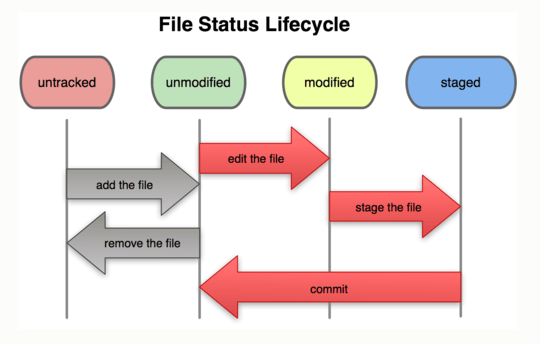
\includegraphics[width=0.70\textwidth]{figures/Git}}
 	\caption{File Status Lifecycle}
 	\label{File Status Lifecycle}
 \end{figure}
 
 
\noindent 
 \hspace*{0.5in} Git Init \par
\noindent 
Agar projek kita dapat diatur oleh git, maka kita perlu melakukan inisiasi git terlebih dahulu, caranya dengan mengetikkan perintah : \par
\vspace{\baselineskip}
\noindent 
 \hspace*{0.5in} git init \par
\noindent 
Perintah tersebut akan membuat folder .git dan didalamnya berisi file-file yang akan digunakan oleh Git untuk mengatur dan mengontrol project kita. \par
\vspace{\baselineskip}
\noindent 
 \hspace*{0.5in} Git Status \par
\noindent 
Untuk mengetahui status dari git, ketikkan perintah : \par
\vspace{\baselineskip}
\noindent 
 \hspace*{0.5in} git status \par
\noindent 
Anda akan mendapatkan keterangan seperti berikut: \par
\vspace{\baselineskip}
\noindent 
 \hspace*{0.5in} On branch master \par
\noindent 
 \hspace*{0.5in} Initial commit \par
\noindent 
 \hspace*{0.5in} nothing to commit (create/copy files and use "git add" to track) \par
\noindent 
Dari sana kita bisa mengetahui bahwa kita berada dalam branch master, dan kita telah melakukan initial commit, mengenai branch dan commit semuanya akan saya bahas nanti. \par
\noindent 
Sekarang mari kita buat file baru, misalkan buat file index.html lalu tambahkan kode berikut ke dalamnya \par
\begin{verbatim}
<!doctype html>
<html lang="en">
<head>
<meta charset="UTF-8"> 
<title>Belajar Git</title>
</head> 
<body> 
<p>Hello Git</p>
</body> 
</html> 
\end{verbatim}
\vspace{\baselineskip}
 \hspace*{0.5in} Git Add \par
\noindent 
Jika anda mengetikkan kembali perintah git status maka yang anda dapatkan kurang lebih seperti berikut : \par
\noindent 
On branch master~~~  \par
\noindent 
Initial commit \par
\noindent 
Untracked files: \par
\vspace{\baselineskip}
\noindent 
~  \hspace*{0.5in} (use "git add .." to include in what will be committed) \par
\noindent 
~~~  \hspace*{0.5in} index.html \par
\vspace{\baselineskip}
\noindent 
 \hspace*{0.5in} nothing added to commit but untracked files present (use "git add" to track) \par
\noindent 
Dari informasi diatas kita mendapatkan informasi bahwa Anda file baru yang belum terlacak. Kita perlu menambahkan file tersebut ke dalam git agar dapat dilacak perubahan-perubahan yang terjadi. Untuk itu anda dapat mengetikkan perintah: \par
\vspace{\baselineskip}
\noindent 
 \hspace*{0.5in} git add index.html \par
\noindent 
Dengan demikian anda telah menambahkan file index.html kedalam git agar bisa dimonitor/diawasi nantinya. Dan jika anda kembali mengetikkan git status yang akan anda dapatkan adalah: \par
\vspace{\baselineskip}
\noindent 
 \hspace*{0.5in} Changes to be committed: \par
\noindent 
 \hspace*{0.5in} ~~~ (use "git rm --cached .." to unstage) \par
\noindent 
 \hspace*{0.5in} ~~~~new~file:   index.html \par
 \vspace{\baselineskip}
\noindent 
 \hspace*{0.5in} Git Commit \par
\noindent 
Anda telah menambahkan file baru, namun anda belum melakukan commit. Oke, kembali ke contoh kasus dalam pembuka artikel ini, commit merupakan istilah untuk menandai terhadap perubahan yang telah anda lakukan, dalam contoh sebelumnya kita menandainya dengan tanggal dan keterangan singkat.  \par
\vspace{\baselineskip}
\noindent 
 \hspace*{0.5in} Nah untuk menandai setiap perubahan yang telah anda lakukan dan anda ingin agar git mengingatnya Anda harus melakukan commit terlebih dahulu. Untuk melakukan commit ketikkan perintah berikut: \par
 \vspace{\baselineskip}
\noindent 
 \hspace*{0.5in} git commit -m "Added index.html" \par
\noindent 
Dalam perintah diatas harus disertakan juga pesan commit, tanda -m digunakan untuk menambahkan pesan commit dan teks selanjutnya adalah pesan commit kita yakni  $ " $Added index.html $ " $. Jika semau anda lakukan dengan benar maka anda akan mendapatkan keterangan seperti berikut: \par
\vspace{\baselineskip}
\noindent 
 \hspace*{0.5in} [master (root-commit) 0181f7b] Added index.html \par
\noindent 
 \hspace*{0.5in}  1 file changed, 10 insertions(+) \par
\noindent 
 \hspace*{0.5in}  create mode 100644 index.html \par
\noindent 
 \hspace*{0.5in} Branch \par
 \vspace{\baselineskip}
\noindent 
Misalkan anda ingin menambahkan suatu fitur, namun anda tidak mau kode yang ada sekarang rusak karena fitur yang akan anda tambahkan masih belum stabil, Dalam Git anda dapat membuat branch terlebih dahulu. Branch ini bisa diartikan sebagai cabang dari branch master. segala perubahan yang anda lakukan pada branch yang anda buat tidak akan berpengaruh pada branch lainnya. \par
\noindent 
Sebagai contoh, kita buat branch dengan nama branch  $ " $fix-css $ " $ dengan mengetikkan perintah: \par
\vspace{\baselineskip}
\noindent 
 \hspace*{0.5in} git branch fix-css \par
 \vspace{\baselineskip}
\noindent 
Jika perintah dijalankan dengan benar maka ketika anda mengetikkan perintah git branch akan muncul branch-branch yang telah dibuat. \par
\vspace{\baselineskip}
\noindent 
 \hspace*{0.5in} ~~ fix-css \par
 \vspace{\baselineskip}
\noindent 
 \hspace*{0.5in} *~~ master \par
\noindent 
tanda Bintang menandakan bahwa anda sedang bekerja pada branch master, untuk berpindah ke branch yang baru saja dibuat (fix-css) ketikkan perintah berikut: \par
\vspace{\baselineskip}
\noindent 
 \hspace*{0.5in} git checkout fix-css \par
\noindent 
Jika peritah di atas benar, maka akan ada pemberitahuan seperti berikut: \par
\noindent 
 \hspace*{0.5in} Switched to branch 'fix-css' \par
 \vspace{\baselineskip}
\noindent 
\begin{itemize}
\item Github\end{itemize}
 \par
\noindent 
 \hspace*{0.5in} Github merupakan situs sharing code dan menggunakan git sebagai SCM-nya. Mungkin Anda pernah mendownload beberapa library/source code dari situs ini. Kini anda tahu mengapa kebanyakan source code dapat anda temui di github. \par
\vspace{12pt}
\noindent 
 \subsection{Apa itu GIT?} 
\noindent 
Git adalah version control, dengan menggunakan Git kita dapat menyimpan tiap perubahan yang kita lakukan pada file. Seperti menggunakan  $ " $undo $ " $ tetapi dapat digunakan pada seluruh file kita dan kita mempunyai log pada tiap perubahan yang kita simpan,  \par
\noindent 
Hal ini sangat berguna pada production environment, karena dengan adanya versioning, kita dapat dengan mudah melakukan rollback. Selain itu Git juga sangat membantu dalam proses pengembangan aplikasi. Salah satu platform Git yang terkenal adalah GitHub. Kita akan menggunakan GitHub untuk artiketl berikut. \par
\vspace{12pt}
\noindent 
\section{Repository}
\noindent 
Di Git Repository biasanya digunakan untuk mengorganisir sebuah projek. Projek dapat berisi files, folder, gambar, video dan lainnya yang dibutuhkan untuk sebuah project. Kami menyarankan untuk menambahkan file README yang bertujuan untuk memberi informasi terkait isi dari project tersebut. Kita dapat mengasumsikan Repository sebagai folder untuk menyimpan project kita. Satu berada di Local, dan yang satu berada di Remote disini kita menggunakan GitHub. \par
\vspace{\baselineskip}
\vspace{12pt}

{\fontsize{14pt}{14pt}\selectfont \textbf{Seperti Ini Perform Changes} \\} \par
\noindent 
 \hspace*{0.5in} Jerry mengkloning repositori dan memutuskan untuk menerapkan operasi string dasar. Jadi dia menciptakan file string.c. Setelah menambahkan isinya, string.c akan terlihat seperti berikut: \par
\vspace{12pt}
\noindent 
 \hspace*{0.5in}  $  \#  $include <stdio.h> \par
\noindent 
 \hspace*{0.5in} int my $  \_  $strlen (char * s) \hspace*{0.5in}  \par
\noindent 
 \hspace*{0.5in}  $  \{  $ \par
\noindent 
 \hspace*{0.5in}  $  $ $  $ $  $char * p = s; \par
\noindent 
 \hspace*{0.5in}  $  $ $  $ $  $sementara (* p) \par
\noindent 
 \hspace*{0.5in}  $  $ $  $ $  $ $  $ $  $ $  $++ p; \par
\noindent 
 \hspace*{0.5in}  $  $ $  $ $  $return (p - s); \par
\noindent 
 \hspace*{0.5in}  $  \}  $ \par
\noindent 
 \hspace*{0.5in} int main (void) \par
\noindent 
 \hspace*{0.5in}  $  \{  $ \par
\noindent 
 \hspace*{0.5in}  $  $ $  $ $  $int i; \par
\noindent 
 \hspace*{0.5in}  $  $ $  $ $  $char * s [] = \par
\noindent 
 \hspace*{0.5in}  $  $ $  $ $  $ $  \{  $ \par
\noindent 
 \hspace*{0.5in}  $  $ $  $ $  $ $  $ $  $ $  $"Git tutorial", \par
\noindent 
 \hspace*{0.5in}  $  $ $  $ $  $ $  $ $  $ $  $"Tutorial Point" \par
\noindent 
 \hspace*{0.5in}  $  $ $  $ $  $ $  \}  $; \par
\noindent 
 \hspace*{0.5in}  $  $ $  $ $  $untuk (i = 0; i <2; ++ i) $  $ $  $ $  $ $  $ $  $ $  $ \par
\noindent 
 $  $ $  $ $  $ \hspace*{0.5in} printf ("panjang string $  \%  $ s = $  \%  $ d  $  \setminus  $ n", s [i], my $  \_  $strlen (s [i])); \par
\noindent 
 \hspace*{0.5in}  $  $ $  $ $  $kembali 0; \par
\noindent 
 \hspace*{0.5in}  $  \}  $ \par
 \vspace{\baselineskip}
\noindent 
Dia menyusun dan menguji kodenya dan semuanya berjalan baik. Sekarang, dia bisa menambahkan perubahan ini ke repositori dengan aman. \par
\vspace{\baselineskip}
\noindent 
Git menambahkan operasi menambahkan file ke area stage. \par
\noindent 
 \hspace*{0.5in} [jerry @ CentOS project]  $  \$  $ git status -s \par
\noindent 
 \hspace*{0.5in} ?? tali \par
\noindent 
 \hspace*{0.5in} ?? string.c \par
\noindent 
 \hspace*{0.5in} [jerry @ CentOS project]  $  \$  $ git add string.c \par
 \vspace{\baselineskip}
\noindent 
Git menunjukkan tanda tanya sebelum nama file. Jelas, file-file ini bukan bagian dari Git, dan karena itulah Git tidak tahu apa yang harus dilakukan dengan file-file ini. Itu sebabnya, Git menunjukkan tanda tanya sebelum nama file. \par
\noindent 
Jerry telah menambahkan file ke area penyimpanan, perintah status git akan menampilkan file yang ada di area stage. \par
\vspace{\baselineskip}
\noindent 
 \hspace*{0.5in} [jerry @ CentOS project]  $  \$  $ git status -s \par
\noindent 
 \hspace*{0.5in} String.c \par
\noindent 
 \hspace*{0.5in} ?? tali \par
 \vspace{\baselineskip}
\noindent 
 \hspace*{0.5in} Untuk melakukan perubahan, dia menggunakan perintah komit git diikuti dengan opsi -m. Jika kita menghilangkan opsi -m. Git akan membuka text editor dimana kita bisa menulis multiline commit message. \par
 \vspace{\baselineskip}
\noindent 
 \hspace*{0.5in} [jerry @ CentOS project]  $  \$  $ git commit -m 'Implementasikan fungsi my $  \_  $strlen' \par
\noindent 
 \hspace*{0.5in} Perintah di atas akan menghasilkan hasil sebagai berikut: \par
\noindent 
 \hspace*{0.5in} [master cbe1249] Melaksanakan fungsi my $  \_  $strlen \par
\noindent 
 \hspace*{0.5in} 1 file berubah, 24 sisipan (+), 0 penghapusan (-) \par
\noindent 
 \hspace*{0.5in} buat mode 100644 string.c \par
 \vspace{\baselineskip}
\noindent 
Setelah berkomitmen untuk melihat rincian log, dia menjalankan perintah git log. Ini akan menampilkan informasi dari semua commit dengan commit komit mereka, commit author, commit date dan SHA-1 hash of commit. \par
\vspace{\baselineskip}
\noindent 
 \hspace*{0.5in} [jerry @ CentOS project]  $  \$  $ git log \par
 \vspace{\baselineskip}
\noindent 
Perintah di atas akan menghasilkan hasil sebagai berikut: \par
\noindent 
 \hspace*{0.5in} melakukan cbe1249b140dad24b2c35b15cc7e26a6f02d2277 \par
\noindent 
 \hspace*{0.5in} Penulis: Jerry Mouse <jerry@tutorialspoint.com> \par
\noindent 
 \hspace*{0.5in} Tanggal: Rabu Sep 11 08:05:26 2013 +0530 \par
\noindent 
 \hspace*{0.5in} Diimplementasikan fungsi my $  \_  $strlen \par
 \vspace{\baselineskip}
\noindent 
 \hspace*{0.5in}  \hspace*{0.5in} komit 19ae20683fc460db7d127cf201a1429523b0e319 \par
\noindent 
 \hspace*{0.5in}  \hspace*{0.5in} Penulis: Tom Cat <tom@tutorialspoint.com> \par
\noindent 
 \hspace*{0.5in}  \hspace*{0.5in} Tanggal: Rabu Sep 11 07:32:56 2013 +0530 \par
 \vspace{\baselineskip}
\noindent 
Komit awal \par
\noindent 
 \hspace*{0.5in} Jerry memeriksa versi terbaru dari repositori dan mulai mengerjakan sebuah proyek. Dia membuat file array.c di dalam direktori trunk. \par
 \vspace{\baselineskip}
 \vspace{\baselineskip}
\noindent 
 \hspace*{0.5in} [jerry @ CentOS  $  \sim  $]  $  \$  $ cd project $  \_  $repo / trunk / \par
\noindent 
 \hspace*{0.5in} [jerry @ CentOS trunk]  $  \$  $ cat array.c \par
\noindent 
 \hspace*{0.5in} Perintah di atas akan menghasilkan hasil berikut. \par
\noindent 
 \hspace*{0.5in}  $  \#  $include <stdio.h> \par
\noindent 
 \hspace*{0.5in}  $  \#  $define MAX 16 \par
\noindent 
 \hspace*{0.5in} int main (void)  $  \{  $ \par
\noindent 
 \hspace*{0.5in}  $  $ $  $ $  $int i, n, arr [MAX]; \par
\noindent 
 \hspace*{0.5in}  $  $ $  $ $  $printf ("Masukkan jumlah elemen:"); \par
\noindent 
 \hspace*{0.5in}  $  $ $  $ $  $scanf (" $  \%  $ d",  $  \&  $ n); \par
\noindent 
 \hspace*{0.5in}  $  $ $  $ $  $printf ("Enter the elements  $  \setminus  $ n"); \par
\noindent 
 \hspace*{0.5in}  $  $ $  $ $  $untuk (i = 0; i <n; ++ i) scanf (" $  \%  $ d",  $  \&  $ arr [i]); \par
\noindent 
 \hspace*{0.5in}  $  $ $  $ $  $printf ("Array memiliki elemen berikut  $  \setminus  $ n"); \par
\noindent 
 \hspace*{0.5in}  $  $ $  $ $  $untuk (i = 0; i <n; ++ i) printf (" $  \vert  $ $  \%  $ d  $  \vert  $", arr [i]); \par
\noindent 
 \hspace*{0.5in}  $  $ $  $ $  $printf (" $  \setminus  $ n"); \par
\noindent 
 \hspace*{0.5in}  $  $ $  $ $  $kembali 0; \par
\noindent 
 \hspace*{0.5in}  $  \}  $ \par
 \vspace{\baselineskip}
\noindent 
Dia ingin menguji kodenya sebelum melakukan. \par
\noindent 
 \hspace*{0.5in} [jerry @ CentOS trunk]  $  \$  $ buat array \par
\noindent 
 \hspace*{0.5in} cc array.c -o array \par
\noindent 
 \hspace*{0.5in} [jerry @ CentOS trunk]  $  \$  $ ./array \par
\noindent 
 \hspace*{0.5in} Masukkan jumlah elemen: 5 \par
\noindent 
 \hspace*{0.5in} Masukkan elemen \par
 \vspace{\baselineskip}
\noindent 
 \hspace*{0.5in}  \hspace*{0.5in} 1 \par
\noindent 
 \hspace*{0.5in}  \hspace*{0.5in} 2 \par
\noindent 
 \hspace*{0.5in}  \hspace*{0.5in} 3 \par
\noindent 
 \hspace*{0.5in}  \hspace*{0.5in} 4 \par
\noindent 
 \hspace*{0.5in}  \hspace*{0.5in} 5 \par
 \vspace{\baselineskip}
\noindent 
 \hspace*{0.5in} Array memiliki elemen berikut \par
\noindent 
 \hspace*{0.5in}  \hspace*{0.5in}  $  \vert  $ 1  $  \vert  $  $  \vert  $ 2  $  \vert  $  $  \vert  $ 3  $  \vert  $  $  \vert  $ 4  $  \vert  $  $  \vert  $ 5  $  \vert  $ \par
\vspace{12pt}
\vspace{\baselineskip}
\noindent 
Dia menyusun dan menguji kodenya dan semuanya berjalan seperti yang diharapkan, sekarang saatnya melakukan perubahan. \par
\vspace{\baselineskip}
\noindent 
 \hspace*{0.5in} [jerry @ CentOS trunk] status  $  \$  $ svn \par
\noindent 
 \hspace*{0.5in} ? array.c \par
\noindent 
 \hspace*{0.5in} ? array \par
 \vspace{\baselineskip}
\noindent 
Subversion menunjukkan '?' di depan nama file karena tidak tahu apa yang harus dilakukan dengan file-file ini. \par
\noindent 
Sebelum komit, Jerry perlu menambahkan file ini ke daftar perubahan yang tertunda. \par
\vspace{\baselineskip}
\vspace{\baselineskip}
\noindent 
 \hspace*{0.5in} [jerry @ CentOS trunk]  $  \$  $ svn tambahkan array.c \par
 \vspace{\baselineskip}
\noindent 
 \hspace*{0.5in} Sebuah array.c \par
 \vspace{\baselineskip}
\noindent 
Mari kita periksa dengan operasi 'status'. Subversion menunjukkan A sebelum array.c, artinya, file tersebut berhasil ditambahkan ke daftar perubahan yang tertunda. \par
\vspace{\baselineskip}
\noindent 
 \hspace*{0.5in} [jerry @ CentOS trunk] status  $  \$  $ svn \par
\noindent 
 \hspace*{0.5in} ? array \par
 \vspace{\baselineskip}
\noindent 
Sebuah array.c \par
\vspace{\baselineskip}
\noindent 
Untuk menyimpan file array.c ke repositori, gunakan perintah komit dengan opsi -m diikuti oleh pesan komit. Jika Anda menghilangkan opsi -m, Subversion akan menampilkan editor teks tempat Anda bisa mengetikkan pesan multi-baris. \par
\vspace{\baselineskip}
\noindent 
 \hspace*{0.5in} \vspace{12pt}
\noindent 
 \hspace*{0.5in} [jerry @ CentOS trunk]  $  \$  $ svn commit -m "Initial commit" \par
\noindent 
 \hspace*{0.5in} Menambahkan trunk / array.c \par
\noindent 
 \hspace*{0.5in} Mengirimkan data file \par
\noindent 
 \hspace*{0.5in} Komitmen revisi 2. \par
\noindent 
 \hspace*{0.5in} Sekarang file array.c berhasil ditambahkan ke repositori, dan nomor revisi bertambah satu. \par



\chapter{Review Changes}

\sloppy
\begin{center}{\fontsize{16pt}{16pt}\selectfont \textbf{MATERI GIT} \\}\end{center} \par
\noindent 
\begin{center}{\fontsize{14pt}{14pt}\selectfont \textbf{Git Riview}\textbf{ Changes} \\}\end{center} \par
\noindent 
{\fontsize{14pt}{14pt}\selectfont \textbf{Dasar Git} \\} \par
\noindent 
 \hspace*{0.5in} Jadi, sebenarnya apa yang dimaksud dengan Git? Ini adalah bagian penting untuk dipahami, karena jika anda memahami apa itu Git dan cara kerja, maka dapat dipastikan anda dapat menggunakan Git secara efektif dengan mudah. Selama menerapkan Git, cobalah untuk menggantikan VCS lain yang mungkin sudah anda kenal sebelumnya, misalnya Subversion dan Perforce. Git sangat berbeda dengan sistem-sistem ini dalam hal simpan atau informasi yang digunakan, meski antar muka sangat mirip. Dengan memahami perbedaan ini diharapkan dapat membantu anda menghindari penggunaan saat menggunakan Git. \par
\noindent 
Snapshot, Bukan Perbedaan \par
\noindent 
 \hspace*{0.5in} Salah satu perbedaan yang mencolok antar Git dengan VCS lainnya (Subversion dan kawan-kawan) adalah dalam cara Git para datanya. Konsep konseptual,. Sistem seperti ini (CVS, Subversion, Bazaar, dan yang lainnya) informasi yang tersimpannya sebagai sekumpulan berkas dan perubahan yang terjadi pada berkas-berkas tersebut, \par
\noindent 
Git dianggap datanya sebagai sebuah kumpulan snapshot dari sebuah miniatur sistem. Setiap kali anda melakukan komit, atau melakukan perubahan pada proyek Git anda, pada butir Git anda secara otomatis. Agar efisien, jika berkas tidak mengalami perubahan, Git tidak akan menyimpan file tersebut pada hanya pada file yang sama yang sebelumnya telah disimpan. \par
\noindent 
Git Punya Integritas \par
\noindent 
Segala sesuatu pada Git akan melalui proses checksum terlebih dahulu sebelum disimpan yang kemudian direferensikan oleh hasil checksum tersebut. Hal ini berarti tidak mungkin melakukan perubahan terhadap berkas manapun tanpa diketahui oleh Git.  \par
\noindent 
Fungsionalitas ini dimiliki oleh Git pada level terendahnya dan ini merupakan bagian tak terpisahkan dari filosofi Git. Anda tidak akan kehilangan informasi atau file yang tidak dimiliki oleh Git. \par
\noindent 
 \hspace*{0.5in} Mekanisme checksum yang digunakan oleh Git adalah SHA-1 hash. Ini merupakan sebuah susunan string yang terdiri dari 40 karakter heksadesimal (0 sampai 9 dan a sampai f) dan dihitung berdasarkan bentuk dari suatu berkas atau struktur pada pada Git. sebuah hash SHA-1 seperti berikut: \par
\noindent 
Anda akan melihat seperti ini pada berbagai tempat di Git. Faktanya, Git tidak memiliki nama file pada basisdatanya, pela nilai hash dari isi berkas. \par
\noindent 
Secara Umum Git Hanya Selesai Data \par
\noindent 
Bila anda melakukan operasi pada Git, hanya dari penambahan data pada basisdata Git. Sangat sulit membuat sistem melakukan sesuatu yang tidak bisa diurungkan atau membuatnya menghapus data dengan cara apa pun.  \par
\noindent 
Seperti pada berbagai VCS, anda bisa kehilangan atau mengacaukan perubahan yang belum di-commit; namun jika anda melakukan komit pada Git, akan sangat sulit kehilanngannya, apalagi jika anda secara teratur melakukan push basisdata anda pada repositori lain. Hal ini membuat Git menyenangkan karena kita dapat berexperimen tanpa kehawatiran untuk mengacaukan proyek. Untuk lebih jelas dan dalam lagi tentang bagaimana Git menyimpan datanya dan bagaimana anda bisa mengembalikan yang hilang \par
\noindent 
Direktori Git adalah dimana Git menyimpan metadata dan database objek untuk projek anda. Ini adalah bahagian penting dari Git, dan inilah yang disalin saat anda melakukan kloning sebuah repositori dari komputer lain. \par
\noindent 
Direktori kerja adalah sebuah checkout tunggal dari satu versi dari projek. File-berkas ini kemudian ditarik keluar dari basisdata yang terkompresi dalam direktori Git dan disimpan pada disk untuk anda pakai atau modifikasi. \par
\noindent 
 \hspace*{0.5in} Alur kerja dasar Git adalah seperti ini: \par
\noindent 
 \hspace*{0.5in} Anda mengubah berkas dalam direktori kerja anda. \par
\noindent 
 \hspace*{0.5in} Anda membawa ke tahap, menambahkan snapshotnya ke area stage. \par
\noindent 
 \hspace*{0.5in} Anda melakukan komit  \par
\noindent 
Jika sebuah versi tertentu dari sebuah berkas telah ada di direktori git, ia dianggap 'berkomitmen'. Jika berkas diubah (sudah diubah) maka sudah ditambahkan ke area stage, maka itu adalah 'staged'. Dan jika berkas telah diubah sejak terakhir dilakukan check out belum ditambahkan ke area stage maka itu adalah 'modified'. \par
\noindent 
Pada, anda akan lebih banyak membahas mengenai keadaan-keadaan ini dan bagaimana anda dapat memanfaatkan keadaan-keadaan yang bersangkutan dengan bagian 'bertahap'. \par
\noindent 
Git adalah $  $\textit{version control system} $  $yang digunakan para developer untuk mengembangkan software secara bersama-bersama. Fungsi utama git yaitu mengatur versi dari source code program anda dengan mengasih tanda baris dan code mana yang ditambah atau diganti.  Git ini sebenernya memudahkan programmer untuk mengetahui perubahan source codenya daripada harus membuat file baru seperti $  $\textit{Program.java, ProgramRevisi.java,}\textit{ }\textit{ProgramRevisi2.java, ProgramFix.java}. Selain itu, dengan git kita tak perlu khawatir code yang kita kerjakan bentrok, karena setiap developer bias membuat branch sebagai $  $\textit{workspace}nya.Fitur yang tak kalah keren lagi, pada git kita bisa memberi komentar pada source code yang telah ditambah/diubah, hal ini mempermudah developer lain untuk tahu $  $ kendala apa yang dialami developer lain. \par
\noindent 
Untuk mengetahui bagaimana menggunakan git, berikut perintah-perintah dasar git: \par
\noindent 
\begin{itemize}
\item Git init : untuk membuat $  $\textit{repository} $  $pada file lokal yang nantinya ada folder .git \par
\noindent 
\item Git status : untuk mengetahui status dari $  $\textit{repository} $  $lokal \par
\noindent 
\item Git add : menambahkan file baru pada $  $\textit{repository} $  $yang dipilih \par
\noindent 
\item Git commit : untuk menyimpan perubahan yang dilakukan, tetapi tidak ada perubahan pada $  $\textit{remote repository.} \par
\noindent 
\item Git push : untuk mengirimkan perubahan file setelah di commit ke $  $\textit{remote repository.} \par
\noindent 
\item Git branch : melihat seluruh $  $\textit{branch $  $}yang ada pada repository \par
\noindent 
\item Git checkout : menukar $  $\textit{branch $  $}yang aktif dengan $  $\textit{branch}yang dipilih \par
\noindent 
\item GIt merge : untuk menggabungkan $  $\textit{branch $  $}yang aktif dan $  $\textit{branch $  $}yang dipilih \par
\noindent 
\item Git clone : membuat Salinan $  $\textit{repository $  $}lokal\end{itemize}
 \par
\noindent 
Contoh dari $  $\textit{software version control system} $  $adalah github, bitbucket, snowy evening, dan masih banyak lagi. Jika anda sebagai developer belum mengetahui fitur git ini, maka anda wajib mencoba dan memakainya. Karena banyak manfaat yang akan didapat dengan git ini. \par
\noindent 
Git itu bukanlah sebuah bahasa seperti halnya HTML,CSS atau Js bukan pula sebuah konsep atau aturan baku dalam pemrograman, melainkan sebuah software yang berfungsi untuk mengatur source code dari aplikasi yang sedang anda buat. \par
\vspace{12pt}
\noindent 
Fungsi utamanya adalah untuk mengatur versi dari source code anda, menambahkan tanda/checkpoint ketika terjadi perubahan pada kode Anda dan tentunya akan mempermudah Anda untuk tetap mengetahui apa saja yang berubah dari source code Anda. \par
\noindent 
Sebagai contoh, misalkan Anda sedang membangun sebuah website, dan anda akan menambahkan beberapa fitur dalam website anda. Agar tidak membingungkan nantinya anda membuat sebuah catatan terhadap apa yang telah anda lakukan seperti : \par
\noindent 
 \hspace*{0.5in} 01-04-2014 Memulai Project Website, File HTML  $  \&  $ CSS Dasar \par
\noindent 
 \hspace*{0.5in} 02-04-2014 Penambahan Menu Utama \par
\noindent 
 \hspace*{0.5in} 03-04-2014 Penambahan Layout Standar \par
\noindent 
 \hspace*{0.5in} 04-04-2014 Penambahan Fitur Pengubah Layout \par
\noindent 
Pada contoh diatas kita menggunakan tanggal sebagai tanda akan apa yang telah kita lakukan, dengan demikian kita bisa tahu kapan perubahan terjadi dan apa perubahan yang dilakukan.  \par
\noindent 
Dan dalam Git semua itu bisa dilakukan dengan mudah dan asyiknya jika Anda merusak kode sehingga membuat aplikasi error, maka anda dapat mengembalikan kode tersebut berdasarkan pada tanda/tanggal dimana kode masih normal, lebih mirip seperti restore point. \par
\noindent 
Git juga tidak hanya digunakan untuk perorangan, beberapa orang pun dapat bekerja secara bersamaan mengerjakan kode Anda dan Anda masih memiliki kontrol penuh terhadap kode Anda,  \par
\noindent 
Anda bisa menambahkan kode yang ditambahan oleh orang lain atau mengabaikannya sama sekali. oleh karena itu Git sering digunakan sebagai pengatur dalam projek kolaborasi dimana tidak hanya satu orang yang mengerjakan sebuah kode tapi beberapa orang sekaligus yang mengerjakan kode tersebut. \par
\noindent 
Misalkan anda ingin menambahkan suatu fitur, namun anda tidak mau kode yang ada sekarang rusak karena fitur yang akan anda tambahkan masih belum stabil,  \par
\noindent 
Dalam Git anda dapat membuat branch terlebih dahulu. Branch ini bisa diartikan sebagai cabang dari branch master. segala perubahan yang anda lakukan pada branch yang anda buat tidak akan berpengaruh pada branch lainnya. \par
\noindent 
Sebagai contoh, kita buat branch dengan nama branch  $ " $fix-css $ " $ dengan mengetikkan perintah: \par
\noindent 
 \hspace*{0.5in} git branch fix-css \par
\noindent 
Jika perintah dijalankan dengan benar maka ketika anda mengetikkan perintah git branch akan muncul branch-branch yang telah dibuat. \par
\noindent 
 \hspace*{0.5in} ~~ fix-css \par
\noindent 
 \hspace*{0.5in} *~~ master \par
\noindent 
tanda Bintang menandakan bahwa anda sedang bekerja pada branch master, untuk berpindah ke branch yang baru saja dibuat (fix-css) ketikkan perintah berikut: \par
\noindent 
 \hspace*{0.5in} git checkout fix-css \par
\noindent 
Jika peritah di atas benar, maka akan ada pemberitahuan seperti berikut: \par
\noindent 
 \hspace*{0.5in} Switched to branch 'fix-css' \par
\noindent 
Github  \par
\noindent 
Github merupakan situs sharing code dan menggunakan git sebagai SCM-nya. Mungkin Anda pernah mendownload beberapa library/source code dari situs ini. Kini anda tahu mengapa kebanyakan source code dapat anda temui di github. \par
\vspace{12pt}
\noindent 
{\fontsize{14pt}{14pt}\selectfont \textbf{Apa}\textbf{ itu GIT?} \\} \par
\noindent 
Git adalah version control, dengan menggunakan Git kita dapat menyimpan tiap perubahan yang kita lakukan pada file. Seperti menggunakan  $ " $undo $ " $ tetapi dapat digunakan pada seluruh file kita dan kita mempunyai log pada tiap perubahan yang kita simpan, Hal ini sangat berguna pada production environment, karena dengan adanya versioning, kita dapat dengan mudah melakukan rollback. Selain itu Git juga sangat membantu dalam proses pengembangan aplikasi. Salah satu platform Git yang terkenal adalah GitHub. Kita akan menggunakan GitHub untuk artiketl berikut. \par
\vspace{12pt}
\noindent 
{\fontsize{14pt}{14pt}\selectfont \textbf{Repository} \\} \par
\noindent 
Di Git Repository biasanya digunakan untuk mengorganisir sebuah projek. Projek dapat berisi files, folder, gambar, video dan lainnya yang dibutuhkan untuk sebuah project. Kami menyarankan untuk menambahkan file README yang bertujuan untuk memberi informasi terkait isi dari project tersebut. Kita dapat mengasumsikan Repository sebagai folder untuk menyimpan project kita. Satu berada di Local, dan yang satu berada di Remote disini kita menggunakan GitHub. \par
\vspace{12pt}
\vspace{12pt}
\vspace{12pt}
\noindent 
\begin{center}{\fontsize{14pt}{14pt}\selectfont \textbf{REVIEW CHANGES} \\}\end{center} \par
\noindent 
{\fontsize{14pt}{14pt}\selectfont \textbf{Seperti Ini Review}\textbf{ Changes} \\} \par
\noindent 
Setelah melihat rincian komit, Jerry menyadari bahwa panjang string tidak boleh negatif, karena itulah dia memutuskan untuk mengubah jenis fungsi my $  \_  $strlen yang kembali. \par
\noindent 
 \hspace*{0.5in} Jerry menggunakan perintah git log untuk melihat detail log. \par
\noindent 
  $  \$  $ git log \par
\noindent 
Perintah di atas akan menghasilkan hasil berikut. \par
\noindent 
 \hspace*{0.5in}  \hspace*{0.5in} melakukan cbe1249b140dad24b2c35b15cc7e26a6f02d2277 \par
\noindent 
 \hspace*{0.5in} Penulis: Jerry Mouse <jerry@tutorialspoint.com> \par
\noindent 
 \hspace*{0.5in} Tanggal: Rabu Sep 11 08:05:26 2013 +0530 \par
\noindent 
 \hspace*{0.5in} Diimplementasikan fungsi my $  \_  $strlen \par
\noindent 
 \hspace*{0.5in} Jerry menggunakan perintah git show untuk melihat rincian komit. Perintah git show mengambil SHA-1 commit ID sebagai parameter. \par
\noindent 
 \hspace*{0.5in}  $  \$  $ git show cbe1249b140dad24b2c35b15cc7e26a6f02d2277 \par
\noindent 
 \hspace*{0.5in} Perintah di atas akan menghasilkan hasil sebagai berikut: \par
\noindent 
 \hspace*{0.5in} melakukan cbe1249b140dad24b2c35b15cc7e26a6f02d2277 \par
\noindent 
 \hspace*{0.5in} Penulis: Jerry Mouse <jerry@tutorialspoint.com> \par
\noindent 
 \hspace*{0.5in} Tanggal: Rabu Sep 11 08:05:26 2013 +0530 \par
\noindent 
 \hspace*{0.5in} Diimplementasikan fungsi my $  \_  $strlen \par
\noindent 
 \hspace*{0.5in} diff - git a / string.c b / string.c \par
\noindent 
 \hspace*{0.5in} mode file baru 100644 \par
\noindent 
 \hspace*{0.5in} indeks 0000000..187afb9 \par
\noindent 
 \hspace*{0.5in} --- / dev / null \par
\noindent 
 \hspace*{0.5in} +++ b / string.c \par
\noindent 
 \hspace*{0.5in} @@ -0,0 +1,24 @@ \par
\noindent 
 \hspace*{0.5in} +  $  \#  $ include <stdio.h> \par
\noindent 
 \hspace*{0.5in} + \par
\noindent 
 \hspace*{0.5in} + int my $  \_  $strlen (char * s) \par
\noindent 
 \hspace*{0.5in} +  $  \{  $ \par
\noindent 
 \hspace*{0.5in}  $  $ $  $ $  $+ \par
\noindent 
 \hspace*{0.5in}  $  $ $  $ $  $char * p = s; \par
\noindent 
 \hspace*{0.5in}  $  $ $  $ $  $+ \par
\noindent 
 \hspace*{0.5in}  $  $ $  $ $  $+ \par
\noindent 
 \hspace*{0.5in}  $  $ $  $ $  $sementara (* p) \par
\noindent 
 \hspace*{0.5in}  $  $ $  $ $  $+ ++ p; \par
\noindent 
 \hspace*{0.5in}  $  $ $  $ $  $+ return (p -s); \par
\noindent 
 \hspace*{0.5in}  $  $ $  $ $  $+ \par
\noindent 
 \hspace*{0.5in}  $  \}  $ \par
\noindent 
 \hspace*{0.5in} + \par
\noindent 
Dia mengubah jenis fungsi kembali dari int menjadi size $  \_  $t. Setelah menguji kode tersebut, dia mengulas perubahannya dengan menjalankan perintah diff git. \par
\noindent 
 \hspace*{0.5in}  $  \$  $ git diff \par
\noindent 
Perintah di atas akan menghasilkan hasil sebagai berikut: \par
\noindent 
 \hspace*{0.5in} diff - git a / string.c b / string.c \par
\noindent 
 \hspace*{0.5in} indeks 187afb9..7da2992 100644 \par
\noindent 
 \hspace*{0.5in} --- a / string.c \par
\noindent 
 \hspace*{0.5in} +++ b / string.c \par
\noindent 
 \hspace*{0.5in} @@ -1,6 +1,6 @@ \par
\noindent 
 \hspace*{0.5in}  $  \#  $include <stdio.h> \par
\noindent 
 \hspace*{0.5in} -int my $  \_  $strlen (char * s) \par
\noindent 
 \hspace*{0.5in} + size $  \_  $t my $  \_  $strlen (char * s) \par
\noindent 
 \hspace*{0.5in}  $  \{  $ \par
\noindent 
 \hspace*{0.5in}  $  $ $  $ $  $char * p = s; \par
\noindent 
 \hspace*{0.5in}  $  $ $  $ $  $@@ -18,7 +18,7 @@ int main (void) \par
\noindent 
 \hspace*{0.5in}  $  \}  $; \par
\noindent 
 \hspace*{0.5in} untuk (i = 0; i <2; ++ i) \par
\noindent 
 \hspace*{0.5in}  $  \{  $ \par
\noindent 
 \hspace*{0.5in}  $  $ $  $ $  $- printf ("panjang string $  \%  $ s = $  \%  $ d  $  \setminus  $ n", s [i], my $  \_  $strlen (s [i])); \par
\noindent 
 \hspace*{0.5in}  $  $ $  $ $  $+ printf ("panjang string $  \%  $ s = $  \%  $ lu  $  \setminus  $ n", s [i], my $  \_  $strlen (s [i])); \par
\noindent 
 \hspace*{0.5in}  $  $ $  $ $  $kembali 0; \par
\noindent 
 \hspace*{0.5in}  $  \}  $ \par
\noindent 
Git diff menunjukkan tanda '+' sebelum baris, yang baru ditambahkan dan '-' untuk baris yang dihapus. \par
\noindent 
Melihat Sejarah Komit \par
\noindent 
 \hspace*{0.5in} Setelah Anda membuat beberapa commit, atau jika Anda telah mengkloning sebuah repositori dengan riwayat komit yang ada, Anda mungkin ingin melihat kembali untuk melihat apa yang telah terjadi. Alat yang paling dasar dan ampuh untuk melakukan ini adalah perintah git log. \par
\noindent 
Contoh-contoh ini menggunakan proyek sederhana yang disebut "simplegit". Untuk mendapatkan proyek, jalankan \par
\noindent 
git klon https://github.com/schacon/simplegit-progit \par
\noindent 
Saat Anda menjalankan git log dalam proyek ini, Anda harus mendapatkan keluaran yang terlihat seperti ini: \par
\noindent 
 \hspace*{0.5in}  $  \$  $ git log \par
\noindent 
 \hspace*{0.5in} melakukan ca82a6dff817ec66f44342007202690a93763949 \par
\noindent 
 \hspace*{0.5in} Penulis: Scott Chacon <schacon@gee-mail.com> \par
\noindent 
 \hspace*{0.5in} Tanggal: Sen 17 Mar 21:52:11 2008 -0700 \par
\noindent 
 \hspace*{0.5in}  $  $ $  $ $  $ $  $mengubah nomor versinya \par
\noindent 
 \hspace*{0.5in} komit 085bb3bcb608e1e8451d4b2432f8ecbe6306e7e7 \par
\noindent 
 \hspace*{0.5in} Penulis: Scott Chacon <schacon@gee-mail.com> \par
\noindent 
 \hspace*{0.5in} Tanggal: Sat 15 Mar 16:40:33 2008 -0700 \par
\noindent 
lepaskan tes yang tidak perlu \par
\noindent 
 \hspace*{0.5in} lakukan a11bef06a3f659402fe7563abf99ad00de2209e6 \par
\noindent 
 \hspace*{0.5in} Penulis: Scott Chacon <schacon@gee-mail.com> \par
\noindent 
 \hspace*{0.5in} Tanggal: Sat Mar 15 10:31:28 2008 -0700 \par
\noindent 
 $  $ $  $ $  $ $  $komit pertama \par
\noindent 
Secara default, tanpa argumen, git log mencantumkan komit yang dibuat di repositori tersebut dalam urutan kronologis terbalik - yaitu, komit terbaru muncul lebih dulu. Seperti yang dapat Anda lihat, perintah ini mencantumkan masing-masing komit dengan checksum SHA-1, nama penulis dan e-mail, tanggal penulisan, dan pesan komit. \par
\noindent 
Sejumlah besar dan berbagai pilihan untuk perintah git log tersedia untuk menunjukkan dengan tepat apa yang Anda cari. Di sini, kami akan menunjukkan beberapa yang paling populer. \par
\noindent 
Salah satu pilihan yang lebih bermanfaat adalah -p, yang menunjukkan perbedaan yang diperkenalkan pada masing-masing komit. Anda juga bisa menggunakan -2, yang membatasi output hanya pada dua entri terakhir: \par
\noindent 
 \hspace*{0.5in}  $  \$  $ git log -p -2 \par
\noindent 
 \hspace*{0.5in} melakukan ca82a6dff817ec66f44342007202690a93763949 \par
\noindent 
 \hspace*{0.5in} Penulis: Scott Chacon <schacon@gee-mail.com> \par
\noindent 
 \hspace*{0.5in} Tanggal: Sen 17 Mar 21:52:11 2008 -0700 \par
\noindent 
 \hspace*{0.5in}  $  $ $  $ $  $ $  $mengubah nomor versinya \par
\noindent 
 \hspace*{0.5in} diff - git a / Rakefile b / Rakefile \par
\noindent 
 \hspace*{0.5in} indeks a874b73..8f94139 100644 \par
\noindent 
 \hspace*{0.5in} --- a / Rakefile \par
\noindent 
 \hspace*{0.5in} +++ b / Rakefile \par
\noindent 
 \hspace*{0.5in} @@ -5,7 +5,7 @@ memerlukan 'rake / gempackagetask' \par
\noindent 
 \hspace*{0.5in}  $  $spec = Gem :: Specification.new do  $  \vert  $ s  $  \vert  $ \par
\noindent 
 \hspace*{0.5in}  $  $ $  $ $  $ $  $ $  $s.platform = Gem :: Platform :: RUBY \par
\noindent 
 \hspace*{0.5in}  $  $ $  $ $  $ $  $ $  $s.name = "simplegit" \par
\noindent 
 \hspace*{0.5in} - s.version = "0.1.0" \par
\noindent 
 \hspace*{0.5in} + s.version = "0.1.1" \par
\noindent 
 \hspace*{0.5in}  $  $ $  $ $  $ $  $ $  $s.author = "Scott Chacon" \par
\noindent 
 \hspace*{0.5in}  $  $ $  $ $  $ $  $ $  $s.email = "schacon@gee-mail.com" \par
\noindent 
 \hspace*{0.5in}  $  $ $  $ $  $ $  $ $  $s.summary = "Sebuah permata sederhana untuk menggunakan Git dalam kode Ruby." \par
\noindent 
 \hspace*{0.5in} komit 085bb3bcb608e1e8451d4b2432f8ecbe6306e7e7 \par
\noindent 
 \hspace*{0.5in} Penulis: Scott Chacon <schacon@gee-mail.com> \par
\noindent 
 \hspace*{0.5in} Tanggal: Sat 15 Mar 16:40:33 2008 -0700 \par
\noindent 
 \hspace*{0.5in}  $  $ $  $ $  $ $  $lepaskan tes yang tidak perlu \par
\noindent 
 \hspace*{0.5in}  \hspace*{0.5in} diff - git a / lib / simplegit.rb b / lib / simplegit.rb \par
\noindent 
 \hspace*{0.5in}  \hspace*{0.5in} indeks a0a60ae..47c6340 100644 \par
\noindent 
 \hspace*{0.5in}  \hspace*{0.5in} --- a / lib / simplegit.rb \par
\noindent 
 \hspace*{0.5in}  \hspace*{0.5in} +++ b / lib / simplegit.rb \par
\noindent 
 \hspace*{0.5in}  \hspace*{0.5in} @@ -18,8 +18,3 @@ kelas SimpleGit \par
\noindent 
 \hspace*{0.5in}  \hspace*{0.5in}  $  $ $  $ $  $ $  $ $  $akhir \par
\noindent 
 \hspace*{0.5in}  $  $akhir \par
\noindent 
 \hspace*{0.5in} - \par
\noindent 
 \hspace*{0.5in} -if  $  \$  $ 0 ==  $  \_  $ $  \_  $FILE $  \_  $ $  \_  $ \par
\noindent 
 \hspace*{0.5in} - git = SimpleGit.new \par
\noindent 
 \hspace*{0.5in} - menempatkan git.show \par
\noindent 
 \hspace*{0.5in} -akhir \par
\noindent 
 \hspace*{0.5in}  $  \setminus  $ Tidak ada baris baru di akhir file \par
\noindent 
 \hspace*{0.5in} Pilihan ini menampilkan informasi yang sama namun dengan diff langsung mengikuti setiap entri. Ini sangat membantu untuk tinjauan kode atau untuk menelusuri dengan cepat apa yang terjadi selama serangkaian komit yang telah ditambahkan oleh kolaborator. Anda juga bisa menggunakan serangkaian opsi merangkum dengan log git. Misalnya, jika Anda ingin melihat beberapa statistik singkat untuk setiap komit, Anda dapat menggunakan opsi --stat: \par
\noindent 
 \hspace*{0.5in}  $  \$  $ git log --stat \par
\noindent 
 \hspace*{0.5in} melakukan ca82a6dff817ec66f44342007202690a93763949 \par
\noindent 
 \hspace*{0.5in} Penulis: Scott Chacon <schacon@gee-mail.com> \par
\noindent 
 \hspace*{0.5in} Tanggal: Sen 17 Mar 21:52:11 2008 -0700 \par
\noindent 
 \hspace*{0.5in}  $  $ $  $ $  $ $  $mengubah nomor versinya \par
\noindent 
 \hspace*{0.5in}  $  $Rakefile  $  \vert  $ 2 + - \par
\noindent 
 \hspace*{0.5in}  $  $1 file berubah, 1 insertion (+), 1 deletion (-) \par
\noindent 
 \hspace*{0.5in} komit 085bb3bcb608e1e8451d4b2432f8ecbe6306e7e7 \par
\noindent 
 \hspace*{0.5in} Penulis: Scott Chacon <schacon@gee-mail.com> \par
\noindent 
 \hspace*{0.5in} Tanggal: Sat 15 Mar 16:40:33 2008 -0700 \par
\noindent 
 \hspace*{0.5in}  $  $ $  $ $  $ $  $lepaskan tes yang tidak perlu \par
\noindent 
 \hspace*{0.5in}  $  $lib / simplegit.rb  $  \vert  $ 5 ----- \par
\noindent 
 \hspace*{0.5in}  $  $1 file berubah, 5 deletions (-) \par
\noindent 
 \hspace*{0.5in} lakukan a11bef06a3f659402fe7563abf99ad00de2209e6 \par
\noindent 
 \hspace*{0.5in} Penulis: Scott Chacon <schacon@gee-mail.com> \par
\noindent 
 \hspace*{0.5in} Tanggal: Sat Mar 15 10:31:28 2008 -0700 \par
\noindent 
 \hspace*{0.5in}  $  $ $  $ $  $ $  $komit pertama \par
\noindent 
 $  $ \hspace*{0.5in}  \hspace*{0.5in} README  $  \vert  $ 6 ++++++ \par
\noindent 
 \hspace*{0.5in}  $  $ \hspace*{0.5in} Rakefile  $  \vert  $ 23 +++++++++++++++++++++++ \par
\noindent 
 $  $ \hspace*{0.5in}  \hspace*{0.5in} lib / simplegit.rb  $  \vert  $ 25 +++++++++++++++++++++++++ \par
\noindent 
 \hspace*{0.5in}  \hspace*{0.5in}  $  $3 file berubah, 54 sisipan (+) \par



\chapter{Commit Cahnges}

\begin{figure}[ht]
	\centerline{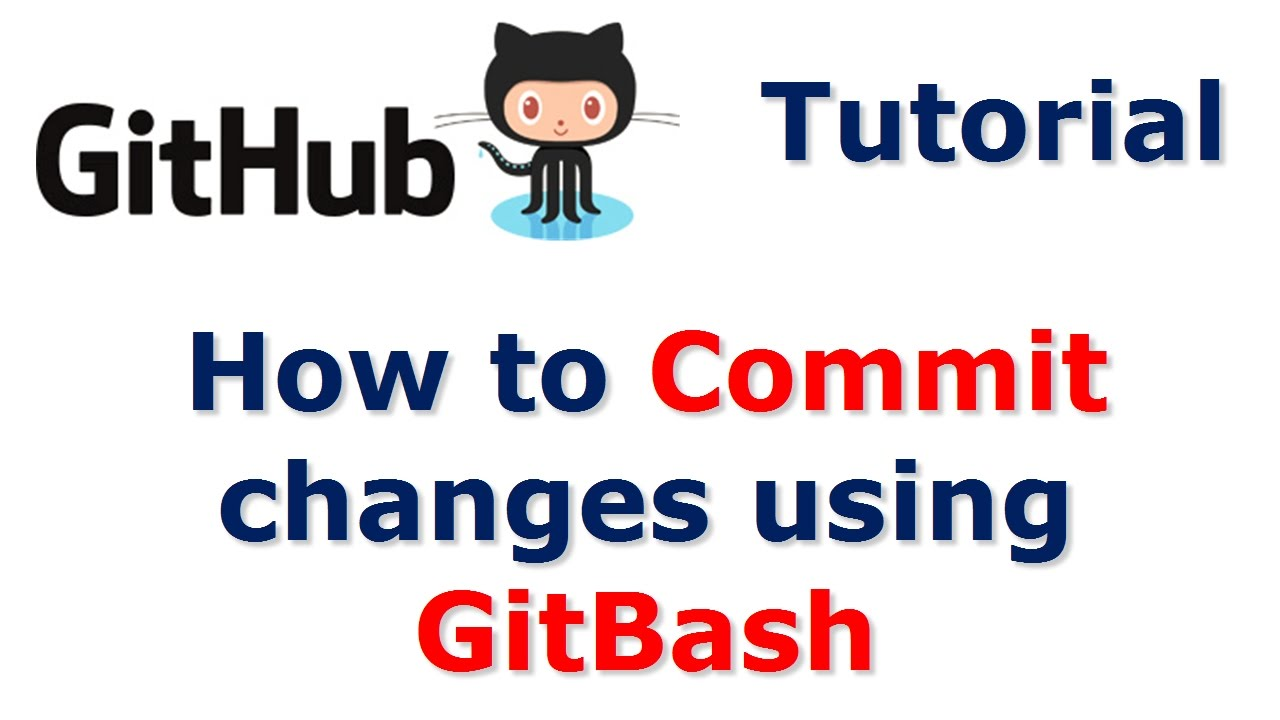
\includegraphics[width=0.80\textwidth]{Figures/dapgit1.jpg}}
	\caption{Commit Changes}
	\label{Commit Changes}
\end{figure}


\section {Pengertian }
\subsection {Commit Changes}
Melakukan perubahan perubahan tentunya anda sudah memiliki repositori Git yang bonafide dan sebuah salinan kerja dari semua berkas untuk proyek tersebut. Anda harus membuat beberapa perubahan dan commit perubahan tersebut ke dalam repositori setiap saat proyek mencapai sebuah keadaan yang ingin Anda rekam.Ingat bahwa setiap berkas di dalam direktori kerja Anda dapat berada di 2 keadaan: terpantau atau tak-terpantau. Berkas terpantau adalah berkas yang sebelumnya berada di snapshot terakhir; mereka dapat berada dalam kondisi belum terubah, terubah, ataupun staged (berada di area stage). Berkas tak-terpantau adalah kebalikannya - merupakan berkas-berkas di dalam direktori kerja yang tidak berada di dalam snapshot terakhir dan juga tidak berada di area staging. Ketika Anda pertama kali menduplikasi sebuah repositori, semua berkas Anda akan terpantau dan belum terubah karena Anda baru saja melakukan checkout dan belum mengubah apapun.Cek Status Anda Alat utama yang Anda gunakan untuk menentukan berkas-berkas mana yang berada dalam keadaan tertentu adalah melalui perintah git status. Jika Anda menggunakan alat ini langsung setelah sebuah clone, Anda akan melihat serupa seperti di bawah ini: \par
\noindent 
 $  \$  $ git status \par
\noindent 
 $  \#  $ On branch master \par
\noindent 
nothing to commit, working directory clean \par
\noindent 
Ini berarti Anda memiliki direktori kerja yang bersih-dengan kata lain, tidak ada berkas terpantau yang terubah. Git juga tidak melihat berkas-berkas yang tak terpantau, karena pasti akan dilaporkan oleh alat ini. Juga, perintah ini memberitahu Anda tentang cabang tempat Anda berada. Pada saat ini, cabang akan selalu berada di master, karena sudah menjadi default-nya; Anda tidak perlu khawatir tentang cabang dulu. Bab berikutnya akan membahas tentang percabangan dan referensi secara lebih detil. \par
\noindent 


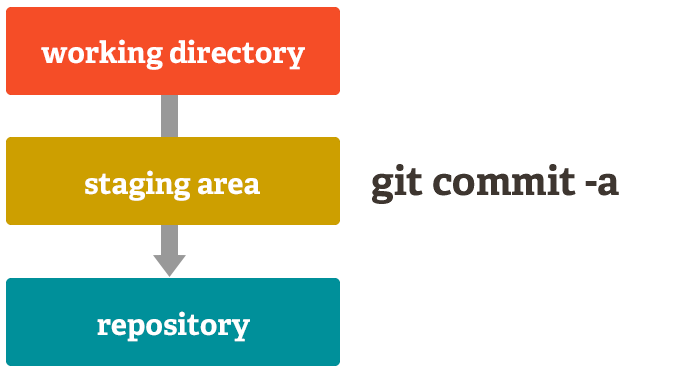
\includegraphics[width=10cm,height=7cm]{Figures/dapigit2.jpg}
\begin{equation}python regular expression\end{equation}


Mari kita umpamakan Anda menambah sebuah berkas baru ke dalam proyek Anda, misalnya sesederhana berkas README. Jika file tersebut belum ada sebelumnya, dan Anda melakukan git status, Anda akan melihatnya sebagai berkas tak-terpantau seperti berikut ini: \par
\vspace{12pt}
\noindent 
\begin{verbatim}
 $  \$  $ vim README \par
\noindent 
 $  \$  $ git status \par
\noindent 
 $  \#  $ On branch master \par
\noindent 
 $  \#  $ Untracked files: \par
\noindent 
 $  \#  $~~ (use "git add <file>..." 
 to include in what will be committed) \par
\noindent 
 $  \#  $ \par
\noindent 
 $  \#  $~~ README \par
\noindent 
nothing added to commit but
 untracked files present (use "git add" to track) 

\end{verbatim}
Anda akan melihat bahwa berkas baru Anda README belum terpantau, karena berada di bawah judul "Untracked files" di keluaran status Anda. Untracked pada dasarnya berarti bahwa Git melihat sebuah berkas yang sebelumnya tidak Anda miliki di snapshot (commit) sebelumnya; Git tidak akan mulai memasukkannya ke dalam snapshot commit hingga Anda secara eksplisit memerintahkan Git. Git berlaku seperti ini agar Anda tidak secara tak-sengaja mulai menyertakan berkas biner hasil kompilasi atau berkas lain yang tidak Anda inginkan untuk disertakan. Anda hanya ingin mulai menyertakan README, mari kita mulai memantau berkas tersebut. \par
\vspace{12pt}
\noindent 
 \section{Berikut adalah langkah-langkah untuk menjalankan perintah}
 
  \begin{enumerate}


\item Untuk mulai memantau berkas baru, Anda menggunakan perintah git add. Untuk mulai memantau berkas README tadi, Anda menjalankannya seperti berikut: \par
\vspace{12pt}
\noindent 
\begin{verbatim}
 $  \$  $ git add README
 
 \end{verbatim}
  \par
\vspace{12pt}
\noindent 

\item Jika Anda menjalankan perintah status lagi, Anda akan melihat bahwa berkas README Anda sekarang sudah terpantau dan sudah masuk ke dalam area stage: \par
\vspace{12pt}
\noindent 

\begin{verbatim}
 $  \$  $ git status \par
\noindent 
 $  \#  $ On branch master \par
\noindent 
 $  \#  $ Changes to be committed: \par
\noindent 
 $  \#  $~~ (use "git reset HEAD <file>..." to unstage) \par
\noindent 
 $  \#  $ \par
\noindent 
 $  \#  $~~~new~file:   README \par
\noindent 
 $  \#  $ \par
\noindent 

 \end{verbatim}

\item Anda dapat mengatakan bahwa berkas tersebut berada di dalam area stage karena tertulis di bawah judul "Changes to be committed". Jika Anda melakukan commit pada saat ini, versi berkas pada saat Anda menjalankan git add inilah yang akan dimasukkan ke dalam sejarah snapshot. Anda mungkin ingat bahwa ketika Anda menjalankan git init sebelumnya, Anda melanjutkannya dengan git add (nama berkas) - yang akan mulai dipantau di direktori Anda. Perintah git add ini mengambil alamat dari berkas ataupun direktori; jika sebuah direktori, perintah tersebut akan menambahkan seluruh berkas yang berada di dalam direktori secara rekursif. \par
\vspace{12pt}
\noindent 

\item Mari kita ubah sebuah berkas yang sudah terpantau. Jika Anda mengubah berkas yang sebelumnya terpantau bernama benchmarks.rb dan kemudian menjalankan perintah status lagi, Anda akan mendapatkan keluaran kurang lebih seperti ini: \par
\vspace{12pt}
\noindent 
\begin{verbatim}
 $  \$  $ git status \par
\noindent 
 $  \#  $ On branch master \par
\noindent 
 $  \#  $ Changes to be committed: \par
\noindent 
 $  \#  $~~ (use "git 
 reset HEAD <file>..." 
 to unstage) \par
\noindent 
 $  \#  $ \par
\noindent 
 $  \#  $~~~new~file:   README \par
\noindent 
 $  \#  $ \par
\noindent 
 $  \#  $ Changes not staged for commit: \par
\noindent 
 $  \#  $~~ (use "git add <file>..."
  to update what will be committed) \par
\noindent 
 $  \#  $ \par
\noindent 
 $  \#  $~~~modified:~  benchmarks.rb \par
\noindent 
 $  \#  $ \par
\vspace{12pt}
\vspace{12pt}
\noindent 
 \end{verbatim}

\item Berkas benchmarks.rb terlihat di bawah bagian yang bernama "Changes not staged for commit" - yang berarti bahwa sebuah berkas terpantau telah berubah di dalam direktori kerja namun belum masuk ke area stage. Untuk memasukkannya ke area stage, Anda menjalankan perintah git add (perintah ini adalah perintah multiguna - Anda menggunakannya untuk mulai memantau berkas baru, untuk memasukkannya ke area stage, dan untuk melakukan hal lain seperti menandai berkas terkonflik menjadi terpecahkan). Mari kita sekarang jalankan git add untuk memasukkan berkas benchmarks.rb ke dalam area stage, dan jalankan git status lagi: \par
\vspace{12pt}
\noindent 

\begin{verbatim}


 $  \$  $ git add benchmarks.rb \par
\noindent 
 $  \$  $ git status \par
\noindent 
 $  \#  $ On branch master \par
\noindent 
 $  \#  $ Changes to be committed: \par
\noindent 
 $  \#  $~~ (use "git reset HEAD
  <file>..." to unstage) \par
\noindent 
 $  \#  $ \par
\noindent 
 $  \#  $~~~new~file:   README \par
\noindent 
 $  \#  $~~~modified:~  benchmarks.rb \par
\noindent 
 $  \#  $ \par
\vspace{12pt}
\vspace{12pt}
\vspace{12pt}
\noindent 

\end{verbatim}

\item Kedua file sekarang berada di area stage dan akan masuk ke dalam commit Anda berikutnya. Pada saat ini, semisal Anda teringat satu perubahan yang Anda ingin buat di benchmarks.rb sebelum Anda lakukan commit. Anda buka berkas tersebut kembali dan melakukan perubahan tersebut, dan Anda siap untuk melakukan commit. Namun, mari kita coba jalankan git status kembali: \par
\vspace{12pt}
\vspace{12pt}
\vspace{12pt}
\noindent 

\begin{verbatim}



 $  \$  $ vim benchmarks.rb  \par
\noindent 
 $  \$  $ git status \par
\noindent 
 $  \#  $ On branch master \par
\noindent 
 $  \#  $ Changes to be committed: \par
\noindent 
 $  \#  $~~ (use "git reset HEAD <file>..."
  to unstage) \par
\noindent 
 $  \#  $ \par
\noindent 
 $  \#  $~~~new~file:   README \par
\noindent 
 $  \#  $~~~modified:~  benchmarks.rb \par
\noindent 
 $  \#  $ \par
\noindent 
 $  \#  $ Changes not staged for commit: \par
\noindent 
 $  \#  $~~ (use "git add <file>..."
  to update what will be committed) \par
\noindent 
 $  \#  $ \par
\noindent 
 $  \#  $~~~modified:~  benchmarks.rb \par
\noindent 
 $  \#  $ \par
\vspace{12pt}
\noindent 
\end{verbatim}


\item Apa? Sekarang benchmarks.rb terdaftar di dua tempat: area stage dan area terubah. Bagaimana hal ini bisa terjadi? Ternyata Git memasukkan berkas ke area stage tepat seperti ketika Anda menjalankan perintah git add. Jika Anda commit sekarang, versi benchmarks.rb pada saat Anda terakhir lakukan perintah git add-lah yang akan masuk ke dalam commit, bukan versi berkas yang saat ini terlihat di direktori kerja Anda ketika Anda menjalankan git commit. Jika Anda mengubah sebuah berkas setelah Anda menjalankan git add, Anda harus menjalankan git add kembali untuk memasukkan versi berkas terakhir ke dalam area stage: \par
\vspace{12pt}
\vspace{12pt}
\noindent 

\begin{verbatim}



 $  \$  $ git add benchmarks.rb \par
\noindent 
 $  \$  $ git status \par
\noindent 
 $  \#  $ On branch master \par
\noindent 
 $  \#  $ Changes to be committed: \par
\noindent 
 $  \#  $~~ (use "git reset HEAD <file>..."
  to unstage) \par
\noindent 
 $  \#  $ \par
\noindent 
 $  \#  $~~~new~file:   README \par
\noindent 
 $  \#  $~~~modified:~  benchmarks.rb \par
\noindent 
 $  \#  $ \par
 
 \end{verbatim}
 
\vspace{12pt}
\vspace{12pt}
\noindent 


\end{enumerate}

\section{Tambahkan secara otomatis}

Terkadang, Anda memiliki sekumpulan berkas yang Anda tidak ingin Git tambahkan secara otomatis atau bahkan terlihat sebagai tak-terpantau. Biasanya berkas hasil keluaran seperti berkas log atau berkas yang dihasilkan oleh sistem build Anda. Dalam kasus ini, Anda dapat membuat sebuah berkas bernama .gitignore yang berisi pola dari berkas terabaikan. Berikut adalah sebuah contoh isi dari berkas .gitignore: \par
\noindent 
 $  \$  $ cat .gitignore \par
\noindent 
*.[oa] \par
\noindent 
* $  \sim  $ \par
\noindent 
Baris pertama memberitahu Git untuk mengabaikan semua file yang berakhiran .o atau .a - berkas object dan arsip yang mungkin dihasilkan dari kompilasi kode Anda. Baris kedua memberitahu Git untuk mengabaikan semua file yang berakhiran dengan sebuah tilde ( $  \sim  $), yang biasanya digunakan oleh banyak aplikasi olah-kata seperti Emacs untuk menandai berkas sementara. Anda juga dapat memasukkan direktori log, tmp ataupun pid; dokumentasi otomatis; dan lainnya. Menata berkas .gitignore sebelum Anda mulai bekerja secara umum merupakan ide yang baik sehingga Anda tidak secara tak-sengaja melakukan commit terhadap berkas yang sangat tidak Anda inginkan berada di dalam repositori Git. \par
\noindent 
Aturan untuk pola yang dapat Anda gunakan di dalam berkas .gitignore adalah sebagai berikut: \par
\noindent 
\begin{itemize}
\item Baris kosong atau baris dimulai dengan  $  \#  $ akan diabaikan. \par
\noindent 
\item Pola glob standar dapat digunakan. \par
\noindent 
\item Anda dapat mengakhir pola dengan sebuah slash (/) untuk menandai sebuah direktori. \par
\noindent 
\item Anda dapat menegasikan sebuah pola dengan memulainya menggunakan karakter tanda seru (!).\end{itemize}
 \par
\noindent 
Pola Glob adalah seperti regular expression yang disederhanakan yang biasanya digunakan di shell. Sebuah asterisk (*) berarti 0 atau lebih karakter; [abc] terpasangkan dengan karakter apapun yang ditulis dalam kurung siku (dalam hal ini a, b, atau c); sebuah tanda tanya (?) terpasangkan dengan sebuah karakter; dan kurung siku yang melingkupi karakter yang terpisahkan dengan sebuah tanda hubung([0-9]) terpasangkan dengan karakter apapun yang berada diantaranya (dalam hal ini 0 hingga 9). \par
\noindent 
Berikut adalah contoh lain dari isi berkas .gitignore: \par
\noindent 
 $  \#  $ sebuah komentar – akan diabaikan \par
\noindent 
 $  \#  $ abaikan berkas .a \par
\noindent 
*.a \par
\noindent 
 $  \#  $ tapi pantau lib.a, walaupun Anda abaikan berkas .a di atas \par
\noindent 
!lib.a \par
\noindent 
 $  \#  $ hanya abaikan berkas TODO yang berada di rooto, bukan di subdir/TODO \par
\noindent 
/TODO \par
\noindent 
 $  \#  $ abaikan semua berkas di dalam direktori build/ \par
\noindent 
build/ \par
\noindent 
 $  \#  $ abaikan doc/notes.txt, tapi bukan doc/server/arch.txt \par
\noindent 
doc/*.txt \par
\noindent 
Jika perintah git status terlalu kabur untuk Anda - Anda ingin mengetahui secara pasti apa yang telah berubah, bukan hanya berkas mana yang berubah - Anda dapat menggunakan perintah git diff. Kita akan bahas git diff secara lebih detil nanti; namun Anda mungkin menggunakannya paling sering untuk menjawab 2 pertanyaan berikut: Apa yang Anda ubah tapi belum dimasukkan ke area stage? Dan apa yang telah Anda ubah yang akan segera Anda commit? Walaupun git status menjawab pertanyaan tersebut secara umum, git diff menunjukkan kepada Anda dengan tepat baris yang ditambahkan dan dibuang - dalam bentuk patch-nya. \par
\noindent 
Mari kita anggap Anda mengubah dan memasukkan berkas README ke area stage lagi dan kemudian mengubah berkas benchmarks.rb tanpa memasukkannya ke area stage. Jika Anda jalankan perintah status Anda, Anda akan sekali lagi melihat keluaran seperti berikut: \par
\vspace{12pt}
\noindent 
git status \par
\noindent 
 $  \#  $ On branch master \par
\noindent 
 $  \#  $ Changes to be committed: \par
\noindent 
 $  \#  $~~ (use "git reset HEAD <file>..." to unstage) \par
\noindent 
 $  \#  $ \par
\noindent 
 $  \#  $~~~new~file:   README \par
\noindent 
 $  \#  $ \par
\noindent 
 $  \#  $ Changes not staged for commit: \par
\noindent 
 $  \#  $~~ (use "git add <file>..." to update what will be committed) \par
\noindent 
 $  \#  $ \par
\noindent 
 $  \#  $~~~modified:~  benchmarks.rb \par
\noindent 
 $  \#  $ \par
\noindent 
Untuk melihat apa yang Anda telah ubah namun belum masuk ke area stage, ketikkan git diff tanpa argumen lainnya. \par
\vspace{12pt}
\noindent 
git diff \par
\noindent 
diff --git a/benchmarks.rb b/benchmarks.rb \par
\noindent 
index 3cb747f..da65585 100644 \par
\noindent 
--- a/benchmarks.rb \par
\noindent 
+++ b/benchmarks.rb \par
\noindent 
@@ -36,6 +36,10 @@ def main \par
\noindent 
~~~~~~~~~~ @commit.parents[0].parents[0].parents[0] \par
\noindent 
~~~~~~~~ end \par
\vspace{12pt}
\noindent 
+~~~~~~~ run $  \_  $code(x, 'commits 1') do \par
\noindent 
+~~~~~~~~~ git.commits.size \par
\noindent 
+~~~~~~~ end \par
\noindent 
+ \par
\noindent 
~~~~~~~~ run $  \_  $code(x, 'commits 2') do \par
\noindent 
~~~~~~~~~~ log = git.commits('master', 15) \par
\noindent 
~~~~~~~~~~ log.size \par
\noindent 
Perintah di atas membandingkan apa yang ada di direktori kerja Anda dengan apa yang ada di area stage. Hasilnya memberitahu Anda bahwa perubahan yang Anda ubah namun belum masuk ke area stage. \par
\noindent 
Jika Anda ingin melihat apa yang telah Anda masukkan ke area stage yang nantinya akan masuk ke commit Anda berikutnya, Anda dapat menggunakan git diff --cached. (Di Git versi 1.6.1 atau yang lebih tinggi, Anda dapat juga menggunakan git diff --staged, yang mungkin lebih mudah untuk diingat). Perintah ini membandingkan area stage Anda dengan commit Anda terakhir: \par
\vspace{12pt}
\vspace{12pt}
\noindent 
 $  \$  $ git diff --cached \par
\noindent 
diff --git a/README b/README \par
\noindent 
new file mode 100644 \par
\noindent 
index 0000000..03902a1 \par
\noindent 
--- /dev/null \par
\noindent 
+++ b/README2 \par
\noindent 
@@ -0,0 +1,5 @@ \par
\noindent 
+grit \par
\noindent 
+ by Tom Preston-Werner, Chris Wanstrath \par
\noindent 
+ http://github.com/mojombo/grit \par
\noindent 
+ \par
\noindent 
+Grit is a Ruby library for extracting information from a Git repository \par
\noindent 
Satu hal penting yang harus dicatat adalah bahwa git diff saja tidak memperlihatkan semua perubahan yang telah Anda lakukan sejak terakhir Anda commit - hanya perubahan yang belum masuk ke area stage saja. Mungkin agak sedikit membingungkan, karena jika Anda telah memasukkan semua perubahan ke area stage, git diff akan memberikan keluaran kosong. \par
\noindent 
Sebagai contoh lain, jika Anda memasukkan berkas benchmarks.rb ke area stage dan kemudian meng-editnya, Anda dapat menggunakan git diff untuk melihat perubahan di berkas tersebut yang telah masuk ke area stage dan perubahan yang masih di luar area stage: \par
\noindent 
 $  \$  $ git add benchmarks.rb \par
\noindent 
 $  \$  $ echo ' $  \#  $ test line' >> benchmarks.rb \par
\noindent 
 $  \$  $ git status \par
\noindent 
 $  \#  $ On branch master \par
\noindent 
 $  \#  $ \par
\noindent 
 $  \#  $ Changes to be committed: \par
\noindent 
 $  \#  $ \par
\noindent 
 $  \#  $~~~modified:~  benchmarks.rb \par
\noindent 
 $  \#  $ \par
\noindent 
 $  \#  $ Changes not staged for commit: \par
\noindent 
 $  \#  $ \par
\noindent 
 $  \#  $~~~modified:~  benchmarks.rb \par
\noindent 
 $  \#  $ \par
\noindent 
Sekarang Anda dapat menggunakan git diff untuk melihat apa saja yang masih belum dimasukkan ke area stage: \par
\vspace{12pt}
\noindent 
 $  \$  $ git diff  \par
\noindent 
diff --git a/benchmarks.rb b/benchmarks.rb \par
\noindent 
index e445e28..86b2f7c 100644 \par
\noindent 
--- a/benchmarks.rb \par
\noindent 
+++ b/benchmarks.rb \par
\noindent 
@@ -127,3 +127,4 @@ end \par
\noindent 
 main() \par
\vspace{12pt}
\noindent 
  $  \#  $ $  \#  $pp Grit::GitRuby.cache $  \_  $client.stats  \par
\noindent 
+ $  \#  $ test line \par
\vspace{12pt}
\noindent 
dan git diff --cached untuk melihat apa yang telah Anda masukkan ke area stage sejauh ini: \par
\vspace{12pt}
\noindent 
 $  \$  $ git diff --cached \par
\noindent 
diff --git a/benchmarks.rb b/benchmarks.rb \par
\noindent 
index 3cb747f..e445e28 100644 \par
\noindent 
--- a/benchmarks.rb \par
\noindent 
+++ b/benchmarks.rb \par
\noindent 
@@ -36,6 +36,10 @@ def main \par
\noindent 
~~~~~~~~~ @commit.parents[0].parents[0].parents[0] \par
\noindent 
~~~~~~~ end \par
\vspace{12pt}
\noindent 
+~~~~~~~ run $  \_  $code(x, 'commits 1') do \par
\noindent 
+~~~~~~~~~ git.commits.size \par
\noindent 
+~~~~~~~ end \par
\noindent 
+~~~~~~~~~~~~~  \par
\noindent 
~~~~~~~ run $  \_  $code(x, 'commits 2') do \par
\noindent 
~~~~~~~~~ log = git.commits('master', 15) \par
\noindent 
~~~~~~~~~ log.size \par
\vspace{12pt}
\vspace{12pt}
\noindent 
Sekarang setelah area stage Anda tertata sebagaimana yang Anda inginkan, Anda dapat melakukan commit terhadap perubahan Anda. Ingat bahwa apapun yang masih di luar area stage - berkas apapun yang Anda telah buat atau ubah yang belum Anda jalankan git add terhadapnya sejak terakhir Anda edit - tidak akan masuk ke dalam commit ini. Perubahan tersebut akan tetap sebagai berkas terubah di cakram Anda. Dalam hal ini, saat terakhir Anda jalankan git status, Anda telah melihat bahwa semuanya telah masuk ke stage, sehingga Anda siap untuk melakukan commit dari perubahan Anda. Cara termudah untuk melakukan commit adalah dengan mengetikkan git commit: \par
\vspace{12pt}
\noindent 
 $  \$  $ git commit \par
\noindent 
Dengan melakukan ini, aplikasi olahkata pilihan Anda akan terjalankan (Ini ditata oleh variabel lingkungan  $  \$  $EDITOR di shell Anda - biasanya vim atau emacs, walaupun Anda dapat mengkonfigurasinya dengan apapun yang Anda inginkan menggunakan perintah git config -- global core.editor yang telah Anda lihat di Bab 1). \par
\noindent 
Aplikasi olahkata akan menampilakn teks berikut (contoh berikut adalah dari layar Vim): \par
\vspace{12pt}
\vspace{12pt}
\noindent 
 $  \#  $ Please enter the commit message for your changes. Lines starting \par
\noindent 
 $  \#  $ with ' $  \#  $' will be ignored, and an empty message aborts the commit. \par
\noindent 
 $  \#  $ On branch master \par
\noindent 
 $  \#  $ Changes to be committed: \par
\noindent 
 $  \#  $~~ (use "git reset HEAD <file>..." to unstage) \par
\noindent 
 $  \#  $ \par
\noindent 
 $  \#  $~~~~~~~new~file:   README \par
\noindent 
 $  \#  $~~~~~~~modified:~  benchmarks.rb  \par
\noindent 
 $  \sim  $ \par
\noindent 
 $  \sim  $ \par
\noindent 
 $  \sim  $ \par
\noindent 
".git/COMMIT $  \_  $EDITMSG" 10L, 283C \par
\vspace{12pt}
\vspace{12pt}
\noindent 
Anda dapat melihat bahwa pesan commit standar berisi keluaran terakhir dari perintah git status yang terkomentari dan sebuah baris kosong di bagian atas. Anda dapat membuang komentar-komentar ini dan mengetikkan pesan commit Anda, atau Anda dapat membiarkannya untuk membantu Anda mengingat apa yang akan Anda commit. (Untuk pengingat yang lebih eksplisit dari apa yang Anda ubah, Anda dapat menggunakan opsi -v di perintah git commit. Melakukan hal ini akan membuat diff dari perubahan Anda di dalam olahkata sehingga Anda dapat melihat secara tepat apa yang telah Anda lakukan). Ketika Anda keluar dari olahkata, Git akan membuat commit Anda dengan pesan yang Anda buat (dengan bagian terkomentari dibuang). \par
\noindent 
Cara lainnya, Anda dapat mengetikkan pesan commit Anda sebaris denegan perintah commit dengan mencantumkannya setelah tanda -m seperti berikut: \par
\vspace{12pt}
\vspace{12pt}
\noindent 
 $  \$  $ git commit -m "Story 182: Fix benchmarks for speed" \par
\noindent 
[master]: created 463dc4f: "Fix benchmarks for speed" \par
\noindent 
 2 files changed, 3 insertions(+), 0 deletions(-) \par
\noindent 
 create mode 100644 README \par
\vspace{12pt}
\vspace{12pt}
\noindent 
Sekarang Anda telah membuat commit pertama Anda $  \sim  $ Anda dapat lihat bahwa commit tersebut telah memberi Anda beberapa keluaran tentang dirinya sendiri: cabang apa yang Anda jadikan target commit (master), ceksum SHA-1 apa yang commit tersebut miliki (463dc4f), berapa banyak berkas yang diubah, dan statistik tentang jumlah baris yang ditambah dan dibuang dalam commit tersebut. \par
\noindent 
Ingat bahwa commit merekam snapshot yang Anda telah tata di area stage. Apapun yang tidak Anda masukkan ke area stage akan tetap berada di tempatnya, tetap dalam keadaan terubah; Anda dapat melakukan commit lagi untuk memasukkannya ke dalam sejarah Anda. Setiap saat Anda melakukan sebuah commit, Anda merekamkan sebuah snapshot dari proyek Anda yang bisa Anda kembalikan atau Anda bandingkan nantinya. \par
\noindent 
Walaupun dapat menjadi sangat berguna untuk menata commit tepat sebagaimana Anda inginkan, area stage terkadang sedikit lebih kompleks dibandingkan apa yang Anda butuhkan di dalam alurkerja Anda. Jika Anda ingin melewatkan area stage, Git menyediakan sebuah jalan pintas sederhana. Dengan memberikan opsi -a ke perintah git commit akan membuat Git secara otomatis menempatkan setiap berkas yang telah terpantau ke area stage sebelum melakukan commit, membuat Anda dapat melewatkan bagian git add: \par
\vspace{12pt}
\noindent 
 $  \$  $ git status \par
\noindent 
 $  \#  $ On branch master \par
\noindent 
 $  \#  $ \par
\noindent 
 $  \#  $ Changes not staged for commit: \par
\noindent 
 $  \#  $ \par
\noindent 
 $  \#  $~~~modified:~  benchmarks.rb \par
\noindent 
 $  \#  $ \par
\noindent 
 $  \$  $ git commit -a -m 'added new benchmarks' \par
\noindent 
[master 83e38c7] added new benchmarks \par
\noindent 
 1 files changed, 5 insertions(+), 0 deletions(-) \par
\vspace{12pt}
\noindent 
Perhatikan bagaimana Anda tidak perlu menjalankan git add terhadap berkas benchmarks.rb dalam hal ini sebelum Anda commit. \par
\noindent 
\textbf{M}\textbf{enghapus sebuah berkas dari Git} \par
\noindent 
Untuk menghapus sebuah berkas dari Git, Anda harus menghapusnya dari berkas terpantau (lebih tepatnya, mengpus dari area stage) dan kemudian commit. Perintah git rm melakukan hal tadi dan juga menghapus berkas tersebut dari direktori kerja Anda sehingga Anda tidak melihatnya sebagai berkas yang tak terpantau nantinya. \par
\noindent 
Jika Anda hanya menghapus berkas dari direktori kerja Anda, berkas tersebut akan muncul di bagian "Changes not staged for commit" (yaitu, di luar area stage) dari keluaran git status Anda: \par
\noindent 
 $  \$  $ rm grit.gemspec \par
\noindent 
 $  \$  $ git status \par
\noindent 
 $  \#  $ On branch master \par
\noindent 
 $  \#  $ \par
\noindent 
 $  \#  $ Changes not staged for commit: \par
\noindent 
 $  \#  $~~ (use "git add/rm <file>..." to update what will be committed) \par
\noindent 
 $  \#  $ \par
\noindent 
 $  \#  $~~~~~~~deleted:~~  grit.gemspec \par
\noindent 
 $  \#  $ \par
\vspace{12pt}
\vspace{12pt}
\noindent 
Kemudian, jika Anda jalankan git rm, Git akan memasukkan penghapusan berkas tersebut ke area stage: \par
\vspace{12pt}
\noindent 
 $  \$  $ git rm grit.gemspec \par
\noindent 
rm 'grit.gemspec' \par
\noindent 
 $  \$  $ git status \par
\noindent 
 $  \#  $ On branch master \par
\noindent 
 $  \#  $ \par
\noindent 
 $  \#  $ Changes to be committed: \par
\noindent 
 $  \#  $~~ (use "git reset HEAD <file>..." to unstage) \par
\noindent 
 $  \#  $ \par
\noindent 
 $  \#  $~~~~~~~deleted:~~  grit.gemspec \par
\noindent 
 $  \#  $ \par
\vspace{12pt}
\vspace{12pt}
\noindent 
Pada saat Anda commit nantinya, berkas tersebut akan hilang dan tidak lagi terpantau. Jika Anda mengubah berkas tersebut dan menambahkannya lagi ke index, Anda harus memaksa penghapusannya dengan menggunakan opsi -f. Ini adalah fitur keamanan (safety) untuk mencegah ketidaksengajaan penghapusan terhadap data yang belum terekam di dalam snapshot dan tak dapat dikembalikan oleh Git. \par
\noindent 
Hal berguna lain yang Anda dapat lakukan adalah untuk tetap menyimpan berkas di direktori kerja tetapi menghapusnya dari area kerja. Dengan kata lain, Anda mungkin ingin tetap menyimpan berkas tersebut di dalam cakram keras tetapi tidak ingin Git untuk memantaunya lagi. Hal ini khususnya berguna jika Anda lupa untuk menambahkan sesuaitu ke berkas .gitignore Anda dan secara tak-sengaja menambahkannya, seperti sebuah berkas log yang besar, atau sekumpulan berkas hasil kompilasi .a. Untuk melakukan ini, gunakan opsi --cached: \par
\vspace{12pt}
\noindent 
 $  \$  $ git rm --cached readme.txt \par
\noindent 
Anda dapat menambahkan nama berkas, direktori, dan pola glob ke perintah git rm. Ini berarti Anda dapat melakukan hal seperti \par
\vspace{12pt}
\noindent 
 $  \$  $ git rm log/ $  \setminus  $*.log \par
\noindent 
Perhatikan karakter backslash ( $  \setminus  $) di depan tanda *. Ini dibutuhkan agar Git juga meng-ekspansi nama berkas sebagai tambahan dari ekspansi nama berkas oleh shell Anda. Perintah ini mengapus semua berkas yang memiliki ekstensi .log di dalam direktori log/. Atau, Anda dapat melakukannya seperti ini: \par
\noindent 
 $  \$  $ git rm  $  \setminus  $* $  \sim  $ \par
\noindent 
Tidak seperti kebanyakan sistem VCS lainnya, Git tidak secara eksplisit memantau perpindahan berkas. Jika Anda mengubag nama berkas di Git, tidak ada metada yang tersimpan di Git yang menyatakan bahwa Anda mengubah nama berkas tersebut. Namun demikian, Git cukup cerdas untuk menemukannya berdasarkan fakta yang ada - kita akan membicarakan tentang mendeteksi perpindahan berkas sebentar lagi. \par
\noindent 
Untuk itu agak membingungkan bahwa Git memiliki perintah mv. Jika Anda hendak mengubah nama berkas di Git, Anda dapat menjalankan seperti berikut \par
\noindent 
 $  \$  $ git mv file $  \_  $from file $  \_  $to \par
\noindent 
dan itu berjalan baik. Bahkan, jika Anda menjalankannya seperti ini kemudian melihat ke status, Anda akan melihat bahwa Git menganggapnya sebagai perintah pengubahan nama berkas.  \par
\noindent 
 $  \$  $ git mv README.txt README \par
\noindent 
 $  \$  $ git status \par
\noindent 
 $  \#  $ On branch master \par
\noindent 
 $  \#  $ Your branch is ahead of 'origin/master' by 1 commit. \par
\noindent 
 $  \#  $ \par
\noindent 
 $  \#  $ Changes to be committed: \par
\noindent 
 $  \#  $~~ (use "git reset HEAD <file>..." to unstage) \par
\noindent 
 $  \#  $ \par
\noindent 
 $  \#  $~~~~~~~renamed:~~  README.txt -> README \par
\noindent 
 $  \#  $ \par
\noindent 
Namun sebetulnya hal ini serupa dengan menjalankan perintah-perintah berikut: \par
\noindent 
 $  \$  $ mv README.txt README \par
\noindent 
 $  \$  $ git rm README.txt \par
\noindent 
 $  \$  $ git add README \par
\noindent 
Git mengetahui secara implisit bahwa perubahan yang terjadi merupakan proses pengubahan nama, sehingga sebetulnya tidaklah terlalu bermasalah jika Anda mengubah nama sebuah berkas dengan cara ini atau dengan menggunakan perintah mv. Satu-satunya perbedaan utama adalah mv berjumlah satu perintah dan bukannya tiga - yang membuat fungsi ini lebih nyaman digunakan. Lebih penting lagi, Anda sebetulnya dapat menggunakan alat apapun yang Anda suka untuk mengubah nama berkas, tinggal tambahkan perintah add/rm di bagian akhir, sesaat sebelum Anda melakukan commit. \par
\vspace{12pt}
\vspace{12pt}
\vspace{12pt}
\vspace{12pt}


\chapter{Push Operation}

\sloppy
\begin{center}{\fontsize{16pt}{16pt}\selectfont Push Operation \\}\end{center} \par


\begin{figure}[ht]
	\centerline{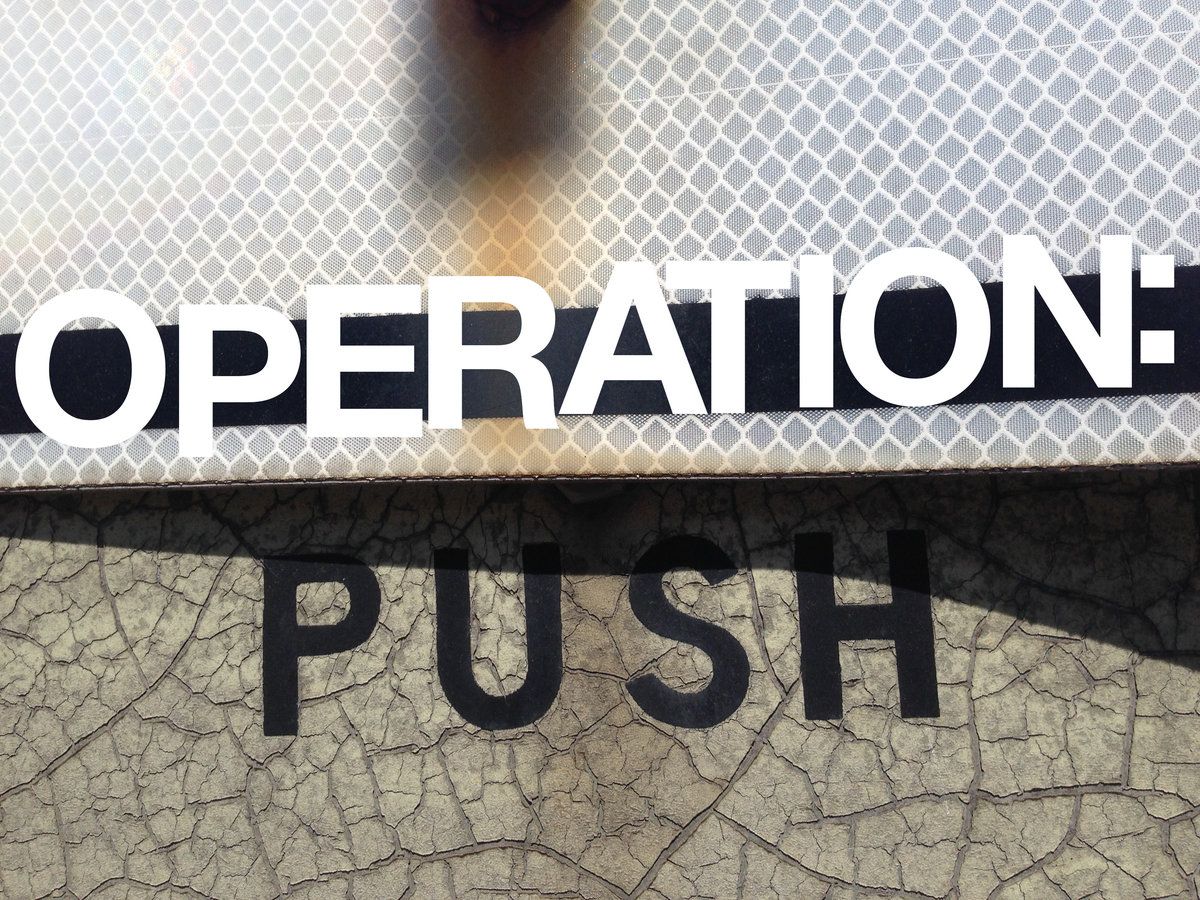
\includegraphics[width=0.60\textwidth]{Figures/dapgit3.jpg}}
	\caption{Push Operation}
	\label{Push Operation}
\end{figure}





\section {Pengertian }
\subsection {Push Operation}



Bekerja dalam satu proyek secara bersama-sama sudah menjadi hal yang lumrah sekarang ini. Termasuk juga proyek-proyek dalam dunia komputer yang sebagian besar menuliskan kode untuk menciptakan software, sistem informasi, aplikasi, atau apa pun namanya. Salah satu sistem yang banyak dipakai untuk membantu pengerjaan proyek bersama tersebut adalah Source Control Management (SCM) atau disebut juga dengan Version Control System (VCS). Ada banyak contoh produk-produk yang tergolong ke dalam jenis VCS, salah satunya adalah Git. Git adalah VCS yang dibangun oleh Linus Torvalds, dikenal juga sebagai pencipta sistem operasi linux, untuk membantu pengembangan kernel linux. Sebelum menggunakan git, pengembangan kernel linux menggunakan produk VCS bernama BitKeeper. Ketika BitKeeper telah menjadi software yang berbayar dan tidak menjadi produk opensource lagi, maka Linus menciptakan Git sebagai pengganti dalam pengembangan kernel linux. \par
Git adalah VCS yang banyak digunakan saat ini. Banyak pengerjaan proyek bersama menggunakan bantuan Git untuk mengelola artefak proyek. Github, salah satu layanan VCS berbasis Git dengan web-based interface, telah menjadi tempat dikembangkannya proyek-proyek open source diseluruh dunia. Tidak hanya untuk proyek opensource, Github juga dapat digunakan untuk mengerjakan proyek non-opensource. \par
\noindent 
Jadi kenapa Git begitu spesial? \par
\noindent 
Bersifat tersebar, sifat tersebar menyebabkan Git terhindar dari permasalahan kegagalan disatu titik. Jika terjadi kerusakan repo pada salah satu mesin maka dapat dipulihkan dengan menyalin repo yang sama dari mesin yang berbeda. Sifat tersebar juga memudahkan developer untuk menjalankan aplikasi dalam rangka \textit{debugging $  $}karena seluruh artifak proyek ada pada mesin developer tersebut. \par
\noindent 
Opensource, Git dikembangkan dengan tujuan untuk membantu pengembangan kernel linux yang bersifat opensource. Konsep Git dapat dipastikan memenuhi aspek-aspek pendukung pengerjaan proyek-proyek opensource. Satu hal yang pasti bahwa git bebas digunakan tanpa pusing memikirkan lisensi. \par
\noindent 
Snapshots, Bukan Perbedaan, Berbeda $  $dengan VCS lain yang umumnya melakukan pencatatan artefak proyek dengan konsep daftar perubahan file (\textit{list of file-based changes}), $  $ $  $Git melakukan pencatatan terhadap artefak proyek dengan konsep seperti pengambilan foto \textit{(snapshot). $  $}Konsep daftar perubahan file akan menyalin seluruh file pada versi sebelumnya untuk dimasukan pada versi sekarang walaupun tidak terjadi perubahan pada file tersebut. Konsep \textit{snapshot $  $}akan mengambil gambaran artefak proyek secara keseluruhan pada versi pertama. Versi selanjutnya dibuat dengan cara menyimpan perbedaan antara versi sekarang dengan versi selanjutnya ditambah dengan penghubung (\textit{pointer, link}) ke snapshot pada versi sekarang. Jadi konsep snapshot tidak mencatat file yang tidak berubah secara berulang-ulang dan juga tidak kehilangan informasi mengenai versi sebelumnya. \par
\noindent 
Hampir Seluruh Operasi Tidak Melibatkan Jaringan, Konsep terdistribusi pada Git menyebabkan git dapat beroperasi tanpa melibatkan mesin lain secara umum. Hal ini berbeda dengan Centralized VCS(CVCS)yang hampir seluruh operasinya memerlukan koneksi jaringan. Sebagai contoh ketika kita berada di pesawat terbang , kereta api, ataupun area lain yang tidak memiliki jaringan ke server proyek yang sedang dikerjakan, maka kita tidak bisa bekerja secara optimal jika menggunakan CVCS. \par
\noindent 
Git Memiliki Integritas, Segala sesuatu pada Git akan diberi tanda khusus \textit{(checksum) $  $}sebelum disimpan ke dalam database. Hal ini menghindari terjadi\textit{ file corruption} tanpa diketahui oleh Git. Git menggunakan algoritma SHA-1 untuk melakukan \textit{checksum} tersebut. \par
\noindent 
Konsep Tiga Status, $  $Git memiliki 3 status utama dalam melakukan pencatatan terhadap artefak proyek. Konsep 3 status ini adalah kunci utama dalam memahami penggunaan Git secara baik dan benar. Jadi pastikan developer paham dengan konsep 3 status pada Git sebelum menggunakannya. Jika dirasa perlu maka dapat dikumpulkan informasi yang lebih banyak tentang konsep ini untuk mempermudah penggunaan Git kedepannya. File pada Git memiliki salah satu dari 3 status berikut: \textit{commited, modified,} dan \textit{staged. Commited $  $}artinya perubahan terhadap file telah disimpan ke dalam database Git. \textit{Modified} artinya telah terjadi perubahan pada file dan perubahan sama sekali belum disimpan oleh Git. \textit{Staged} artinya perubahan pada file telah tersimpan ke dalam penyimpanan sementara dan siap untuk disimpan ke dalam database. Konsep 3 status menyebabkan proyek pada Git terbagi atas 3 bagian utama yaitu: database Git (\textit{Git directory or Git database or Git Repository}), area kerja (\textit{working directory}), dan area perantara (\textit{staging area})  \par
\noindent 
Database git adalah tempat dimana Git menyimpan seluruh informasi tambahan dan perubahan-perubahan untuk setiap versi artefak proyek. Ini adalah bagian yang sangat penting dari Git dan bagian ini adalah bagian yang akan disalin dalam proses \textit{cloning repository $  $}dari satu mesin ke mesin yang lain. Area kerja adalah folder induk yang mengandung seluruh artefak proyek (file-file) yang sedang dikerjakan. Area perantara adalah tempat menyimpan informasi perubahan terhadap artefak proyek yang siap untuk disimpan ke dalam database Git. Bentuk nyatanya adalah sebuah file yang terletak di dalam direktori Git. Area perantara terkadang disebut juga sebagai index.\vspace{\baselineskip}
\section{Alur kerja Git yang paling umum adalah sebagai berikut} \par


\begin{enumerate}


\item Developer melakukan perubahan terhadap file yang berada pada area kerja \par
\item Developer menyimpan perubahan ke dalam area perantara untuk proses pengambil \textit{snapshot} \par
\item Developer menyimpan perubahan secara permanen ke dalam database Git \par
\vspace{12pt}
\vspace{12pt}
\noindent 
\end {enumerate}


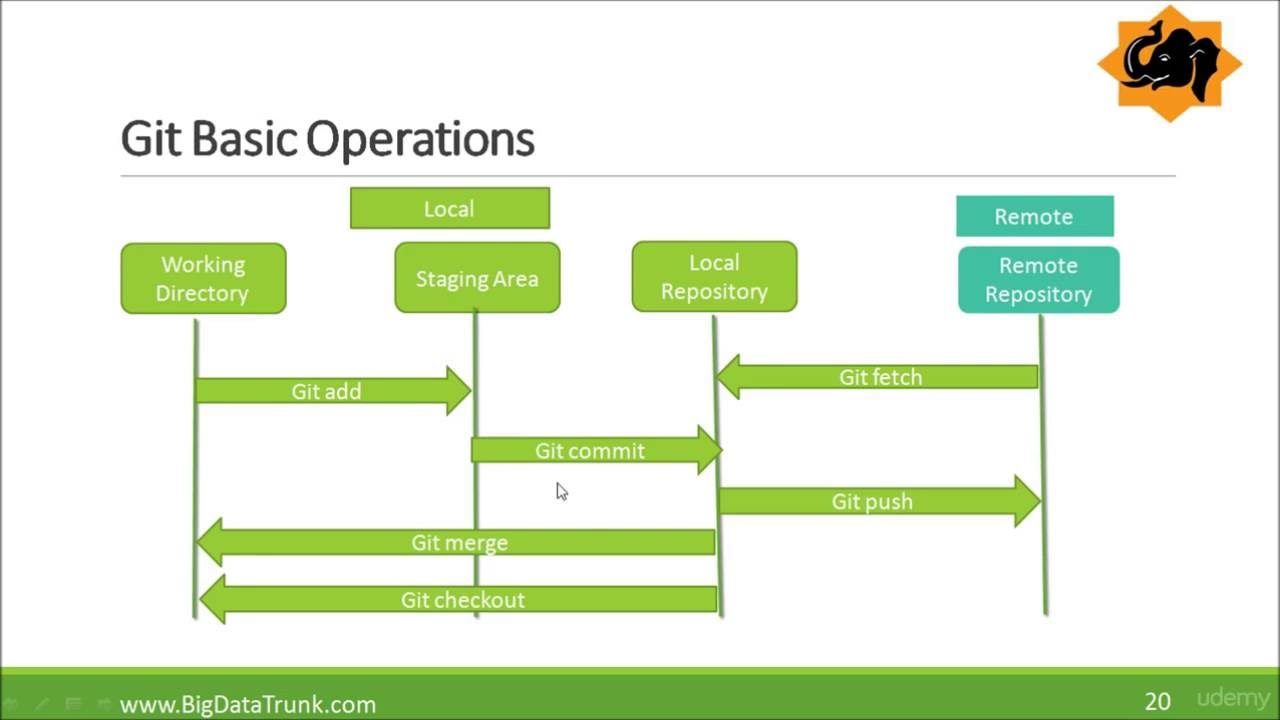
\includegraphics[width=10cm,height=7cm]{Figures/dapgit4.jpg}
\begin{equation}Alur Git \end{equation}

\subsection{Pengertian Lanjutan}

Mungkin sudah terlalu sering kita bekerja mandiri pada project pribadi, disini saya akan menunjukkan bagaimana caranya berkontribusi di project lain. Hal termudah untuk mencapai itu kita cari proyek open sources, apa itu proyek opensources, Proyek perangkat lunak open source merupakan proyek yang memberikan kode program kepada penggunanya secara bebas, dan tak jarang pengembangannya dilakukan secara terbuka: siapapun boleh berkontribusi dalam menulis kode tersebut. Menggunakan perangkat lunak open source tentunya sangat baik, karena selain tidak melakukan pembajakan, kita juga mendukung para pengembang dari perangkat lunak yang kita gunakan. Tetapi, akan lebih baik lagi jika kita juga ikut berkontribusi, mulai dari kontribusi pengunaan, pelaporan bug, sampai dengan kontribusi kode. Kontribusi pada proyek open source akan membantu kita untuk meningkatkan kemampuan pengembangan perangkat lunak.". \par
\vspace{12pt}
\vspace{12pt}
\noindent 
\section{Welcome Contributors} \par
Fork it! \par
Create your feature branch: git checkout -b my-new-feature \par
Commit your changes: git commit -am 'Add some feature' \par
Push to the branch: git push origin my-new-feature \par
Submit a pull request ;) \par
\noindent 
Tahapan berkontribusi yang baik, \par
\noindent 
Cari proyek opensources. \textit{(disini saya sebagai pengembang android saya akan memberikan contoh cara berkontribusi di salah satu proyek opensources pada library android)} \par
\noindent 
\section{Material Tabs} \par
\noindent 
Coba cari cari info tentang aturan kontribusi atau bisa dengan cara melakukan pendekatan pada developer terkait baik via email atau sosial akun. \par
\noindent 
Jika memang telah melakukan pendekatan atau tidak ada jalur lain untuk menempuh jalan tersebut, anda bisa langsung saja untuk melakukan fork project yang akan berkontribusi di dalamnya dimana nantinya kode akan di review oleh pemilik repository untuk di gabungkan atau tidaknya. \par
\noindent 
Setelah selesai fork, maka repository akan masuk ke list repo milik anda, untuk selanjutnya mungkin langsung saja, kali ini masuk pada git command apa aja yang bisa kita gunakan untuk berkontribusi di proyek opensources beserta simulasi yang akan saya contoh kan untuk berkontribusi pada proyek library android - material tabs . \par
\vspace{12pt}
\noindent 
git --help to see another commands cloning project yang suda anda fork ke akun anda \par
\vspace{12pt}
\noindent 
it clone git@github.com:CreatorB/MaterialTabs.git \par
\noindent 
untuk memudahkan development, hendaknya kita menambahkan repository pusat dengan lokal milik kita agar tidak terjadi konflik dengan kontributor lainnya. git remote add <nama-repo> <alamat-repo> \par
\noindent 
git remote add upstream git://github.com/neokree/MaterialTabs.git \par
\noindent 
Setelah remote repositori selesai dan seperti yang saya katakan tadi agar kita tidak hanya asal berkontribusi tapi memang benar benar clear dalam membantu development maka kita hendaknya juga membuat branch baru terlebih dahulu agar tidak merusak history dan nantinya juga akan memudahkan untuk racking code. git checkout -b <nama-cabang> \par
\noindent 
git checkout -b sample-project \par
\noindent 
Okkay sekarang setelah remote dan cabang / branch dibuat maka di cabang baru ini lah kita akan untuk melakukan perubahan kode yang nantinya bisa kita push ke repo pusat. Untuk berpindah branch bisa kita gunakan . git checkout <nama-cabang> dimana di repo lokal saya sekarang ada dua cabang cabang pertama adalah master dan cabang kedua adalah sample-project dan di sample-project saya bisa melakukan banyak perubahan kode. Jika memang ada penambahan file bisa menggunakan git add <nama-file-baru> atau kalo memang banyak file yang ditambahkan dan males add satu per satu, anda bisa langsung menuju root dari repository lalu git add . ya dot / titik berarti menambahkan semua perubahan yang ada di direktori tersebut secara rekursif. Setalah selesai perubahan silahkan lakukan commit, berisi pesan apa yang telah anda kontribusikan / lakukan perubahan. \par
\noindent 
git commit -m "fixing sample project and compile gradle added" \par
\noindent 
Setelah selesai melakukan commit, kita lakukan persiapan untuk pull ke repo pusat, sebelum itu kita pindah branch dulu ke master. \par
\noindent 
git checkout master \par
\noindent 
Setelah itu, kita akan mengambil kode lagi dari pusat, untuk memastikan tidak terdapat konflik pada kontribusi kode kita. Konflik dapat terjadi jika dua atau lebih kontributor melakukan perubahan pada satu berkas, terutama jika perubahan dilakukan pada baris yang sama, terlepas dari apakah tujuan perubahan sama atau tidak. Perintah yang digunakan adalah git fetch dan git merge pada cabang utama. \par
\noindent 
git fetch upstream \par
\noindent 
Setelah fetching selesai, sekarang kita merge dengan master. \par
\noindent 
git merge upstream/master \par
\noindent 
Dengan beberapa proses diatas, setidaknya kita telah bisa memastikan bahwanya tidak ada konflik dengan repo pusat. Sekarang kita kembali ke branch lokal development saya . sample-project \par
\noindent 
git checkout sample-project \par
\noindent 
dan menggabungkan cabang tersebut dengan cabang utama, sehingga kontribusi dapat dikirimkan kembali ke repositori pusat milik neokree, Material Tabs android library, dengan perintah git rebase <nama-branch> \par
\noindent 
git rebase master \par
\noindent 
Sebelum push ke repositori pusat milik neokree, maka terlebih dahulu akan saya push ke repository milik saya hasil fork di awal pembahasan tadi, dimana banyak perubahan yang dilakukan di branch tersebut. \par
\noindent 
git push origin sample-project \par
\noindent 
Setelah di push maka sekarang kita pergi menuju browser untuk melakukan pull request, cek / compare perubahan apa yang telah anda lakukan di branch anda pada branch master milik repo pusat, dan anda juga bisa menyisipkan pesan untuk memberitahukan developer pemilik repo pusat tentang apa yang anda lakukan, setelah yakin terhadap perubahan yang telah anda lakukan silahkan pilih create pull request dan selamat menunggu pemilik repo pusat untuk menanggapi di terima tidaknya kontribusi anda. \par
\vspace{12pt}
\noindent 
\textbf{Cara Push} \par
\vspace{12pt}
\noindent 
Pada dasarnya Git merupakan source control yang berbasis command line, akan tetapi berbagai macam aplikasi GUI Tools sudah banyak di jumpai agar dapat memudahkan kita dalam proses pengerjaan sebuah project atau mempermudah kita yang tidak terlalu mahir dalam penggunaan syntax-syntax tersebut, salah satunya itu SourceTree ini.\vspace{\baselineskip}
\vspace{\baselineskip}
Langsung saja saya mulai untuk proses yang ingin saya contohkan yaitu cara push, pull, commit project ke github dengan menggunakan aplikasi SourceTree. Lalu apa saja yang perlu dipersiapkan ? Berikut adalah beberapa yang perlu anda persiapkan untuk memulai peroses. \par
\noindent 
1 install aplikasi gitbash \par
\noindent 
Bagi~anda yang belum memiliki aplikasi SourceTree, anda dapat men-download nya pada web resmi yang sudah disediakan oleh pengembang aplikasi SourceTree. Aplikasi ini gratis, benar-banar gratis untuk berbagai macam keperluan komersial atau non-komersial. Anda dapat men-download nya pada  web dari githu \par
\noindent 
2~ Akun Github \par
\noindent 
Pastikan anda sudah memiliki akun Github, jika belum memilikinya anda dapat membuatnya terlebih dahulu dengan melakukan register terlebih dahulu, $  $https://github.com/ $  $atau~lihat tutorial cara mendaftar akun Github  Lalu kemudian anda login pada akun Github nya. \par
\vspace{12pt}
\noindent 
Jika sumua keperluan diatas sudah anda siapkan, sekarang kita mulai masuk pada tutorial, ikuti contoh dan prosesnya seperti dibawah ini : \par
\vspace{12pt}
\noindent 
Pertama yang harus anda lakukan adalah untuk menyimpan data-data project pada Github, terlebih dahulu anda membuat repository. Caranya anda klik tanda $  $\textbf{+} pada bagian kanan-atas lalu pilih "\textbf{New Repository}" Lalu anda buat nama untuk repositorinya, lalu klik "Create Repository"  \par
\vspace{12pt}
\noindent 
Setelah itu buka aplikasi SourceTree, jika sudah terbuka aplikasinya maka tampilannya akan seperti gambar dibawh ini. *Pastikan anda sudah login aplikasi SourceTree nya dengan menggunakan akun Github yang anda sudah buat. \par
\vspace{12pt}
\noindent 
repository yang kita buat caranya adalah klik browse pada gambar \textbf{"bumi"}, maka akan tampil semua repository yang kita sudah pernah buat, lalu pilih salah satu repository. Kemudian pada bagian \textbf{Destination Path : }itu adalah lokasi penyimpanan lokal yang kita ingin tempatkan.\vspace{\baselineskip}
\vspace{\baselineskip}
Harus anda ingat lokasi penyimpanan lokal anda, karena ketika kita akan melakukan pull, push, commit dilakukan pada penyimpanan lokal tersebut. Jiak sudah klik \textbf{Clone}. \par
\noindent 
Melakukan Proses Commit  $  \&  $ Push \par
\vspace{12pt}
\noindent 
Kemudian anda buka folder lokal kalian, lalu pindahkan dan letakkan semua file project kalian folder lokal kalian. Saya berikan contoh meletakkan satu file kedalam folder lokal, lihat seperti contoh gambar dibawah ini. \par
\vspace{12pt}
\noindent 
Kemudian anda buka folder lokal kalian, lalu pindahkan dan letakkan semua file project kalian folder lokal kalian. \par
\vspace{12pt}
\noindent 
Lalu anda simpan file yang sudah dibuat, sekarang kembali ke aplikasi SourceTree ketika ada file baru yang di letakkan pada folder lokal maka akan terdeteksi pada aplikasi SourceTree \par
\vspace{12pt}
\noindent 
Kemudian anda pindahkan file yang tadi sudah dibuat menjadi keatas dengan cara klik button \textbf{"Stage All"} $  $kemudian anda isikan komentar yang anda inginkan. Jika sudah anda lakukan Commit, tunggu beberapa saat hingga proses selesai. \par
\vspace{12pt}
\noindent 
Jika sudah maka pada bagian menu \textbf{Push }diatas terdapat notifikasi angka 1 itu artinya ada satu file yang sudah siap di kirim pada server Github. Lalu anda klik menu \textbf{Push} $  $tersebut sehingga muncul \textit{dialog box }lalu anda klik button \textbf{Push} $  $tunggu beberapa saat hingga proses upload selesai. Jika sudah selesai anda bisa cek pada Github, apakah sudah masuk apa belum. \par
\vspace{12pt}
\noindent 
Sampai disini proses commit dan push sudah selesai dilakukan, Kemudian kita akan mencoba melakukan pull, yakni menarik/mengambil file yang ada pada repository. Terlebih dahulu anda membuat file baru pada Github untuk mencoba menarik/mengambil file yang telah dibuat pada repository ke dalam folder lokal. Caranya adalah dengan menekan tombol menu \textbf{Pull}. Kemudian akan muncul \textit{dialog box} Kemudian klik \textbf{OK.} \par
\vspace{12pt}
\noindent 
Tunggu beberapa saat hingga proses selesai dilakukan, jika proses sudah selesai sekarang cek pada folder lokal anda apakah file yang di tarik tadi sudah masuk atau belum. \par
\vspace{12pt}
\vspace{12pt}
\noindent 
Atau jika cara diatas tidak berhasil anda gunakan maka bisa menggunakan cara berikut ini meggunakan gitbash \par
\vspace{12pt}
\noindent 
Setelah kita mempunya akun GitHub dan mengistall software git maka kita bisa langsung meng upload project kita. \par
\noindent 
Buatlah repository di GitHub dengan mengklik icon repo "Create new repository". \par
\noindent 
Kemudian beri nama repository nya lalu beri deskripsi untuk repository yang kita buat jika perlu, kemudian setting public/private, kalau public berarti bisa di akses oleh semua orang, kemudian centang "initialize this repository with a README" dan tambahkan kategori repository jila perlu. \par
\noindent 
kemudian klik "create repository". \par
\noindent 
Jika repository berhasil dibuat, anda akan di berikan kunci akases berupa HTTP/SSH, ini yang akan kita gunakan untuk remote repository dari software GIT. Misal saya punya kunci HTTP http://github.com/acchoblues/APeK.git \par
\noindent 
\begin{enumerate}
\item Setelah anda berhasil membiat repository sekarang klik kanan pada folder project yang akan di upload. \par
\noindent 
\item Klik kanan pada project klik "Git Bash". \par
\noindent 
\item Kemudian akan muncul command prompt / CMD \par
\noindent 
\item Jika anda baru pertama kali meggunakan software GIT, sebaiknya konfigurasi username dan email dulu. \par
\noindent 
\end {enumerate}
Ketik \par
\noindent 

\begin{verbatim}
Git config --global user.name "username anda"  \par
\noindent 
Git config --global user.email isi $ 
 \_  $dengan $  \_  $email $ 
  \_  $anda@ymail.com  \par
\noindent 
\end{verbatim}
Setelah melakukan konfigurasi username dan email, sekarang kita lakukan inisiasi, ketikan  \par
\noindent 
Git init  \par
\noindent 
Kemudian kita tambahkan semua file yang ada dalam folder project kita, ketikan  \par
\noindent 
Git add *  \par
\noindent 
Kemudian kita buat commit project nya, misal disini saya kasih commit  $ " $versi 1.0.0 $ " $ , ketikan  \par
\noindent 
Git commit –m "versi 1.0.0"  \par
\noindent 
Setelah kita buat commit untuk project nya, sekarang kita remote repository yang kita buat tadi, tentunya kita menggunakan kunci HTTP yang ada pada repository tadi, kalo ane kan tadi contoh nya http://github.com/acchoblues/APeK.git , ketikan \par
\noindent 
Git remote add origin http://github.com/acchoblues/APeK.git  \par
\noindent 
Setelah me-remote repository kita tadi, sekarang kita pull project nya, ketikan  \par
\noindent 
Git pull origin master  \par
\noindent 
Terakhir kita kirim project kita ke repository kita, ketikan  \par
\noindent 
Git push origin master  \par
\noindent 
Biasanya ketika kita ketikan perintah push ini, kita akan diminta username dan password kita dan perlu di perhatikan untuk password nya biasa nya ketika kita mengetikan password maka pada command prompt nya tidak ditampilkan karakter apapun. \par
\noindent 
So jangan khawatir tunggu sampai selesai di upload projectnya. \par
\noindent 
kalau sudah selesai proses uploadnya silahkan refresh repository anda, insya allah jika sesuai dengan instruksi di atas maka project anda sudah terupload disana. \par
\vspace{12pt}
\vspace{12pt}

 
\begin{verbatim}

 $  \$  $ \textbf{git init --bare proyekKhadapi} \par

Initialized empty Git repository in F:/proyekkhadpi/ \par

\end{verbatim}
Perintah di atas akan membuat sebuah \textit{bare repository} yang hanya dipakai untuk melakukan sinkronisasi antara pekerjaan Edi dan Bram nantinya. \par
\vspace{12pt}
\noindent 
Di komputer Edi, berbekal dengan flash disk yang mengandung \textit{bare repository} tersebut, ia akan melakukan men-kloning \textit{repository} tersebut dengan memberikan perintah berikut ini: \par
\noindent 
 $  \$  $ \textbf{cd  $  \sim  $/Desktop} \par
\noindent 
\noindent 
\vspace{12pt}
\noindent 
\vspace{12pt}
\noindent 
Sekarang, di folder\textit{  $  \sim  $/Desktop} akan ada sebuah folder \textit{proyek}\textit{Khadapi} yang merupakan kloningan dari yang ada di flash disk. $  $ $  $ Edi hanya perlu meletakkan kode programnya di folder komputer tersebut, dan bukan di \textit{bare repository} di flash disk. \par
\vspace{12pt}
\noindent 
Bram kemudian meminjam flash disk berisi \textit{bare repository} tersebut, dan memberikan perintah yang sama untuk membuat kloning dari \textit{bare repository} yang ada di flash disk ke desktop-nya. \par
\vspace{12pt}
\noindent 
Kedua developer tersebut kemudian bekerja di komputer masing-masing. $  $ $  $ Sebagai contoh, ini adalah simulasi pekerjaan yang dilakukan oleh Edi di repository miliknya: \par
\noindent 
\begin{verbatim}


{echo 'Menu 1' >> menu.txt} \par
 
{echo 'Isi modul 1' >> modul1.txt} \par

{git add .} \par

{git commit -m 'Membuat modul 1'} \par

\end{verbatim}
Edi membuat dua file dengan nama \textit{menu.txt} dan \textit{modul1.txt}. $  $ $  $ Anggap saja ini adalah kode program  \par
\noindent 
Pada saat yang bersamaan, Bram juga menambahkan file pada repository miliknya: \par
\vspace{12pt}
\noindent 
 $  \$  $ \textbf{echo 'Menu 2' >> menu.txt} \par
\noindent 
 $  \$  $ \textbf{echo 'Isi modul 2' >> modul2.txt} \par
\noindent 
 $  \$  $ \textbf{git add .} \par
\noindent 
 $  \$  $ \textbf{git commit -m 'Membuat modul 2'} \par
\noindent 
\vspace{12pt}
\noindent 
Setelah semuanya selesai, Bram men-\textit{push} perubahan yang dilakukannya ke \textit{upstream} di flash disk. $  $ $  $ Ia memberikan perintah berikut ini: \par
\vspace{12pt}
\noindent 
 $  \$  $ \textbf{git push origin master} \par
\noindent 
\vspace{12pt}
\noindent 
Sekarang, commit dengan pesan ‘Membuat modul 2’ milik Bram sudah dipindahkan ke \textit{upstream }di flash disk. $  $ $  $ Untuk memastikannya, ia berpindah ke folder di flash disk, dan memberikan perintah berikut ini: \par
\vspace{12pt}
\noindent 
 $  \$  $ \textbf{cd F:/proyek}\textbf{Khadapi} \par
\noindent 
 $  \$  $ \textbf{git show-branch} \par
\noindent 
[master] Membuat modul 2 \par
\noindent 
\vspace{12pt}
\noindent 
Tugas Bram sudah selesai, $  $ ia kemudian menyerahkan flash disk yang berisi \textit{bare repository} ke Edi. $  $ $  $ Kebetulan Edi juga telah selesai mengerjakan modul 1, sehingga ia berniat men-\textit{push} perubahannya ke \textit{upstream}. $  $ $  $ Akan tetapi Edi akan memperoleh pesan kesalahan seperti berikut ini: \par
\vspace{12pt}
\noindent 
 $  \$  $ \textbf{git push origin master} \par
\noindent 
To file://F:/proyekKhadapi \par
\noindent 
~!~[reject]~~~~   master -> master (fetch first) \par
\noindent 
error: failed to push some refs to 'file://F:/proyekKhadapi' \par
\noindent 
\vspace{12pt}
\noindent 
Pesan kesalahan ini muncul karena pada saat Edi mengerjakan modul 1, $  $ Bram telah duluan men-\textit{push} kode programnya ke \textit{upstream }di flash disk. $  $ $  $ Agar bisa men-\textit{push} ke \textit{upstream}, Edi perlu terlebih dahulu mengambil perubahan yang dibuat oleh Bram di \textit{upstream} dan men-\textit{merge} perubahan tersebut dengan perubahan miliknya. $  $ $  $ Edi memberikan perintah berikut ini: \par
\vspace{12pt}
\noindent 
 $  \$  $ \textbf{git pull} \par
\noindent 
... \par
\noindent 
Auto-merging menu.txt \par
\noindent 
CONFLICT (add/add): Merge conflict in menu.txt \par
\noindent 
Automatic merge failed; fix conflicts and then commit the result. \par
\noindent 
\vspace{12pt}
\noindent 
\vspace{12pt}
\noindent 
Git biasanya cukup pintar dalam melakukan merging file yang konflik. $  $ $  $ Tapi pada kasus ini, baik Edi dan Bram sama-sama menambah item baru pada baris pertama, sehingga Git tidak tahu mana yang harus dipakai. $  $ $  $ Edi perlu memperbaiki konflik ini dengan mengubah file \textit{menu.txt} secara manual menjadi seperti berikut ini: \par
\vspace{12pt}
\vspace{12pt}
\noindent 
Menu 1 \par
\noindent 
Menu 2 \par
\noindent 
\vspace{12pt}
\noindent 
\vspace{12pt}
\noindent 
Setelah itu, Edi akan men-\textit{commit} perubahan ini dengan memberikan perintah berikut ini: \par
\vspace{12pt}
\noindent 
 $  \$  $ \textbf{git add menu.txt} \par
\noindent 
 $  \$  $ \textbf{git commit -m 'Menyesuaikan dengan perubahan dari Bram'} \par
\noindent 
\vspace{12pt}
\noindent 
Sekarang, Edi akan memiliki 3 file, yaitu \textit{menu.txt}, \textit{modul1.txt} dan \textit{modul2.txt.} $  $ $  $ Ini mewakili hasil akhir yang diharapkan. $  $ $  $ Untuk melihat riwayat perubahan, Edi dapat memberikan perintah berikut ini: \par
\noindent 
 $  \$  $ \textbf{git log} \par
\noindent 
commit 8ce2a6bdc83387c2f81c56d60e06fa0ce62a3df8 \par
\noindent 
Merge: 1bcc42b 841b46d \par
\noindent 
Author: Edi <edi@dev.com> \par
\noindent 
Date:~~ Fri Apr 12 06:19:25 2013 +0700 \par
\noindent 
\vspace{12pt}
\noindent 
~~~ Menyesuaikan dengan perubahan dari Bram \par
\noindent 
\vspace{12pt}
\noindent 
commit 841b46d0dea229f55fd215e9cfadcd58b8aa64c2 \par
\noindent 
Author: Bram <bram@dev.com> \par
\noindent 
Date:~~ Fri Apr 11 05:57:37 2013 +0700 \par
\noindent 
\vspace{12pt}
\noindent 
~~~ Membuat modul 2 \par
\noindent 
\vspace{12pt}
\noindent 
commit 1bcc42b2346b95830bd6b3363425a9c8fa3a92f4 \par
\noindent 
Author: Edi <edi@dev.com> \par
\noindent 
Date:~~ Fri Apr 10 05:56:45 2013 +0700 \par
\noindent 
\vspace{12pt}
\noindent 
~~~ Membuat modul 1 \par
\noindent 
\vspace{12pt}
\noindent 
Saat ini perubahan masih ada di repository lokal milik Edi. $  $ $  $ Untuk memindahkan perubahan ke \textit{upstream} yang ada di flash disk, Edi memberikan perintah berikut ini: \par
\vspace{12pt}
\noindent 
 $  \$  $ \textbf{git push} \par
\noindent 
Oke, Edi kemudian  \par
\noindent 
meninggalkan komputer dan menikmati hidupnya untuk sejenak. \par
\noindent 
Kita kembali lagi ke Bram. $  $ Saat ini Bram hanya memiliki kode program modul 2 dan tidak memiliki kode program modul 1 yang dibuat Edi. Bram juga ingin memperoleh kode program terbaru! $  $ Ia meminjam flash disk yang berisi \textit{bare repository}, mencolokkannya di komputer rumahnya, lalu Bram memberikan perintah berikut ini: \par
\vspace{12pt}
\noindent 
 $  \$  $ \textbf{git pull} \par
\noindent 
... \par
\noindent 
Updating 841b46d..8ce2a6b \par
\noindent 
Fast-forward \par
\noindent 
~menu.txt~   $  \vert  $ 1 + \par
\noindent 
 modul1.txt  $  \vert  $ 1 + \par
\noindent 
 2 files changed, 2 insertions(+) \par
\noindent 
 create mode 100644 modul1.txt \par
\noindent 
\vspace{12pt}
\noindent 
\vspace{12pt}
\noindent 
\vspace{12pt}
\noindent 
Kali ini tidak ada konflik saat melakukan \textit{pull} dari \textit{upstream}. $  $ $  $ Hal ini karena Edi sudah menyelesaikan (atau mengatasi) konflik tersebut sebelumnya. $  $ $  $ Sampai pada tahap ini, isi repository Bram akan sama persis dengan milik Edi (terdiri atas 3 file yaitu \textit{menu.txt}, \textit{modul1.txt} dan \textit{modul2.txt}). \par
\vspace{12pt}
\noindent 
Pada contoh ini, Bram dan Edi memakai \textit{bare repository} yang disimpan di sebuah flash disk sebagai perantara. $  $ $  $ Hal ini bukanlah sesuatu yang efisien terutama bila mereka dipisahkan oleh jarak yang jauh. $  $ $  $ Bila komputer mereka sama-sama terkoneksi ke internet, mereka dapat men-\textit{setup} sebuah server Git sebagai \textit{upstream}. $  $ $  $ Selain mendukung protokol git (\textit{native}), Git juga mendukung protokol lainnya seperti HTTP, HTTPS, SSH, dan SCP. $  $ $  $ Sebuah server Git paling mudah dikonfigurasi bila memakai sistem operasi Linux. $  $ $  $ Bila tidak ingin repot-report men-setup server sendiri, Bram dan Edit dapat layanan dari pihak penyedia server seperti GitHub. \par
\vspace{12pt}



\chapter{Update Operation}
\ref{git.jpg}:
\begin{figure}[ht]
	\centerline{
\includegraphics[width=10cm,height=7cm]{Figures/git.jpg}}
	\caption{learn git}
	\label{git.jpg}
\end{figure}

Git adalah version control system yang digunakan para developer untuk 
mengembangkan software secara bersama-bersama. Fungsi utama git yaitu 
mengatur versi dari source code program anda dengan mengasih tanda baris 
dan code mana yang ditambah atau diganti.
\vspace{12pt}

Git ini sebenernya memudahkan programmer untuk mengetahui perubahan 
source codenya daripada harus membuat file baru seperti Program.java, 
ProgramRevisi.java, ProgramRevisi2.java, ProgramFix.java. Selain itu, 
dengan git kita tak perlu khawatir code yang kita kerjakan bentrok, 
karena setiap developer bias membuat branch sebagai workspacenya.Fitur 
yang tak kalah keren lagi, pada git kita bisa memberi komentar pada 
source code yang telah ditambah/diubah, hal ini mempermudah developer 
lain untuk tahu kendala apa yang dialami developer lain.
\vspace{12pt}
Untuk mengetahui bagaimana menggunakan git, berikut perintah-perintah 
dasar git:

\newcounter{numberedCntE}
\begin{enumerate}
\item Git init : untuk membuat repository pada file lokal yang nantinya 
ada folder .git
\item Git status : untuk mengetahui status dari repository lokal
\item Git add : menambahkan file baru pada repository yang dipilih
\item Git commit : untuk menyimpan perubahan yang dilakukan, tetapi 
tidak ada perubahan pada remote repository.
\item Git push : untuk mengirimkan perubahan file setelah di commit ke 
remote repository.
\item Git branch : melihat seluruh branch yang ada pada repository
\item Git checkout : menukar branch yang aktif dengan branchyang dipilih
\item GIt merge : untuk menggabungkan branch yang aktif dan branch yang 
dipilih
\item Git clone : membuat Salinan repository lokal
\setcounter{numberedCntE}{\theenumi}
\end{enumerate}
Contoh dari software version control system adalah github, bitbucket, 
snowy evening, dan masih banyak lagi. Jika anda sebagai developer belum 
mengetahui fitur git ini, maka anda wajib mencoba dan memakainya. Karena 
banyak manfaat yang akan didapat dengan git ini.
\vspace{12pt}

Dalam melakukan pemrograman, perubahan spesifikasi atau kebutuhan adalah 
hal yang tidak dapat dihindari. Tidak ada program yang dapat dituliskan 
dengan sempurna pada percobaan pertama. Hal ini menyebabkan pengembang 
perangkat lunak sangat dekat dengan sistem kontrol versi, baik secara 
manual maupun menggunakan perangkat lunak khusus. Seri tulisan ini akan 
membahas tentang sistem kontrol versi, kegunaannya, serta contoh kasus 
menggunakan git, salah satu perangkat lunak populer untuk kontrol versi.

\section{Dasar Kontrol Versi}

Kegunaan utama dari sistem kontrol versi ialah sebagai alat untuk 
manajemen kode program. Terdapat dua kegunaan utama dari sistem ini, 
yaitu:

\newcounter{numberedCntC}
\begin{enumerate}
\item Menyimpan versi lama dari kode, maupun
\item Menggabungkan perubahan-perubahan kode dari versi lama (misal: 
untuk mengembalikan fitur yang telah dihapus) ataupun menggabungkan 
perubahan dari orang lain (misal: menggabungkan fitur yang dikembangkan 
oleh anggota tim lain).
\setcounter{numberedCntC}{\theenumi}
\end{enumerate}
Tanpa menggunakan sistem kontrol versi, yang sering saya temukan (dan 
dulunya saya gunakan, sebelum mengetahui tentang kontrol versi) ialah 
pengunaan direktori untuk memisahkan beberapa versi program.
\vspace{12pt}
Sistem kontrol versi, seperti git, hg, atau bzr, dikembangkan untuk 
menyelesaikan masalah-masalah di atas. Karena tidak ingin membahas 
terlalu banyak, artikel ini hanya akan menjelaskan pengunaan git, karena 
kelihatannya git merupakan perangkat lunak kontrol versi yang paling 
populer untuk sekarang (mengingat popularitas Github dan pengunaan git 
pada kernel Linux).
\vspace{12pt}


\subsection{Git}

Git adalah sebuah perangkat lunak untuk mengontrol versi sebuah 
perangkat lunak "VCS/Version Control System". Git diciptakan oleh Linux 
Torvalds, yang pada awalnya ditujukan untuk pengembangan kernel Linux. 
Saat ini banyak perangkat lunak yang terkenal menggunakan Git sebagai 
pengotrol revisinya.
\vspace{12pt}
Pada bab ini akan mempelajari bagaimana cara menggunakan Git seperti 
proses life cycle Git, operasi-operasi dasar dan bagaimana cara 
menangani masalah saat menggunakan Git.
\vspace{12pt}
Git menyimpan sementara perubahan yang telah di buat pada copy-an 
pekerjaan Anda sehingga Anda dapat mengerjakan sesuatu yang lain, lalu 
kembali dan terapkan kembali nanti. Stashing berguna jika Anda perlu 
mengubah konteks dan mengerjakan hal lain dengan lebih cepat, tapi Anda 
sedang melewati perubahan kode dan tidak cukup siap untuk melakukannya. 
\vspace{12pt}
Perintah git stash mengambil perubahan yang tidak terikat (baik yang 
dipasang maupun yang tidak terpasang), menyimpannya untuk penggunaan 
selanjutnya, lalu mengembalikannya dari salinan pekerjaan Anda. Sebagai 
contoh:
\vspace{12pt}
\begin{verbatim}

\$ git status

On branch master

Changes to be committed:

new file: style.css

Changes not staged for commit:

modified: index.html

\$ git stash

Saved working directory and index state WIP on master: 5002d47 our new 
homepage

HEAD is now at 5002d47 our new homepage

\$ git status

On branch master

nothing to commit, working tree clean
\end{verbatim}

Pada poin ini Anda bebas melakukan perubahan, membuat commit baru, 
mengganti cabang, dan melakukan operasi Git lainnya; Kemudian kembali 
dan pasang kembali simpanan Anda saat Anda siap.
\vspace{12pt}
\newcounter{numberedCntD}
\begin{enumerate}
\item Perhatikan bahwa simpanannya adalah lokal ke tempat penyimpanan 
Git Anda. 
\item Mengajukan kembali perubahan tersimpan Anda
\item Anda dapat mengajukan permohonan kembali sebelumnya menyimpan 
perubahan dengan git stash pop:
\setcounter{numberedCntD}{\theenumi}
\end{enumerate}

\begin{verbatim}
\$ git status

On branch master

nothing to commit, working tree clean

\$ git stash pop

On branch master

Changes to be committed:

new file: style.css

Changes not staged for commit:

modified: index.html

Dropped refs/stash@\{0\} (32b3aa1d185dfe6d57b3c3cc3b32cbf3e380cc6a)
\end{verbatim}

Memindahkan simpanan Anda akan menghilangkan perubahan dari simpanan 
Anda dan memasangnya kembali ke salinan pekerjaan Anda.



Sebagai alternatif, Anda dapat mengajukan permohonan kembali perubahan 
pada copy pekerjaan Anda dan menyimpannya di tempat penyimpanan dengan 
git stash berlaku:

\begin{verbatim}
\$ git stash apply

On branch master

Changes to be committed:

new file: style.css

Changes not staged for commit:

modified: index.html

\end{verbatim}


Ini berguna jika Anda ingin menerapkan perubahan tersimpan yang sama ke 
beberapa cabang.

Sekarang setelah Anda mengetahui dasar-dasar stashing, ada satu 
peringatan dengan penyimpanan git yang perlu Anda sadari: Secara default 
Git tidak akan menyimpan perubahan yang dibuat pada file yang tidak 
terlacak atau diabaikan.

\textbf{Menyembunyikan file yang tidak terlacak atau diabaikan}

Secara default, menjalankan git stash akan menyimpan:

\newcounter{numberedCntA}
\begin{enumerate}
\item perubahan yang telah ditambahkan ke indeks Anda (perubahan 
bertahap)
\item Perubahan yang dilakukan pada file yang saat ini dilacak oleh Git 
(perubahan yang tidak terhapus)
\setcounter{numberedCntA}{\theenumi}
\end{enumerate}
Tapi itu tidak akan disimpan:

\newcounter{numberedCntB}
\begin{enumerate}
\item file baru dalam copy pekerjaan Anda yang belum dipentaskan
\item file yang telah diabaikan
\setcounter{numberedCntB}{\theenumi}
\end{enumerate}
Jadi jika kita menambahkan file ketiga ke contoh kita di atas, tapi 
jangan tingkatkan (misal kita tidak menjalankan git add), git stash 
tidak akan menyimpannya.\vspace{12pt} 

\begin{verbatim}
\$ script.js

\$ git status

On branch master

Changes to be committed:

new file: style.css

Changes not staged for commit:

modified: index.html

Untracked files:

script.js

\$ git stash

Saved working directory and index state WIP on master: 5002d47 our new 
homepage

HEAD is now at 5002d47 our new homepage

\$ git status

On branch master

Untracked files:

script.js

\end{verbatim}

Menambahkan opsi -u (atau --include-unracked) memberitahu git stash 
untuk juga menyimpan file yang tidak terlacak.\vspace{12pt}



Jadi, sebenarnya apa yang dimaksud dengan Git? Ini adalah bagian penting 
untuk dipahami, karena jika anda memahami apa itu Git dan cara kerjanya, 
maka dapat dipastikan anda dapat menggunakan Git secara efektif dengan 
mudah. Selama mempelajari Git, cobalah untuk melupakan VCS lain yang 
mungkin telah anda kenal sebelumnya, misalnya Subversion dan Perforce. 
Git sangat berbeda dengan sistem-sistem tersebut dalam hal menyimpan dan 
memperlakukan informasi yang digunakan, walaupun antar-muka penggunanya 
hampir mirip. Dengan memahami perbedaan tersebut diharapkan dapat 
membantu anda menghindari kebingungan saat menggunakan Git.\vspace{12pt}

Salah satu perbedaan yang mencolok antar Git dengan VCS lainnya 
(Subversion dan kawan-kawan) adalah dalam cara Git memperlakukan 
datanya. Secara konseptual, kebanyakan sistem lain menyimpan informasi 
sebagai sebuah daftar perubahan berkas. Sistem seperti ini (CVS, 
Subversion, Bazaar, dan yang lainnya) memperlakukan informasi yang 
disimpannya sebagai sekumpulan berkas dan perubahan yang terjadi pada 
berkas-berkas tersebut.\vspace{12pt}

Git memperlakukan datanya sebagai sebuah kumpulan snapshot dari sebuah 
miniatur sistem berkas. Setiap kali anda melakukan commit, atau 
melakukan perubahan pada proyek Git anda, pada dasarnya Git merekam 
gambaran keadaan berkas-berkas anda pada saat itu dan menyimpan 
referensi untuk gambaran tersebut. Agar efisien, jika berkas tidak 
mengalami perubahan, Git tidak akan menyimpan berkas tersebut melainkan 
hanya pada file yang sama yang sebelumnya telah disimpan.\vspace{12pt}

Ini adalah sebuah perbedaan penting antara Git dengan hampir semua VCS 
lain. Hal ini membuat Git mempertimbangkan kembali hampir setiap aspek 
dari version control yang oleh kebanyakan sistem lainnya disalin dari 
generasi sebelumnya. Ini membuat Git lebih seperti sebuah miniatur 
sistem berkas dengan beberapa tool yang luar biasa ampuh yang dibangun 
di atasnya, ketimbang sekadar sebuah VCS. Kita akan mempelajari beberapa 
manfaat yang anda dapatkan dengan memikirkan data anda dengan cara ini 
ketika kita membahas "Git branching" pada Bab 3.\vspace{12pt}

\textbf{Hampir Semua Operasi Dilakukan Secara Lokal}\vspace{12pt}

Kebanyakan operasi pada Git hanya membutuhkan berkas-berkas dan resource 
lokal - tidak ada informasi yang dibutuhkan dari komputer lain pada 
jaringan anda. Jika Anda terbiasa dengan VCS terpusat dimana kebanyakan 
operasi memiliki overhead latensi jaringan, aspek Git satu ini akan 
membuat anda berpikir bahwa para dewa kecepatan telah memberkati Git 
dengan kekuatan. Karena anda memiliki seluruh sejarah dari proyek di 
lokal disk anda, dengan kebanyakan operasi yang tampak hampir seketika.\vspace{12pt}

Sebagai contoh, untuk melihat history dari proyek, Git tidak membutuhkan 
data histori dari server untuk kemudian menampilkannya untuk anda, namun 
secara sedarhana Git membaca historinya langsung dari basisdata lokal 
proyek tersebut. Ini berarti anda melihat histori proyek hampir secara 
instant. Jika anda ingin membandingkan perubahan pada sebuah berkas 
antara versi saat ini dengan versi sebulan yang lalu, Git dapat mencari 
berkas yang sama pada sebulan yang lalu dan melakukan pembandingan 
perubahan secara lokal, bukan dengan cara meminta remote server 
melakukannya atau meminta server mengirimkan berkas versi yang lebih 
lama kemudian membandingkannya secara lokal.\vspace{12pt}

Hal ini berarti bahwa sangat sedikit yang tidak bisa anda kerjakan jika 
anda sedang offline atau berada diluar VPN. Jika anda sedang berada 
dalam pesawat terbang atau sebuah kereta dan ingin melakukan pekerjaan 
kecil, anda dapat melakukan commit sampai anda memperoleh koneksi 
internet hingga anda dapat menguploadnya. Jika anda pulang ke rumah dan 
VPN client anda tidak bekerja dengan benar, anda tetap dapat bekerja. 
Pada kebanyakan sistem lainnya, melakukan hal ini cukup sulit atau 
bahkan tidak mungkin sama sekali. Pada Perforce misalnya, anda tidak 
dapat berbuat banyak ketika anda tidak terhubung dengan server; pada 
Subversion dan CVS, anda dapat mengubah berkas, tapi anda tidak dapat 
melakukan commit pada basisdata anda (karena anda tidak terhubung dengan 
basisdata). Hal ini mungkin saja bukanlah masalah yang besar, namun anda 
akan terkejut dengan perbedaan besar yang disebabkannya.\vspace{12pt}

\textbf{Git Memiliki Integritas}\vspace{12pt}

Segala sesuatu pada Git akan melalui proses checksum terlebih dahulu 
sebelum disimpan yang kemudian direferensikan oleh hasil checksum 
tersebut. Hal ini berarti tidak mungkin melakukan perubahan terhadap 
berkas manapun tanpa diketahui oleh Git. Fungsionalitas ini dimiliki 
oleh Git pada level terendahnya dan ini merupakan bagian tak terpisahkan 
dari filosofi Git. Anda tidak akan kehilangan informasi atau mendapatkan 
file yang cacat tanpa diketahui oleh Git.\vspace{12pt}

Mekanisme checksum yang digunakan oleh Git adalah SHA-1 hash. Ini 
merupakan sebuah susunan string yang terdiri dari 40 karakter 
heksadesimal (0 hingga 9 dan a hingga f) dan dihitung berdasarkan isi 
dari sebuah berkas atau struktur direktori pada Git.\vspace{12pt}

\subsubsection{Secara Umum Git Hanya Menambahkan Data}\vspace{12pt}
Ketika anda melakukan operasi pada Git, kebanyakan dari operasi tersebut 
hanya menambahkan data pada basisdata Git. It is very difficult to get 
the system to do anything that is not undoable or to make it erase data 
in any way. Seperti pada berbagai VCS, anda dapat kehilangan atau 
mengacaukan perubahan yang belum di-commit; namun jika anda melakukan 
commit pada Git, akan sangat sulit kehilanngannya, terutama jika anda 
secara teratur melakukan push basisdata anda pada repositori lain.\vspace{12pt}

Hal ini menjadikan Git menyenangkan karena kita dapat berexperimen tanpa 
kehawatiran untuk mengacaukan proyek. Untuk lebih jelas dan dalam lagi 
tentang bagaimana Git menyimpan datanya dan bagaimana anda dapat 
mengembalikan yang hilang, lihat "Under the Covers" pada Bab 9.\vspace{12pt}

\subsubsection{Tiga Keadaan}\vspace{12pt}
Sekarang perhatikan. Ini adalah hal utama yang harus diingat tentang Git 
jika anda ingin proses belajar anda berjalan lancar. Git memiliki 3 
keadaan utama dimana berkas anda dapat berada: committed, modified dan 
staged. Committed berarti data telah tersimpan secara aman pada 
basisdata lokal. Modified berarti anda telah melakukan perubahan pada 
berkas namun anda belum melakukan commit pada basisdata. Staged berarti 
anda telah menandai berkas yang telah diubah pada versi yang sedang 
berlangsung untuk kemudian dilakukan commit.\vspace{12pt}

Direktori Git adalah dimana Git menyimpan metadata dan database objek 
untuk projek anda. Ini adalah bahagian terpenting dari Git, dan inilah 
yang disalin ketika anda melakukan kloning sebuah repository dari 
komputer lain.\vspace{12pt}

Direktori kerja adalah sebuah checkout tunggal dari satu versi dari 
projek. Berkas-berkas ini kemudian ditarik keluar dari basisdata yang 
terkompresi dalam direktori Git dan disimpan pada disk untuk anda 
gunakan atau modifikasi.\vspace{12pt}

Staging area adalah sebuah berkas sederhana, umumnya berada dalam 
direktori Git anda, yang menyimpan informasi mengenai apa yang menjadi 
commit selanjutnya. Ini terkadang disebut sebagai index, tetapi semakin 
menjadi standard untuk menyebutnya sebagai staging area.\vspace{12pt}

\begin{table}[ht]
	\caption{Alur kerja dasar git}
	\centering
	\begin{tabular}{cccc}
		\hline
		No&Keterangan&\\
		\hline
		.1&Mengubah berkas dalam direktori kerja&\\
		.2&Menambahkan snapshotnya ke staging 
		area&\\
		.3&Commit,Ambil berkas di 
		staging area dan menyimpan snapshotnya ke direktori Git&\\
		\hline
	\end{tabular}
\end{table}

Jika sebuah versi tertentu dari sebuah berkas telah ada di direktori 
git, ia dianggap 'committed'. Jika berkas diubah (modified) tetapi sudah 
ditambahkan ke staging area, maka itu adalah 'staged'. Dan jika berkas 
telah diubah sejak terakhir dilakukan checked out tetapi belum 
ditambahkan ke staging area maka itu adalah 'modified'. Pada Bab 2, anda 
akan mempelajari lebih lanjut mengenai keadaan-keadaan ini dan bagaimana 
anda dapat memanfaatkan keadaan-keadaan tersebut ataupun melewatkan 
bagian 'staged' seluruhnya.\vspace{12pt}

\textbf{Modifikasi Fungsi yang Ada}\vspace{12pt}

Tom melakukan operasi kloning dan menemukan file baru string.c. Dia 
ingin tahu siapa yang menambahkan file ini ke repositori dan untuk 
tujuan apa, maka, dia menjalankan perintah git log.\vspace{12pt}

[$tom@CentOS ]~$ git clone gituser@git.server.com:project.git\vspace{12pt}

Perintah di atas akan menghasilkan hasil sebagai berikut:\vspace{12pt}

Initialized empty Git repository in /home/tom/project/.git/

remote: Counting objects: 6, done.

remote: Compressing objects: 100\% (4/4), done.

Receiving objects: 100\% (6/6), 726 bytes, done.

remote: Total 6 (delta 0), reused 0 (delta 0)\vspace{12pt}

Operasi Clone akan membuat direktori baru di dalam direktori kerja saat 
ini. Dia mengubah direktori ke direktori yang baru dibuat dan 
menjalankan perintah git log.\vspace{12pt}

[$tom@CentOS ~$] cd project/

[$tom@CentOS project ~$]git log\vspace{12pt}

Perintah di atas akan menghasilkan hasil sebagai berikut:\vspace{12pt}

commit d1e19d316224cddc437e3ed34ec3c931ad803958

Author: Jerry Mouse $<$jerry@tutorialspoint.com$>$

Date: Wed Sep 11 08:05:26 2013 +0530

Changed return type of my\_strlen to size\_t

commit 19ae20683fc460db7d127cf201a1429523b0e319

Author: Tom Cat $<$tom@tutorialspoint.com$>$

Date: Wed Sep 11 07:32:56 2013 +0530

Initial commit\vspace{12pt}

Setelah mengamati log, dia menyadari bahwa file string.c ditambahkan 
oleh Jerry untuk mengimplementasikan operasi string dasar. Dia penasaran 
dengan kode Jerry. Jadi dia membuka string.c di editor teks dan langsung 
menemukan bug. Dalam fungsi my\_strlen, Jerry tidak menggunakan pointer 
konstan. Jadi, dia memutuskan untuk memodifikasi kode Jerry. Setelah 
modifikasi, kode tersebut terlihat seperti berikut:\vspace{12pt}

$[$tom@CentOS project$]$\$ git diff\vspace{12pt}

Perintah di atas akan menghasilkan hasil sebagai berikut:\vspace{12pt}

diff --git a/string.c b/string.c

index 7da2992..32489eb 100644
\begin{equation}
--- a/string.c
\end{equation}

+++ b/string.c

@@ -1,8 +1,8 @@

\#include $<$stdio.h$>$

-size\_t my\_strlen(char *s)

+size\_t my\_strlen(const char *s)

\{

 - char *p = s;

 + const char *p = s;

 while (*p)

 ++p;

\}\vspace{12pt}

Setelah melakukan pengujian, dia menyimpan perubahannya.\vspace{12pt}
[$tom@CentOS project ~$] git status -s
M string.c
?? string

[$tom@CentOS project ~$] git add string.c

[$tom@CentOS project ~$] git commit -m 'Changed char pointer to const char pointer'
[master cea2c00] Changed char pointer to const char pointer
1 files changed, 2 insertions(+), 2 deletions(-)

[$tom@CentOS project ~$] git log\vspace{12pt}

perintah diatas akan menghasilkan hasil sebagai berikut:\vspace{12pt}

commit cea2c000f53ba99508c5959e3e12fff493b
Author: Tom Cat <tom@tutorialspoint.com>
Date: Wed Sep 11 08:32:07 2013 +0530

Changed char pointer to const char pointer


commit d1e19d316224cddc437e3ed34ec3c931ad803958

Author: Jerry Mouse $<$jerry@tutorialspoint.com$>$

Date: Wed Sep 11 08:05:26 2013 +0530

Changed return type of my\_strlen to size\_t

commit 19ae20683fc460db7d127cf201a1429523b0e319

Author: Tom Cat $<$tom@tutorialspoint.com$>$

Date: Wed Sep 11 07:32:56 2013 +0530

Initial commit\vspace{12pt}

Tom menggunakan git push untuk melakukan push atas perubahan yang dilakukannya.\par
\vspace{12pt}


[$tom@CentOS project ~$] git push origin master\par
\vspace{12pt}
perintah diatas akan menghasilkan seperti berikut:\par
\vspace{12pt}
Counting objects: 5, done.\par
\vspace{12pt}
Compressing objects: 100% (3/3), done.\par
\vspace{12pt}
Writing objects: 100% (3/3), 336 bytes, done.\par
\vspace{12pt}
Total 3 (delta 1), reused 0 (delta 0)\par
\vspace{12pt}
To gituser@git.server.com:project.git\par
\vspace{12pt}
d1e19d3..cea2c00 master −> master\par





\chapter{Stash Operation}
\section{Penjelasan}

Salah satu fitur menarik di Git adalah \textit{stashing}.�� Dengan 
melakukan\textit{stashing}, developer dapat dengan mudah '\textit{
melenyapkan}' perubahan kode program, melakukan perubahan lain, lalu 
kembali lagi ke kode program yang sebelumnya dikerjakan.�� 
Langkah-langkah tersebut sebenarnya dapat diwakili oleh beberapa 
perintah Git lainnya, tapi \textit{stashing}�membuatnya menjadi 
mudah karena hanya perlu memanggil satu perintah.\vspace{14pt}

Sebagai contoh, saya akan menggunakan Git yang diakses melalui IntelliJ 
IDEA.�� Saya membuat sebuah proyek Groovy baru dengan nama\textit{
latihan}.�� Lalu saya membuat sebuah script Groovy sederhana bernama
\textit{Latihan.groovy}untuk menghitung sisa inventory secara FIFO, 
seperti berikut ini:\vspace{14pt}


  List� pembelian = [10, 20, 30, 40]\par 
  List penjualan = [5, 6, 3, 2, 
1, 3]\par
 println stokFifo(pembelian, hitungTotal(pembelian, 
penjualan))\par�
 int hitungTotal(List pembelian, List penjualan) 
\{\par��
 pembelian.sum() - penjualan.sum()\}\par�
 List stokFifo(List pembelian, 
int sisa) \{\par����
 List hasil = []\par����
 pembelian.each \{ int jumlah 
->\par��������if (sisa $>$ 0) \{\par������������int delta = (jumlah $>$= 
sisa)? jumlah: sisa� // BUG YANG DISENGAJA!\par������������sisa -= 
delta\par������������hasil $<$$<$ delta\par��������\}\par����\}\par����hasil\par\} \vspace{14pt}

Untuk menambahkan proyek ke dalam repository Git, pilih menu VCS, Import into Version Control,Create Git Repository.\vspace{14pt}

Pada kotak dialog yang muncul, pilih untuk 
meletakkan�repository�bersamaan dengan lokasi proyek dan kemudian 
men-klik tombol�OK.\vspace{14pt}

Kemudian, klik kanan pada file�Latihan.groovy, memilih menu�Git,�Add\vspace{14pt}

Sekarang file tersebut telah berada di lokasi�index�atau�staging�dari 
Git.�� Berikutnya, commit perubahan.�� Caranya adalah 
dengan memilih menu�VCS,�Commit Changes.\vspace{14pt}

Pilih tombol Commit�untuk menyimpan perubahan dalam 
repository Git lokal.�� Saat IntelliJ IDEA memunculkan dialog mengenai 
file lain yang tidak ikut di-commit, pilih No.\vspace{14pt}

Anggap saja ini adalah sebuah aplikasi yang dikembangkan bersama dengan 
developer lain, yaitu xXx.�� xXx tersebut telah men-\textit{
fetch}�repository saya dari remote/upstream, kemudian ia akan 
men-develop kode program yang berhubungan dengan kode program saya di 
atas.\vspace{14pt}

Tentu saja saya juga tidak ingin ketinggalan sibuk.�� Saya menambahkan 
harga dan perhitungan laba pada kode program saya. saya menulis kode program berikut ini:
\begin{equation}
Map pembelian = [10: 10000, 20: 10100, 30: 10200, 40: 11000]
\end{equation}
\vspace{12pt}
Map penjualan = [5: 12000, 6: 13000, 3: 11000, 2: 11000, 1: 15000, 3: 12000]
println stokFifo(pembelian, 
hitungTotal(pembelian.keySet().toList(),
penjualan.keySet().toList()))\par�
int hitungTotal(List pembelian,
List
penjualan) {\par����pembelian.sum() - penjualan.sum()\par
}\par�
List stokFifo(Map 
pembelian, int sisa) {\par����List hasil = []\par����pembelian.each \{ 
jumlah, hargaBeli ->\par�������if (sisa > 0) {\par������������int delta = 
(jumlah >= sisa)? jumlah: sisa� // BUG YANG DISENGAJA!\par������������sisa 
-= delta\par������������hasil << [delta, 
hargaBeli]\par��������\}\par����\}\par����hasil\par \}\par�int hitungProfit(List stokFifo, Map penjualan)\par \vspace{14pt} 
Saya belum selesai mengetik, bahkan belum sempat menjalankan kode 
program ketika tiba-tiba telepon berdering.�� Suara xXx terdengar 
sangat panik.�� Dia mengatakan bahwa 30 menit lagi dirinya harus 
memberikan presentasi ke pengguna, tapi ada yang aneh dengan perhitungan 
inventory buatan saya!�� xXx menemukan sebuah kesalahan.� Lebih dari 
itu, xXx meminta saya untuk segera memperbaikinya secepat mungkin 
sehingga dia bisa men-pull perbaikan dari saya!\vspace{14pt}

Masalahnya: saya sudah mengubah banyak kode program tersebut sehingga 
tidak sama lagi seperti yang dipakai oleh Lena.�� Saya tidak ingin 
menghapus perubahan yang sudah saya buat sejauh ini karena nantinya 
perubahan ini pasti akan dipakai.\vspace{14pt}

Salah satu solusi yang dapat saya pakai adalah dengan memakai 
fasilitas�stashing�di Git.�� Saya memilih menu�VCS,�Git,�Stash Changes\vspace{14pt}

Setelah men-klik tombol Create Stash, isi kode program saya 
secara ajaib kembali lagi seperti semula!� Sama persis seperti commit 
terakhir yang dirujuk oleh HEAD.�� Saya segera memanfaatkan kesempatan 
ini untuk mencari dan memperbaiki kesalahan yang ditemukan xXx:\vspace{14pt}

 List� pembelian = $[$10, 20, 30, 40$]$List penjualan = $[$5, 6, 3, 2, 
1, 3$]$println stokFifo(pembelian, hitungTotal(pembelian, 
penjualan))�int hitungTotal(List pembelian, List penjualan) 
\{����pembelian.sum() - penjualan.sum()\}�List stokFifo(List pembelian, 
int sisa) \{����List hasil = $[$$]$����pembelian.each \{ int jumlah 
-$>$��������if (sisa $>$ 0) \{������������int delta = (jumlah $>$= 
sisa)? sisa: jumlah������������sisa -= delta������������hasil $<$$<$ 
delta��������\}����\}����hasil\}\vspace{14pt}

Saya segera men-commit perubahan dengan memilih menu\textbf{VCS},
\textbf{Commit Changes\ldots }.�� Pada komentar, saya mengisi dengan 
'Perbaikan perhitungan sisa inventory yang salah.' dan men-klik tombol
\textbf{Commit}.�� Saya kemudian men-\textit{push}�perubahan ke
\textit{upstream}, sehingga Lena bisa men-\textit{pull}�perubahan 
dari saya.�� Tidak lama kemudian suara Lena terdengar lega seolah-olah 
baru saja luput dari malapetaka.� Ia memberitahukan bahwa kini semuanya 
baik-baik saja.\vspace{14pt}

Lalu bagaimana dengan kode program yang sedang saya '\textit{ketik}' 
sebelum menerima telepon dari Lena?� Kemana perginya?�� Saya bisa 
mengembalikannya dengan memilih menu\textbf{VCS},\textbf{Git}
,\textbf{UnStash Changes\ldots }.�� Pada kotak dialog yang muncul, 
saya men-klik tombol\textbf{Pop Stash}\vspace{14pt}

Kode program saya akan kembali seperti terakhir kali:

 Map pembelian = $[$10: 10000, 20: 10100, 30: 10200, 40: 11000$]$Map 
penjualan = $[$5: 12000, 6: 13000, 3: 11000, 2: 11000, 1: 15000, 3: 
12000$]$println stokFifo(pembelian, 
hitungTotal(pembelian.keySet().toList(), 
penjualan.keySet().toList()))�int hitungTotal(List pembelian, List 
penjualan) \{����pembelian.sum() - penjualan.sum()\}�List stokFifo(Map 
pembelian, int sisa) \{����List hasil = $[$$]$����pembelian.each \{ 
jumlah, hargaBeli -$>$��������if (sisa $>$ 0) \{������������int delta = 
(jumlah $>$= sisa)? sisa: jumlah������������sisa -= 
delta������������hasil $<$$<$ $[$delta, 
hargaBeli$]$��������\}����\}����hasil\}�int hitungProfit(List stokFifo, 
Map penjualan) \{����def \\

Tunggu dulu!� Tidak persis sama seperti terakhir kali!!� Fasilitas
\textit{stashing}�bukan saja hanya mengembalikan kode program 
sebelumnya, tetapi juga melakukan merging dengan perubahan saat ini.�� 
Perbaikan yang diminta oleh Lena tidak hilang setelah saya men-pop 
stash.\vspace{14pt}

Pada contoh ini, hanya terdapat satu file yang berubah.�� Fasilitas 
stashing akan semakin berguna bila perubahan telah dilakukan pada banyak 
file yang berbeda.� Tanpa Git dan\textit{stashing}, pada kasus ini, 
saya harus memakai cara manual yang lebih repot seperti memberikan 
komentar atau mengedit file untuk sementara.\vspace{14pt}

\subsection{Membatalkan Apapun}

Pada setiap tahapan, Anda mungkin ingin membatalkan sesuatu. Di sini, 
kita akan membahas beberapa alat dasar untuk membatalkan perubahan yang 
baru saja Anda lakukan. Harus tetap diingat bahwa kita tidak selalu 
dapat membatalkan apa yang telah kita batalkan. Ini adalah salah satu 
area dalam Git yang dapat membuat Anda kehilangan apa yang telah Anda 
kerjakan jika Anda melakukannya dengan tidak tepat.\vspace{14pt}

\textbf{Merubah Commit Terakhir Anda}\vspace{14pt}

Salah satu pembatalan yang biasa dilakukan adalah ketika kita melakukan 
commit terlalu cepat dan mungkin terjadi lupa untuk menambah beberapa 
berkas, atau Anda salah memberikan pesan commit Anda. Jika Anda ingin 
untuk mengulang commit tersebut, Anda dapat menjalankan commit dengan 
opsi�--ammend:\vspace{14pt}

\$ git commit --amend\vspace{14pt}

Perintah ini mangambil area stage Anda dan menggunakannya untuk commit. 
Jika Anda tidak melakukan perubahan apapun sejak commit terakhir Anda 
(seumpama, Anda menjalankan perintah ini langsung setelah commit Anda 
sebelumnya), maka snapshot Anda akan sama persis dengan sebelumnya dan 
yang Anda dapat ubah hanyalah pesan commit Anda.\vspace{14pt}

Pengolah kata akan dijalankan untuk mengedit pesan commit yang telah 
Anda buat pada commit sebelumnya. Anda dapat ubah pesan commit ini 
seperti biasa, tetapi pesan commit sebelumnya akan tertimpa.\vspace{14pt}

Sebagai contoh, jika Anda melakukan commit dan menyadari bahwa Anda lupa 
untuk memasukkan beberapa perubahan dalam sebuah berkas ke area stage 
dan Anda ingin untuk menambahkan perubahan ini ke dalam commit terakhir, 
Anda dapat melakukannya sebagai berikut:\vspace{14pt}

\begin{verbatim}

\$ git commit -m 'initial commit'\vspace{14pt}

\$ git add forgotten\_file\vspace{14pt}

\$ git commit --amend\vspace{14pt}
\end{verbatim}

Ketiga perintah ini tetap akan bekerja di satu commit - commit kedua 
akan menggantikan hasil dari commit pertama.\vspace{14pt}

\textbf{Mengeluarkan Berkas dari Area Stage}\vspace{14pt}

Dua seksi berikutnya akan menunjukkan bagaimana menangani area stage 
Anda dan perubahan terhadap direktori kerja Anda. Sisi baiknya adalah 
perintah yang Anda gunakan untuk menentukan keadaan dari kedua area 
tersebut juga mengingatkan Anda bagaimana membatalkan perubahannya. 
Sebagai contoh, mari kita anggap Anda telah merubah dua berkas dan ingin 
melakukan commit kepada keduanya sebagai dua perubahan terpisah, tetapi 
Anda secara tidak sengaja mengetikkan�git add *�dan memasukkan keduanya 
ke dalam area stage. Bagaimana Anda dapat mengeluarkan salah satu dari 
keduanya? Perintah�git status�mengingatkan Anda:\vspace{14pt}

\$ git add\vspace{14pt}

\$ git status\vspace{14pt}

\# On branch master\vspace{14pt}

\# Changes to be committed:\vspace{14pt}

\# (use "git reset HEAD $<$file$>$..." to unstage)\vspace{14pt}

\#

\# modified: README.txt\vspace{14pt}

\# modified: benchmarks.rb\vspace{14pt}

\#

Tepat di bawah tulisan "Changes to be committed", tercantum anjuran 
untuk menggunakan�git reset HEAD $<$file$>$�untuk mengeluarkan dari area 
stage. Mari kita gunakan anjuran tersebut untuk mengeluarkan berkas 
benchmarks.rb dari area stage:\vspace{14pt}

\$ git reset HEAD benchmarks.rb 

benchmarks.rb: locally modified\vspace{14pt}

\$ git status\vspace{14pt}

\# On branch master\vspace{14pt}

\# Changes to be committed:\vspace{14pt}

\# (use "git reset HEAD $<$file$>$..." to unstage)\vspace{14pt}

\#

\# modified: README.txt\vspace{14pt}

\#

\# Changes not staged for commit:\vspace{14pt}

\# (use "git add $<$file$>$..." to update what will be committed)\vspace{14pt}

\# (use "git checkout -- $<$file$>$..." to discard changes in working 
directory)\vspace{14pt}

\#

\# modified: benchmarks.rb\vspace{14pt}

\#

Perintahnya terlihat agak aneh, tetapi menyelesaikan masalah. Berkas 
benchmarks.rb sekarang menjadi terubah dan sudah berada di luar area 
stage.\vspace{14pt}

\textbf{Mengembalikan Berkas Terubah}\vspace{14pt}

Apa yang terjadi jika Anda menyadari bahwa Anda tidak ingin menyimpan 
perubahan terhadap berkas benchmarks.rb? Bgaimana kita dapat dengan 
mudah mengembalikan berkas tersebut ke keadaan yang sama dengan saat 
Anda melakukan commit terakhir (atau saat awal menduplikasi, atau 
bagaimanapun Anda mendapatkannya ketika masuk ke direktori kerja Anda)? 
Untungnya,�git status�memberitahu Anda lagi bagaimana untuk melakukan 
hal itu. Pada contoh keluaran sebelumnya, area direktori kerja terlihat 
seperti berikut:\vspace{14pt}

\# Changes not staged for commit:\vspace{14pt}

\# (use "git add $<$file$>$..." to update what will be committed)\vspace{14pt}

\# (use "git checkout -- $<$file$>$..." to discard changes in working 
directory)\vspace{14pt}

\#

\# modified: benchmarks.rb\vspace{14pt}

\#\vspace{14pt}

Terlihat secara eksplisit cara Anda dapat membuang perubahan yang telah 
Anda lakukan (paling tidak, hanya versi Git 1.6.1 atau yang lebih baru 
yang memperlihatkan cara ini - jika Anda memiliki versi yang lebih tua, 
kami sangat merekomendasikan untuk memperbaharui Git untuk mendapatkan 
fitur yang lebih nyaman digunakan). Mari kita lakukan apa yang tertulis 
di atas:\vspace{14pt}

\$ git checkout -- benchmarks.rb\vspace{14pt}

\$ git status\vspace{14pt}

\# On branch master\vspace{14pt}

\# Changes to be committed:\vspace{14pt}

\# (use "git reset HEAD $<$file$>$..." to unstage)\vspace{14pt}

\#

\# modified: README.txt\vspace{14pt}

\#\vspace{14pt}

Anda dapat lihat bahwa perubahan telah dikembalikan. Anda juga 
seharusnya menyadari bahwa perintah ini juga berbahaya: perubahan apapun 
yang Anda buat di berkas tersebut akan hilang - Anda baru saja menyalin 
berkas lain ke perubahan Anda. Jangan pernah gunakan perintah ini 
kecuali Anda sangat yakin bahwa Anda tidak menginginkan berkas tersebut. 
Jika Anda hanya butuh untuk menyingkirkan perubahan untuk sementara, 
kita dapat bahas tentang penyimpanan (\textit{to stash}) dan 
pencabangan (\textit{to branch}) di bab berikutnya; kedua cara 
tersebut secara umum adalah cara yang lebih baik untuk dilakukan.\vspace{14pt}

Ingat bahwa apapun yang dicommit di dalam Git dapat hampir selalu 
dikembalikan. Bahkan commit yang berada di cabang yang sudah terhapus 
ataupun commit yang sudah ditimpa dengan�commit --amendmasih dapat 
dikembalikan. Namun, apapun hilang yang belum pernah dicommit besar 
kumngkinannya tidak dapat dilihat kembali.\vspace{14pt}



\section{Sistem Kontrol Versi}
\ref{stash.jpg}:
\begin{figure}[ht]
	\centerline{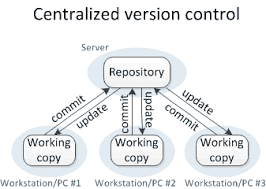
\includegraphics[width=10cm,height=7cm]{Figures/stash.jpg}}
	\caption{Version Control System}
	\label{stash.jpg}
\end{figure}

Version Control System (VCS) adalah perangkat lunak yang membantu 
pengembang perangkat lunak untuk bekerja sama dan menjaga sejarah 
lengkap dari pekerjaan mereka.

\begin{table}[ht]
	\caption{Fungsi VCS}
	\centering
	\begin{tabular}{cccc}
		\hline
		No&Keterangan&\\
		\hline
		.1&Memungkinkan pengembang untuk bekerja secara bersamaan&\\
		.2&Tidak memungkinkan Timpa perubahan masing-masing&\\
		.3&Mempertahankan sejarah setiap versi&\\
		\hline
	\end{tabular}
\end{table}


Berikut ini adalah jenis VCS:

\begin{itemize}
\item sistem kontrol versi terpusat (CVCS).
\item Didistribusikan / Desentralisasi sistem kontrol versi (DVCS).
\end{itemize}
Dalam bab ini, kita akan berkonsentrasi hanya pada sistem kontrol versi 
didistribusikan dan terutama pada Git. Git berada di bawah sistem 
kontrol versi terdistribusi.

\subsection{Distributed Sistem Kontrol Versi}
sistem terpusat kontrol versi (CVCS) menggunakan server pusat untuk 
menyimpan semua file dan memungkinkan kolaborasi tim. Tapi kelemahan 
utama dari CVCS adalah titik tunggal kegagalan, yaitu, kegagalan server 
pusat. Sayangnya, jika server pusat turun selama satu jam, kemudian pada 
jam itu, tidak ada yang bisa berkolaborasi sama sekali. Dan bahkan dalam 
kasus terburuk, jika disk server pusat akan rusak dan cadangan yang 
tepat belum diambil, maka Anda akan kehilangan seluruh sejarah proyek. 
Di sini, sistem terdistribusi kontrol versi (DVCS) datang ke dalam 
gambar.\vspace{14pt}

DVCS klien tidak hanya memeriksa snapshot terbaru dari direktori tetapi 
mereka juga penuh dari repositori tersebut. Jika memutuskan turun, maka 
repositori dari klien dapat disalin kembali ke server untuk 
mengembalikannya. Setiap checkout adalah salinan lengkap dari 
repositori. Git tidak bergantung pada server pusat dan itulah sebabnya 
Anda dapat melakukan banyak operasi ketika Anda sedang offline. Anda 
dapat melakukan perubahan, membuat cabang, lihat log, dan melakukan 
operasi lain ketika Anda sedang offline. Anda memerlukan koneksi 
jaringan hanya untuk mempublikasikan perubahan dan mengambil perubahan 
terbaru.

\subsection{Keuntungan dari Git}\vspace{14pt}

{\textbf{free dan open source}}\vspace{14pt}

Git dirilis di bawah lisensi open source GPL ini. Ini tersedia secara 
bebas melalui internet. Anda dapat menggunakan Git untuk mengelola 
proyek kepatutan tanpa membayar satu sen dolar. Karena merupakan open 
source, Anda dapat men-download kode sumbernya dan juga melakukan 
perubahan sesuai dengan kebutuhan Anda.\vspace{14pt}


{\textbf{Cepat dan kecil}}\vspace{14pt}

Karena sebagian besar operasi dilakukan secara lokal, memberikan manfaat 
yang sangat besar dalam hal kecepatan. Git tidak bergantung pada server 
pusat; itu sebabnya, tidak ada kebutuhan untuk berinteraksi dengan 
server remote untuk setiap operasi. Bagian inti dari Git ditulis dalam 
C, yang menghindari overhead runtime yang terkait dengan bahasa tingkat 
tinggi lainnya. Meskipun Git cermin seluruh repositori, ukuran data di 
sisi client kecil. Ini menggambarkan efisiensi Git di mengompresi dan 
menyimpan data di sisi client.\vspace{14pt}


	{\textbf{backup implisit}}\vspace{14pt}

Kemungkinan kehilangan data sangat jarang ketika ada beberapa salinan 
dari itu. Data hadir di setiap sisi klien cermin repositori, karena itu 
dapat digunakan dalam hal terjadi kecelakaan atau korupsi disk.\vspace{14pt}


{\textbf{Keamanan}}\vspace{14pt}

Git menggunakan fungsi hash kriptografi umum yang disebut fungsi hash 
aman (SHA1), untuk nama dan mengidentifikasi objek dalam database. 
Setiap file dan komit check-dijumlahkan dan diambil oleh checksum-nya 
pada saat checkout. Ini menyiratkan bahwa, tidak mungkin untuk mengubah 
file, tanggal, dan pesan komit dan data lainnya dari database Git tanpa 
mengetahui Git.\vspace{14pt}


	{\textbf{Tidak perlu perangkat keras yang kuat}}\vspace{14pt}

Dalam kasus CVCS, server pusat harus cukup kuat untuk melayani 
permintaan dari seluruh tim. Untuk tim yang lebih kecil, itu tidak 
masalah, tetapi sebagai ukuran tim tumbuh, keterbatasan hardware server 
dapat menjadi hambatan kinerja. Dalam kasus DVCS, pengembang tidak 
berinteraksi dengan server kecuali mereka butuhkan untuk mendorong atau 
menarik perubahan. Semua angkat berat terjadi pada sisi klien, sehingga 
hardware server dapat memang sangat sederhana.\vspace{14pt}


{\textbf{percabangan mudah}\vspace{14pt}

CVCS menggunakan mekanisme copy murah, Jika kita membuat cabang baru, 
itu akan menyalin semua kode ke cabang baru, sehingga memakan waktu dan 
tidak efisien. Juga, penghapusan dan penggabungan cabang di CVCS rumit 
dan memakan waktu. Tapi manajemen cabang dengan Git sangat sederhana. 
Dibutuhkan hanya beberapa detik untuk membuat, menghapus, dan 
menggabungkan cabang.






\chapter{Move Operation}
\section{Move Operation}
\hspace*{0.5in}Seperti namanya, operasi memindahkan direktori atau file dari satu lokasi ke lokasi lain. direktori yang dimodifikasi akan muncul sebagai berikut: \par
\vspace{10pt}
\begin{verbatim}
[tom@CentOS project] $  \$  $ pwd} 

/home/tom/project} 
[tom@CentOS project] $  \$  $ ls} 

{README string string.c} 
[tom@CentOS project] $  \$  $ mkdir src

[tom@CentOS project] $  \$  $ git mv string.c src/} 

[tom@CentOS project] $  \$  $ git status -s

R string.c  $ - $> src/string.c

?? string}
\end{verbatim}

\vspace{10pt}
\hspace*{0.5in} Untuk membuat perubahan ini permanen, harus mendorong struktur direktori yang dimodifikasi ke repositori jauh sehingga pengembang lain dapat melihat ini. \par

\noindent 
[tom@CentOS project] $  \$  $ git commit -m "Modified directory structure" \par
\vspace{12pt}
\noindent 
[master 7d9ea97] Modified directory structure \par
\noindent 
1 files changed, 0 insertions(+), 0 deletions(-) \par
\noindent 
rename string.c => src/string.c (100 $  \%  $) \par
\vspace{12pt}
\noindent 
[tom@CentOS project] $  \$  $ git push origin master \par
\noindent 
Counting objects: 4, done. \par
\noindent 
Compressing objects: 100 $  \%  $ (2/2), done. \par
\noindent 
Writing objects: 100 $  \%  $ (3/3), 320 bytes, done. \par
\noindent 
Total 3 (delta 0), reused 0 (delta 0) \par
\noindent 
To gituser@git.server.com:project.git \par
\noindent 
e86f062..7d9ea97 master  $ - $> master \par

\vspace{12pt}
\hspace*{0.5in} Di gudang lokal Jerry, sebelum operasi penarikan, ia akan menunjukkan struktur direktori lama. \par

\vspace{12pt}
\noindent 
[jerry@CentOS project] $  \$  $ pwd \par
\noindent 
/home/jerry/jerry $  \_  $repo/project \par
\vspace{12pt}
\noindent 
[jerry@CentOS project] $  \$  $ ls \par
\noindent 
README string string.c \par

\vspace{12pt}
\noindent 
 \hspace*{0.5in} Tapi setelah operasi tarik, struktur direktori akan diperbarui. Sekarang, Jerry bisa melihat direktori src dan file yang ada di dalam direktori itu. \par
\noindent 
[jerry@CentOS project] $  \$  $ git pull \par
\noindent 
remote: Counting objects: 4, done. \par
\noindent 
remote: Compressing objects: 100 $  \%  $ (2/2), done. \par
\noindent 
remote: Total 3 (delta 0), reused 0 (delta 0) \par
\noindent 
Unpacking objects: 100 $  \%  $ (3/3), done. \par
\noindent 
From git.server.com:project \par
\noindent 
e86f062..7d9ea97 master  $ - $> origin/master \par
\noindent 
First, rewinding head to replay your work on top of it... \par
\noindent 
Fast-forwarded master to 7d9ea97683da90bcdb87c28ec9b4f64160673c8a. \par
\vspace{12pt}
\noindent 
[jerry@CentOS project] $  \$  $ ls \par
\noindent 
README src string \par
\vspace{12pt}
\noindent 
[jerry@CentOS project] $  \$  $ ls src/ \par
\noindent 
string.c \par

\subsection{Semua Operasi Dilakukan Secara Lokal}
\par
\hspace*{0.5in} Kebanyakan operasi pada Git hanya membutuhkan berkas-berkas dan resource lokal – tidak ada informasi yang dibutuhkan dari komputer lain pada jaringan. Jika terbiasa dengan VCS terpusat dimana kebanyakan operasi memiliki overhead latensi jaringan, aspek Git satu ini akan membuat berpikir bahwa para dewa kecepatan telah memberkati Git dengan kekuatan. Karena memiliki seluruh sejarah dari proyek di lokal disk, dengan kebanyakan operasi yang tampak hampir seketika. \par
\hspace*{0.5in} Sebagai contoh, untuk melihat history dari proyek, Git tidak membutuhkan data histori dari server untuk kemudian menampilkannya untuk, namun secara sedarhana Git membaca historinya langsung dari basisdata lokal proyek tersebut. Ini berarti melihat histori proyek hampir secara instant. Jika ingin membandingkan perubahan pada sebuah berkas antara versi saat ini dengan versi sebulan yang lalu, Git dapat mencari berkas yang sama pada sebulan yang lalu dan melakukan pembandingan perubahan secara lokal, bukan dengan cara meminta remote server melakukannya atau meminta server mengirimkan berkas versi yang lebih lama kemudian membandingkannya secara lokal. \par
\hspace*{0.5in} Hal ini berarti bahwa sangat sedikit yang tidak bisa kerjakan jika sedang offline atau berada diluar VPN. Jika sedang berada dalam pesawat terbang atau sebuah kereta dan ingin melakukan pekerjaan kecil, dapat melakukan commit sampai memperoleh koneksi internet hingga dapat menguploadnya. Jika pulang ke rumah dan VPN client tidak bekerja dengan benar, tetap dapat bekerja. Pada kebanyakan sistem lainnya, melakukan hal ini cukup sulit atau bahkan tidak mungkin sama sekali. Pada Perforce misalnya, tidak dapat berbuat banyak ketika tidak terhubung dengan server; pada Subversion dan CVS,  dapat mengubah berkas, tapi tidak dapat melakukan commit pada basisdata (karena tidak terhubung dengan basisdata). Hal ini mungkin saja bukanlah masalah yang besar, namun akan terkejut dengan perbedaan besar yang disebabkannya. \par

\subsection{Git Memiliki Integritas }
\par
\hspace*{0.5in} Segala sesuatu pada Git akan melalui proses checksum terlebih dahulu sebelum disimpan yang kemudian direferensikan oleh hasil checksum tersebut. Hal ini berarti tidak mungkin melakukan perubahan terhadap berkas manapun tanpa diketahui oleh Git. Fungsionalitas ini dimiliki oleh Git pada level terendahnya dan ini merupakan bagian tak terpisahkan dari filosofi Git. Tidak akan kehilangan informasi atau mendapatkan file yang cacat tanpa diketahui oleh Git. \par
\hspace*{0.5in} Mekanisme checksum yang digunakan oleh Git adalah SHA-1 hash. Ini merupakan sebuah susunan string yang terdiri dari 40 karakter heksadesimal (0 hingga 9 dan a hingga f) dan dihitung berdasarkan isi dari sebuah berkas atau struktur direktori pada Git. sebuah hash SHA-1 berupa seperti berikut: \par
\noindent 
24b9da6552252987aa493b52f8696cd6d3b00373 \par
\vspace{12pt}
\hspace*{0.5in}Nilai seperti ini pada berbagai tempat di Git. Faktanya, Git tidak menyimpan nama berkas pada basisdatanya, melainkan nilai hash dari isi berkas. \par
\hspace*{0.5in} Ketika melakukan operasi pada Git, kebanyakan dari operasi tersebut hanya menambahkan data pada basisdata Git. Seperti pada berbagai VCS, dapat kehilangan atau mengacaukan perubahan yang belum di-commit; namun jika melakukan commit pada Git akan sangat sulit kehilangannya, terutama jika  secara teratur melakukan push basisdata pada repositori lain. \par
\hspace*{0.5in} Hal ini menjadikan Git menyenangkan karena kita dapat berexperimen tanpa kehawatiran untuk mengacaukan proyek. Git memiliki 3 keadaan utama dimana berkas dapat berada: committed, modified dan staged. Committed berarti data telah tersimpan secara aman pada basisdata lokal. Modified berarti telah melakukan perubahan pada berkas namun belum melakukan commit pada basisdata. Staged berarti telah menandai berkas yang telah diubah pada versi yang sedang berlangsung untuk kemudian dilakukan commit. \par
\hspace*{0.5in} Direktori Git adalah dimana Git menyimpan metadata dan database objek untuk projek. Ini adalah bahagian terpenting dari Git, dan inilah yang disalin ketika melakukan kloning sebuah repository dari komputer lain. \par
\noindent 
\hspace*{0.5in} Direktori kerja adalah sebuah checkout tunggal dari satu versi dari projek. Berkas-berkas ini kemudian ditarik keluar dari basisdata yang terkompresi dalam direktori Git dan disimpan pada disk untuk gunakan atau modifikasi. \par
\hspace*{0.5in} Staging area adalah sebuah berkas sederhana, umumnya berada dalam direktori Git, yang menyimpan informasi mengenai apa yang menjadi commit selanjutnya. Ini terkadang disebut sebagai index, tetapi semakin menjadi standard untuk menyebutnya sebagai staging area.Alur kerja dasar Git adalah seperti ini: \par
\noindent 
 \par
\hspace*{0.5in} Jika sebuah versi tertentu dari sebuah berkas telah ada di direktori git dianggap 'committed'. Jika berkas diubah (modified) tetapi sudah ditambahkan ke staging area  maka itu adalah 'staged'. Dan jika berkas telah diubah sejak terakhir dilakukan checked out tetapi belum ditambahkan ke staging area maka itu adalah 'modified'.  \par

\subsection*{13.3 Perintah Untuk Membuat Sebuah Proyek }
\hspace*{0.5in} Membuat direktori baru di repositori Git dengan git init. Melakukan direktori setiap saat, benar-benar lokal. Executive git init dalam direktori, Membuat Git repositori. Sebagai contoh, buat item w3big:  \par
\noindent 
{\fontsize{10pt}{10pt}\selectfont  $  \$  $ mkdir w3big} \par
\noindent 
{\fontsize{10pt}{10pt}\selectfont  $  \$  $ cd w3big/} \par
\noindent 
{\fontsize{10pt}{10pt}\selectfont  $  \$  $ git init} \par
\noindent 
{\fontsize{10pt}{10pt}\selectfont Initialized empty Git repository in /Users/tianqixin/www/w3big/.git/} \par
\noindent 
{\fontsize{10pt}{10pt}\selectfont  $  \#  $ 在 /www/w3big/.git/ 目录初始化空 Git 仓库完毕。} \par
\vspace{14pt}
\hspace*{0.5in} Sekarang dapat melihat subdirektori git yang dihasilkan dalam proyek. Ini adalah repositori Git, dan semua data yang terkait dengan snapshot dari proyek disimpan di sini. \par
\noindent 
{\fontsize{10pt}{10pt}\selectfont ls -a} \par

\vspace{12pt}
\hspace*{0.5in} Gunakan git clone repositori Git untuk salinan lokal, sehingga dapat melihat item atau memodifikasinya. Jika membutuhkan sebuah proyek kerjasama dengan orang lain atau ingin menyalin sebuah proyek, melihat kode, dapat mengkloning proyek. Jalankan:  \par
\noindent 
{\fontsize{10pt}{10pt}\selectfont git clone [url]} \par
\vspace{12pt}
\noindent 
Sebagai contoh, kloning proyek pada Github: \par
\noindent 
{\fontsize{10pt}{10pt}\selectfont  $  \$  $ git clone git@github.com:schacon/simplegit.git} \par
\noindent 
{\fontsize{10pt}{10pt}\selectfont Cloning into 'simplegit'...} \par
\noindent 
{\fontsize{10pt}{10pt}\selectfont remote: Counting objects: 13, done.} \par
\noindent 
{\fontsize{10pt}{10pt}\selectfont remote: Total 13 (delta 0), reused 0 (delta 0), pack-reused 13} \par
\noindent 
{\fontsize{10pt}{10pt}\selectfont Receiving objects: 100 $  \%  $ (13/13), done.} \par
\noindent 
{\fontsize{10pt}{10pt}\selectfont Resolving deltas: 100 $  \%  $ (2/2), done.} \par
\noindent 
{\fontsize{10pt}{10pt}\selectfont Checking connectivity... done.} \par
\vspace{12pt}
\noindent 
\hspace*{0.5in} Setelah kloning selesai di direktori saat ini akan menghasilkan simplegit direktori:  \par
\noindent 
{\fontsize{10pt}{10pt}\selectfont  $  \$  $ Cd simplegit /  $  \$  $ ls README Rakefile lib } \par
\noindent 
operasi akan menyalin semua catatan proyek.  \par
\vspace{12pt}
\noindent 
{\fontsize{10pt}{10pt}\selectfont  $  \$  $ ls -a} \par
\noindent 
{\fontsize{10pt}{10pt}\selectfont git~~~~ README   Rakefile lib} \par
\noindent 
{\fontsize{10pt}{10pt}\selectfont  $  \$  $ cd .git} \par
\noindent 
{\fontsize{10pt}{10pt}\selectfont  $  \$  $ ls} \par
\noindent 
{\fontsize{10pt}{10pt}\selectfont HEAD~~~~~~~~description~info~~~~~   packed-refs} \par
\noindent 
{\fontsize{10pt}{10pt}\selectfont branches~~~~hooks~~~~~~~logs~~~~~   refs} \par
\noindent 
{\fontsize{10pt}{10pt}\selectfont config~~~~~~index~~~~~  objects} \par
\vspace{12pt}
\hspace*{0.5in}Secara default, Git akan mengikuti nama URL yang tersedia item untuk membuat direktori proyek lokalditunjukkan. URL biasanya nama item terakhir / setelah. Jika ingin nama yang berbeda  dapat menambahkan nama yang inginkan setelah perintah. \par

\subsection*{13.4 Snapshot Dasar }
 \par
\hspace*{0.5in} Pekerjaan Git adalah untuk membuat dan menyimpan snapshot dari proyek dan setelah snapshot dan membandingkan. Bab ini akan tentang menciptakan sebuah snapshot dari proyek  dan mengirimkan pengenalan perintah. Git add perintah untuk menambahkan file ke cache, seperti yang tambahkan dua file berikut: \par
\noindent 
{\fontsize{10pt}{10pt}\selectfont  $  \$  $ touch README} \par
\noindent 
{\fontsize{10pt}{10pt}\selectfont  $  \$  $ touch hello.php} \par
\noindent 
{\fontsize{10pt}{10pt}\selectfont  $  \$  $ ls} \par
\noindent 
{\fontsize{10pt}{10pt}\selectfont README hello.php} \par
\noindent 
{\fontsize{10pt}{10pt}\selectfont  $  \$  $ git status -s} \par
\noindent 
{\fontsize{10pt}{10pt}\selectfont ?? README} \par
\noindent 
{\fontsize{10pt}{10pt}\selectfont ?? hello.php} \par
\noindent 
{\fontsize{10pt}{10pt}\selectfont  $  \$  $ } \par
\vspace{12pt}
\noindent 
 \hspace*{0.5in}Perintah git status digunakan untuk melihat status proyek. Selanjutnya jalankan git add perintah untuk menambahkan file: } \par
\noindent 
{\fontsize{10pt}{10pt}\selectfont  $  \$  $ git add README hello.php } \par

\vspace{12pt}
\hspace*{0.5in} Sekarang jalankan git status, dapat melihat dua dokumen tersebut telah ditambahkan untuk pergi : \par
\noindent 
{\fontsize{10pt}{10pt}\selectfont  $  \$  $ git status -s} \par
\noindent 
{\fontsize{10pt}{10pt}\selectfont A~ README} \par
\noindent 
{\fontsize{10pt}{10pt}\selectfont A~ hello.php} \par
\noindent 
{\fontsize{10pt}{10pt}\selectfont  $  \$  $ } \par

\vspace{12pt}
\hspace*{0.5in} Proyek baru, menambahkan semua file yang sama, kita dapat menggunakangit add. Perintah untuk menambahkan semua file dalam proyek saat ini. Sekarang memodifikasi file README:   \par
\noindent 
{\fontsize{10pt}{10pt}\selectfont  $  \$  $ vim README} \par
\noindent 
{\fontsize{10pt}{10pt}\selectfont <pre>} \par
\noindent 
{\fontsize{10pt}{10pt}\selectfont <p>在 README 添加以下内容:<b> $  \#  $ w3big Git 测试</b>,然后保存退出。</p>} \par
\noindent 
{\fontsize{10pt}{10pt}\selectfont <p>再执行一下 git status:</p>} \par
\noindent 
{\fontsize{10pt}{10pt}\selectfont  $  \$  $ git status -s} \par
\noindent 
{\fontsize{10pt}{10pt}\selectfont AM README} \par
\noindent 
{\fontsize{10pt}{10pt}\selectfont A~ hello.php} \par
\vspace{12pt}
\hspace*{0.5in}"AM" status berarti bahwa file tersebut setelah kami menambahkannya ke cache ada perubahan. Setelah perubahan menjalankan git add perintah untuk menambahkannya ke cache: \par
\noindent 
{\fontsize{10pt}{10pt}\selectfont  $  \$  $ git add .} \par
\noindent 
{\fontsize{10pt}{10pt}\selectfont  $  \$  $ git status -s} \par
\noindent 
{\fontsize{10pt}{10pt}\selectfont A~ README} \par
\noindent 
{\fontsize{10pt}{10pt}\selectfont A~ hello.php} \par
\vspace{12pt}
\hspace*{0.5in} Bila ingin perubahan yang terkandung dalam snapshot laporan yang akan datang dalam waktu, harus menjalankan git add. \par
\hspace*{0.5in} Git status untuk melihat setelah komit terakhir jika ada perubahan. Menunjukkan perintah ini ketika ditambahkan -s parameter untuk mendapatkan hasil yang singkat. Jika  tidak menambahkan parameter ini akan keluaran rinci:  \par
\noindent 
~  $  \$  $ git status \par
\noindent 
{\fontsize{10pt}{10pt}\selectfont On branch master} \par
\noindent 
\vspace{10pt}
\noindent 
{\fontsize{10pt}{10pt}\selectfont Initial commit} \par
\noindent 
\vspace{10pt}

\vspace{80pt}
{\fontsize{10pt}{10pt}\selectfont Changes to be committed:} \par
\noindent 
{\fontsize{10pt}{10pt}\selectfont ~ (use "git rm --cached <file>..." to unstage)} \par
\noindent 
\vspace{10pt}
\noindent 
{\fontsize{10pt}{10pt}\selectfont  \hspace*{0.64in} new~file:~  README} \par
\noindent 
{\fontsize{10pt}{10pt}\selectfont  \hspace*{0.64in} new~file:~  hello.php} \par
\vspace{12pt}
\hspace*{0.5in} Status git diff git eksekutif untuk melihat rincian hasil eksekusi. Git perintah diff dan menampilkan cache write telah dimodifikasi tapi belum ditulis ke cache perubahan perbedaan. git diff Ada dua skenario utama.  \par
\noindent 
\begin{itemize}
\item Perubahan tidak cache:diff git  \par
\noindent 
\item Lihatperubahan cache: git diff --cached \par
\noindent 
\item Lihat cache dan uncached semuaperubahan: git diff KEPALA \par
\noindent 
\item Tampilkan ringkasan daripada seluruhdiff: git diff --stat\end{itemize}
 \par
 

\vspace{12pt}
\noindent 
Masukkan berikut dalam file hello.php:  \par
\begin{verbatim}
<?php
echo 'www.w3big.com';
?>
git status -s
A README
AM hello.php
git diff
diff --git a/hello.php b/hello.php
index e69de29..69b5711 100644
--- a/hello.php
+++ b/hello.php
@@ -0,0 +1,3 @@
+<?php
+echo ':www.w3big.com';
+?>
\end{verbatim}

\vspace{10pt}
\hspace*{0.5in}Menampilkan status git pada untuk berubah setelah update atau menulis garis perubahan cache dengan garis dan git diff menunjukkan secara spesifik apa perubahan tersebut.  Selanjutnya melihat git berikutnya diff pelaksanaan --cached hasil:  \par
\noindent 
{\fontsize{10pt}{10pt}\selectfont  $  \$  $ git add hello.php } \par
\noindent 
{\fontsize{10pt}{10pt}\selectfont  $  \$  $ git status -s} \par
\noindent 
{\fontsize{10pt}{10pt}\selectfont A~ README} \par
\noindent 
{\fontsize{10pt}{10pt}\selectfont A~ hello.php} \par
\noindent 
{\fontsize{10pt}{10pt}\selectfont  $  \$  $ git diff --cached} \par
\noindent 
{\fontsize{10pt}{10pt}\selectfont diff --git a/README b/README} \par
\noindent 
{\fontsize{10pt}{10pt}\selectfont new file mode 100644} \par
\noindent 
{\fontsize{10pt}{10pt}\selectfont index 0000000..8f87495} \par
\noindent 
{\fontsize{10pt}{10pt}\selectfont --- /dev/null} \par
\noindent 
{\fontsize{10pt}{10pt}\selectfont +++ b/README} \par
\noindent 
{\fontsize{10pt}{10pt}\selectfont @@ -0,0 +1 @@} \par
\noindent 
{\fontsize{10pt}{10pt}\selectfont + $  \#  $ w3big Git 测试} \par
\noindent 
{\fontsize{10pt}{10pt}\selectfont diff --git a/hello.php b/hello.php} \par
\noindent 
{\fontsize{10pt}{10pt}\selectfont new file mode 100644} \par
\noindent 
{\fontsize{10pt}{10pt}\selectfont index 0000000..69b5711} \par
\noindent 
{\fontsize{10pt}{10pt}\selectfont --- /dev/null} \par
\noindent 
{\fontsize{10pt}{10pt}\selectfont +++ b/hello.php} \par
\noindent 
{\fontsize{10pt}{10pt}\selectfont @@ -0,0 +1,3 @@} \par
\noindent 
{\fontsize{10pt}{10pt}\selectfont +<?php} \par
\noindent 
{\fontsize{10pt}{10pt}\selectfont +echo '本教程:www.w3big.com';} \par
\noindent 
{\fontsize{10pt}{10pt}\selectfont +?>} \par
\vspace{12pt}
\hspace*{0.5in} Gunakan git menambahkan perintah ingin menulis isi dari buffer snapshot, dan mengeksekusi git commit akan menambahkan konten ke gudang penyangga. Git mengirimkan masing-masing nama dan alamat e-mail yang tercatat, sehingga langkah pertama perlu mengkonfigurasi nama pengguna dan alamat e-mail.  \par
\noindent 
{\fontsize{10pt}{10pt}\selectfont  $  \$  $ git config --global user.name 'w3big'} \par
\noindent 
{\fontsize{10pt}{10pt}\selectfont  $  \$  $ git config --global user.email test@w3big.com} \par
\vspace{12pt}
\hspace*{0.5in} Berikutnya menulis caching, dan menyerahkan semua perubahan hello.php tersebut. Dalam contoh pertama menggunakan opsi -m untuk memberikan baris perintah untuk mengirimkan komentar : \par
\noindent 
{\fontsize{10pt}{10pt}\selectfont  $  \$  $ git add hello.php} \par
\noindent 
{\fontsize{10pt}{10pt}\selectfont  $  \$  $ git status -s} \par
\noindent 
{\fontsize{10pt}{10pt}\selectfont A~ README} \par
\noindent 
{\fontsize{10pt}{10pt}\selectfont A~ hello.php} \par
\noindent 
{\fontsize{10pt}{10pt}\selectfont  $  \$  $  $  \$  $ git commit -m '第一次版本提交'} \par
\noindent 
{\fontsize{10pt}{10pt}\selectfont [master (root-commit) d32cf1f] 第一次版本提交} \par
\noindent 
{\fontsize{10pt}{10pt}\selectfont  2 files changed, 4 insertions(+)} \par
\noindent 
{\fontsize{10pt}{10pt}\selectfont  create mode 100644 README} \par
\noindent 
{\fontsize{10pt}{10pt}\selectfont  create mode 100644 hello.php} \par
\noindent 
{\fontsize{10pt}{10pt}\selectfont  } \par

\vspace{12pt}
Sekarang telah mencatat snapshot. Jika di jalankan git status:  \par
\noindent 
{\fontsize{10pt}{10pt}\selectfont  $  \$  $ git status} \par
\noindent 
{\fontsize{10pt}{10pt}\selectfont  $  \#  $ On branch master} \par
\noindent 
{\fontsize{10pt}{10pt}\selectfont nothing to commit (working directory clean)} \par
\vspace{12pt}
\hspace*{0.5in} Output di atas menunjukkan bahwa setelah pengajuan terakhir, tidak membuat perubahan apapu. Jika tidak menetapkan opsi -m, Git mencoba untuk membuka editor untuk mengisi informasi yang disampaikan. Git jika tidak dapat menemukan informasi yang relevan dalam konfigurasi, default akan membuka vim. Layar akan terlihat seperti ini:  \par
\noindent 
{\fontsize{10pt}{10pt}\selectfont  $  \#  $ Please enter the commit message for your changes. Lines starting} \par
\noindent 
{\fontsize{10pt}{10pt}\selectfont  $  \#  $ with ' $  \#  $' will be ignored, and an empty message aborts the commit.} \par
\noindent 
{\fontsize{10pt}{10pt}\selectfont  $  \#  $ On branch master} \par
\noindent 
{\fontsize{10pt}{10pt}\selectfont  $  \#  $ Changes to be committed:} \par
\noindent 
{\fontsize{10pt}{10pt}\selectfont  $  \#  $~~ (use "git reset HEAD <file>..." to unstage)} \par
\noindent 
{\fontsize{10pt}{10pt}\selectfont  $  \#  $} \par
\noindent 
{\fontsize{10pt}{10pt}\selectfont  $  \#  $~modified:~  hello.php} \par
\noindent 
{\fontsize{10pt}{10pt}\selectfont  $  \#  $} \par
\noindent 
{\fontsize{10pt}{10pt}\selectfont  $  \sim  $} \par
\noindent 
{\fontsize{10pt}{10pt}\selectfont  $  \sim  $} \par
\noindent 
{\fontsize{10pt}{10pt}\selectfont ".git/COMMIT $  \_  $EDITMSG" 9L, 257C} \par
\vspace{12pt}
\hspace*{0.5in} Jika berpikir git add disampaikan proses cache yang terlalu rumit, Git juga memungkinkan untuk menggunakan opsi -a untuk melewatkan langkah ini. format perintah adalah sebagai berikut: \par
\noindent 
{\fontsize{10pt}{10pt}\selectfont git commit -a} \par
\vspace{12pt}
\noindent 
Memodifikasi file hello.php sebagai berikut:  \par
\noindent 
{\fontsize{10pt}{10pt}\selectfont <?php} \par
\noindent 
{\fontsize{10pt}{10pt}\selectfont echo '本教程:www.w3big.com';} \par
\noindent 
{\fontsize{10pt}{10pt}\selectfont echo '本教程:www.w3big.com';} \par
\noindent 
{\fontsize{10pt}{10pt}\selectfont ?>} \par
\vspace{10pt}
\noindent 
Kemudian jalankan perintah berikut:  \par
\noindent 
{\fontsize{10pt}{10pt}\selectfont git commit -am '修改 hello.php 文件'} \par
\noindent 
{\fontsize{10pt}{10pt}\selectfont [master 71ee2cb] 修改 hello.php 文件} \par
\noindent 
{\fontsize{10pt}{10pt}\selectfont  1 file changed, 1 insertion(+)} \par
\vspace{10pt}
\hspace*{0.5in} Git reset perintah HEAD untuk menghapus konten cache.  Mari mengubah file berkas README, sebagai berikut:  \par
\noindent 
{\fontsize{10pt}{10pt}\selectfont  $  \#  $ w3big Git 测试} \par
\noindent 
{\fontsize{10pt}{10pt}\selectfont  $  \#  $ 本教程 } \par
\vspace{12pt}
\noindent 
File hello.php diubah sebagai berikut:  \par
\noindent 
{\fontsize{10pt}{10pt}\selectfont <?php} \par
\noindent 
{\fontsize{10pt}{10pt}\selectfont echo '本教程:www.w3big.com';} \par
\noindent 
{\fontsize{10pt}{10pt}\selectfont echo '本教程:www.w3big.com';} \par
\noindent 
{\fontsize{10pt}{10pt}\selectfont echo '本教程:www.w3big.com';} \par
\noindent 
{\fontsize{10pt}{10pt}\selectfont ?>} \par
\vspace{10pt}
\hspace*{0.5in} Sekarang setelah dua file diubah disampaikan ke zona penyangga, sekarang ingin membatalkan salah satu dari cache, sebagai berikut: \par
\noindent 
{\fontsize{10pt}{10pt}\selectfont  $  \$  $ git status -s} \par
\noindent 
{\fontsize{10pt}{10pt}\selectfont  M README} \par
\noindent 
{\fontsize{10pt}{10pt}\selectfont  M hello.php} \par
\noindent 
{\fontsize{10pt}{10pt}\selectfont  $  \$  $ git add .} \par
\noindent 
{\fontsize{10pt}{10pt}\selectfont  $  \$  $ git status -s} \par
\noindent 
{\fontsize{10pt}{10pt}\selectfont M~ README} \par
\noindent 
{\fontsize{10pt}{10pt}\selectfont M~ hello.pp} \par
\noindent 
{\fontsize{10pt}{10pt}\selectfont  $  \$  $ git reset HEAD -- hello.php } \par
\noindent 
{\fontsize{10pt}{10pt}\selectfont Unstaged changes after reset:} \par
\noindent 
{\fontsize{10pt}{10pt}\selectfont M \hspace*{0.64in} hello.php} \par
\noindent 
{\fontsize{10pt}{10pt}\selectfont  $  \$  $ git status -s} \par
\noindent 
{\fontsize{10pt}{10pt}\selectfont M~ README} \par
\noindent 
{\fontsize{10pt}{10pt}\selectfont  M hello.php} \par
\vspace{12pt}
\hspace*{0.5in} Sekarang menjalankan git commit, perubahan hanya akan diserahkan berkas README, tapi hello.php tidak.  \par
\noindent 
{\fontsize{10pt}{10pt}\selectfont  $  \$  $ git commit -m '修改'} \par
\noindent 
{\fontsize{10pt}{10pt}\selectfont [master f50cfda] 修改} \par
\noindent 
{\fontsize{10pt}{10pt}\selectfont  1 file changed, 1 insertion(+)} \par
\noindent 
{\fontsize{10pt}{10pt}\selectfont  $  \$  $ git status -s} \par
\noindent 
{\fontsize{10pt}{10pt}\selectfont  M hello.php} \par
\vspace{12pt}
\hspace*{0.5in} Melihat file perubahan hello.php dan untuk pengajuan. Maka dapat menggunakan perintah berikut untuk memodifikasi hello.php menyerahkan:  \par
\noindent 
{\fontsize{10pt}{10pt}\selectfont  $  \$  $ git commit -am '修改 hello.php 文件'} \par
\noindent 
{\fontsize{10pt}{10pt}\selectfont [master 760f74d] 修改 hello.php 文件} \par
\noindent 
{\fontsize{10pt}{10pt}\selectfont  1 file changed, 1 insertion(+)} \par
\noindent 
{\fontsize{10pt}{10pt}\selectfont  $  \$  $ git status} \par
\noindent 
{\fontsize{10pt}{10pt}\selectfont On branch master} \par
\noindent 
{\fontsize{10pt}{10pt}\selectfont nothing to commit, working directory clean} \par
\vspace{10pt}
\hspace*{0.5in} Singkatnya, melakukan git reset HEAD untuk membatalkan sebelum git add untuk menambahkan, tetapi tidak ingin untuk memasukkan dalam cache snapshot di commit selanjutnya. \par
\hspace*{0.5in} Entri rm git akan dihapus dari cache. ulang kepala git ini membatalkan entri cache yang berbeda. "Batal Cache", yang berarti bahwa pemulihan akan membuat perubahan ke cache.  Secara default, git file rm akan dihapus dari file cache dan hard drive  (direktori kerja). Jika ingin menyimpan file dalam direktori kerja, dapat menggunakangit rm --cached: Seperti kita menghapus hello.php file:  \par
\noindent 
{\fontsize{10pt}{10pt}\selectfont  $  \$  $ git rm hello.php } \par
\noindent 
{\fontsize{10pt}{10pt}\selectfont rm 'hello.php'} \par
\noindent 
{\fontsize{10pt}{10pt}\selectfont  $  \$  $ ls} \par
\noindent 
{\fontsize{10pt}{10pt}\selectfont README} \par

\vspace{50pt}
Tidak menghapus file dari ruang kerja:  \par
\noindent 
{\fontsize{10pt}{10pt}\selectfont  $  \$  $ git rm --cached README } \par
\noindent 
{\fontsize{10pt}{10pt}\selectfont rm 'README'} \par
\noindent 
{\fontsize{10pt}{10pt}\selectfont  $  \$  $ ls} \par
\noindent
{\fontsize{10pt}{10pt}\selectfont README} \par

\vspace{10pt}
\hspace*{0.5in} Git perintah mv untuk melakukan semua hal yanggit rm perintah operasi --cached,mengubah nama file pada disk, dan kemudian jalankan git add untuk menambahkan file baru ke cache.  README pertama kita hapus hanya menambahkan kembali:  \par
\noindent 
{\fontsize{10pt}{10pt}\selectfont  $  \$  $ git add README } \par
\vspace{12pt}
\noindent 
Kemudian nama yang sama yaitu:  \par
\noindent 
{\fontsize{10pt}{10pt}\selectfont  $  \$  $~git mv README  README.md} \par
\noindent 
{\fontsize{10pt}{10pt}\selectfont  $  \$  $ ls} \par
\noindent 
{\fontsize{10pt}{10pt}\selectfont README.md} 

\section{Mendapatkan File untuk Pindah}
\hspace*{0.5in} Buat salinan repositori A sehingga bisa memindahkannya tanpa terlalu mengkhawatirkan kesalahan. Sebaiknya hapus tautan ke repositori asli agar tidak sengaja membuat perubahan jarak jauh (baris 3). Ini berjalan melalui file, menghapus apapun yang tidak ada dalam direktori 1. Hasilnya adalah isi direktori 1 dipindahkan ke basis repositori A. Mengimpor file-file ini ke dalam repositori B di dalam direktori, jadi memindahkan semua menjadi satu sekarang (baris 5/6). Komit perubahan dan menggabungkan file-file ini ke dalam repositori yang baru \ref{PerpindahanFile} :
\begin{figure}[ht]
	\centerline{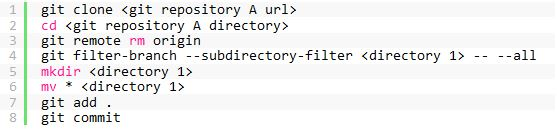
\includegraphics[width=0.50\textwidth]{Figures/PerpindahanFile}}
	\caption{PerpindahanFile}
	\label{PerpindahanFile}
\end{figure}

\chapter{Rename Operation}
Sampai sekarang, baik Tom dan Jerry menggunakan perintah manual untuk menyusun proyek mereka. Sekarang, Jerry memutuskan untuk membuat Makefile untuk proyek mereka dan juga memberi nama yang tepat untuk file "string.c". \par
\noindent 
{\fontsize{10pt}{10pt}\selectfont [jerry@CentOS project] $  \$  $ pwd} \par
\noindent 
{\fontsize{10pt}{10pt}\selectfont /home/jerry/jerry $  \_  $repo/project} \par
\noindent 
\vspace{10pt}
\noindent 
{\fontsize{10pt}{10pt}\selectfont [jerry@CentOS project] $  \$  $ ls} \par
\noindent 
{\fontsize{10pt}{10pt}\selectfont README src} \par
\noindent 
\vspace{10pt}
\noindent 
{\fontsize{10pt}{10pt}\selectfont [jerry@CentOS project] $  \$  $ cd src/} \par
\noindent 
\vspace{10pt}
\noindent 
{\fontsize{10pt}{10pt}\selectfont [jerry@CentOS src] $  \$  $ git add Makefile} \par
\noindent 
\vspace{10pt}
\noindent 
{\fontsize{10pt}{10pt}\selectfont [jerry@CentOS src] $  \$  $ git mv string.c string $  \_  $operations.c} \par
\noindent 
\vspace{10pt}
\noindent 
{\fontsize{10pt}{10pt}\selectfont [jerry@CentOS src] $  \$  $ git status -s} \par
\noindent 
{\fontsize{10pt}{10pt}\selectfont A Makefile} \par
\noindent 
{\fontsize{10pt}{10pt}\selectfont R string.c  $ - $> string $  \_  $operations.c} \par
\vspace{12pt}
Git menunjukkan R sebelum nama file untuk menunjukkan bahwa file telah diganti namanya. \par
Untuk komit operasi, Jerry menggunakan - bendera, yang membuat git komit secara otomatis mendeteksi file yang dimodifikasi. \par
\noindent 
[jerry@CentOS src] $  \$  $ git commit -a -m 'Added Makefile and renamed strings.c to \par
\noindent 
string $  \_  $operations.c ' \par
\vspace{12pt}
\noindent 
[master 94f7b26] Added Makefile and renamed strings.c to string $  \_  $operations.c \par
\noindent 
1 files changed, 0 insertions(+), 0 deletions(-) \par
\noindent 
create mode 100644 src/Makefile \par
\noindent 
rename src/ $  \{  $string.c => string $  \_  $operations.c $  \}  $ (100 $  \%  $) \par
\vspace{12pt}
\noindent 
Setelah komit, dia mendorong perubahannya ke repositori. \par
\noindent 
[jerry@CentOS src] $  \$  $ git push origin master \par
\vspace{12pt}
\noindent 
Perintah di atas akan menghasilkan hasil sebagai berikut: \par
\noindent 
Counting objects: 6, done. \par
\noindent 
Compressing objects: 100 $  \%  $ (3/3), done. \par
\noindent 
Writing objects: 100 $  \%  $ (4/4), 396 bytes, done. \par
\noindent 
Total 4 (delta 0), reused 0 (delta 0) \par
\noindent 
To gituser@git.server.com:project.git \par
\noindent 
7d9ea97..94f7b26 master  $ - $> master \par
\vspace{12pt}
Sekarang, pengembang lain dapat melihat modifikasi ini dengan memperbarui repositori lokal mereka. \par
Kegunaan utama dari sistem kontrol versi ialah sebagai alat untuk manajemen kode program. Terdapat dua kegunaan utama dari sistem ini, yaitu: \par
\noindent 
Menggabungkan perubahan-perubahan kode dari versi lama (misal: untuk mengembalikan fitur yang telah dihapus) ataupun menggabungkan perubahan dari orang lain (misal: menggabungkan fitur yang dikembangkan oleh anggota tim lain).
 \par
\vspace{12pt}
\noindent 
\textbf{14.1 Intalasi Git} \par
git berjalan pada semua sistem operasi populer (Mac, Windows, Linux). Jika menggunakan Windows atau Mac, masuk ke situs utama git pada 
 lalu lakukan download dan instalasi software tersebut. Pengguna Linux dapat melakukan instalasi melalui repositori distribusi yang dilakukan, melalui perintah sejenis: \par
\noindent 
{\fontsize{10pt}{10pt}\selectfont yum install git} \par
\vspace{12pt}
\noindent 
pada repositori berbasis RPM, atau perintah \par
\noindent 
{\fontsize{10pt}{10pt}\selectfont apt-get install git} \par
\vspace{12pt}
Untuk repositori berbasis deb. Kembali lagi, perintah hanya diberikan untuk distribusi paling populer (Debian / Ubuntu dan RedHat / Fedora), karena keterbatasan ruang. Jika menggunakan distrusi lain (seperti Gentoo atau Arch, maka diasumsikan telah mengetahui cara instalasi git atau perangkat lunak lain pada umumnya). \par
Khusus untuk sistem operasi Windows, pastikan instalasi anda diambil dari 
, karena pada paket yang tersedia di website tersebut telah diikutkan juga OpenSSH, yang akan sangat berguna jika ingin berkolaborasi dengan programmer lain. Perintah git juga harus memberikan respon yang benar: \par
\noindent 
{\fontsize{10pt}{10pt}\selectfont bert@LYNNSLENIA  $  \sim  $} \par
\noindent 
{\fontsize{10pt}{10pt}\selectfont  $  \$  $ git} \par
\noindent 
{\fontsize{10pt}{10pt}\selectfont usage: git [--version] [--exec-path[=<path>]] [--html-path] [--man-path] [--info-path]} \par
\noindent 
{\fontsize{10pt}{10pt}\selectfont ~~~~~~~~~~ [-p $  \vert  $--paginate $  \vert  $--no-pager] [--no-replace-objects] [--bare]} \par
\noindent 
{\fontsize{10pt}{10pt}\selectfont ~~~~~~~~~~ [--git-dir=<path>] [--work-tree=<path>] [--namespace=<name>]} \par
\noindent 
{\fontsize{10pt}{10pt}\selectfont ~~~~~~~~~~ [-c name=value] [--help]} \par
\noindent 
{\fontsize{10pt}{10pt}\selectfont ~~~~~~~~~~ <command> [<args>]} \par
\noindent 
{\fontsize{10pt}{10pt}\selectfont The most commonly used git commands are:} \par
\noindent 
{\fontsize{10pt}{10pt}\selectfont ~~~add~~~~~~  Add file contents to the index} \par
\noindent 
{\fontsize{10pt}{10pt}\selectfont ~~~bisect~~~  Find by binary search the change that introduced a bug} \par
\noindent 
{\fontsize{10pt}{10pt}\selectfont ~~~branch~~~  List, create, or delete branches} \par
\noindent 
{\fontsize{10pt}{10pt}\selectfont ~~~checkout~  Checkout a branch or paths to the working tree} \par
\noindent 
{\fontsize{10pt}{10pt}\selectfont ~~~clone~~~~  Clone a repository into a new directory} \par
\noindent 
{\fontsize{10pt}{10pt}\selectfont ~~~commit~~~  Record changes to the repository} \par
\noindent 
{\fontsize{10pt}{10pt}\selectfont ~diff~~~~~  Show changes between commits, commit and working tree, etc} \par
\noindent 
{\fontsize{10pt}{10pt}\selectfont ~~~fetch~~~~  Download objects and refs from another repository} \par
\noindent 
{\fontsize{10pt}{10pt}\selectfont ~~~grep~~~~~  Print lines matching a pattern} \par
\noindent 
{\fontsize{10pt}{10pt}\selectfont ~~~init~~~~~  Create an empty git repository or reinitialize an existing one} \par
\noindent 
{\fontsize{10pt}{10pt}\selectfont ~~~log~~~~~~  Show commit logs} \par
\noindent 
{\fontsize{10pt}{10pt}\selectfont ~~~merge~~~~  Join two or more development histories together} \par
\noindent 
{\fontsize{10pt}{10pt}\selectfont ~~~mv~~~~~~~  Move or rename a file, a directory, or a symlink} \par
\noindent 
{\fontsize{10pt}{10pt}\selectfont ~~~pull~~~~~  Fetch from and merge with another repository or a local branch} \par
\noindent 
{\fontsize{10pt}{10pt}\selectfont ~~~push~~~~~  Update remote refs along with associated objects} \par
\noindent 
{\fontsize{10pt}{10pt}\selectfont ~~~rebase~~~  Forward-port local commits to the updated upstream head} \par
\noindent 
{\fontsize{10pt}{10pt}\selectfont ~~~reset~~~~  Reset current HEAD to the specified state} \par
\noindent 
{\fontsize{10pt}{10pt}\selectfont ~~~rm~~~~~~~  Remove files from the working tree and from the index} \par
\noindent 
{\fontsize{10pt}{10pt}\selectfont ~~~show~~~~~  Show various types of objects} \par
\noindent 
{\fontsize{10pt}{10pt}\selectfont ~~~status~~~  Show the working tree status} \par
\noindent 
{\fontsize{10pt}{10pt}\selectfont ~~~tag~~~~~~  Create, list, delete or verify a tag object signed with GPG} \par
\noindent 
\vspace{10pt}
\noindent 
{\fontsize{10pt}{10pt}\selectfont See 'git help <command>' for more information on a specific command.} \par
\noindent 
{\fontsize{10pt}{10pt}\selectfont bert@LYNNSLENIA  $  \sim  $} \par
\noindent 
{\fontsize{10pt}{10pt}\selectfont  $  \$  $} \par
\vspace{12pt}
\noindent 
\textbf{14.2 Inisiasi} \par
Untuk dapat menggunakan sistem kontrol versi, terlebih dahulu kita harus mempersiapkan repositori. Sebuah repositori menyimpan seluruh versi dari kode program kita. Tidak usah takut, karena repositori tidak akan memakan banyak ruang \emph{hard disk}, karena penyimpanan tidak dilakukan terhadap keseluruhan file. Repositori hanya akan menyimpan \emph{perubahan} yang terjadi pada kode kita dari satu versi ke versi lainnya. Bahasa kerennya, repositori hanya menyimpan delta dari kode pada setiap versinya. \par
Pada (di saat kontrol versi yang populer adalah cvs dan programmer pada umumnya berjanggut putih), membangun repositori kode baru adalah hal yang sangat sulit dilakukan. Harus memiliki sebuah \emph{server} khusus yang dapat diakses oleh seluruh anggota tim. Jika server tidak dapat diakses karena jaringan rusak atau internet putus, maka tidak dapat melakukan kontrol versi (dan harus kembali ke metode direktori, atau tidak bekerja). \par
git merupakan sistem kontrol versi terdistribusi, yang berarti git dapat dijalankan tanpa perlu adanya repositori terpusat. Yang diperlukan untuk membuat repositori ialah mengetikkan perintah tertentu di direktori utama. Mulai membuat repositori baru.: \par
\noindent 
{\fontsize{10pt}{10pt}\selectfont bert@LYNNSLENIA  $  \sim  $} \par
\noindent 
{\fontsize{10pt}{10pt}\selectfont  $  \$  $ cd Desktop/projects/git-tutor/} \par
\noindent 
{\fontsize{10pt}{10pt}\selectfont bert@LYNNSLENIA  $  \sim  $/Desktop/projects/git-tutor} \par
\noindent 
{\fontsize{10pt}{10pt}\selectfont  $  \$  $ ls} \par
\noindent 
{\fontsize{10pt}{10pt}\selectfont bert@LYNNSLENIA  $  \sim  $/Desktop/projects/git-tutor} \par
\noindent 
{\fontsize{10pt}{10pt}\selectfont  $  \$  $} \par
\noindent 
\vspace{10pt}
Menambahkan kode baru ke dalam direktori ini. Buat sebuah file baru yang bernama cerita.txt di dalam direktori tersebut: \par
\noindent 
{\fontsize{10pt}{10pt}\selectfont bert@LYNNSLENIA  $  \sim  $/Desktop/projects/git-tutor} \par
\noindent 
{\fontsize{10pt}{10pt}\selectfont  $  \$  $ echo "ini adalah sebuah cerita" > cerita.txt} \par
\noindent 
\vspace{10pt}
\noindent 
{\fontsize{10pt}{10pt}\selectfont bert@LYNNSLENIA  $  \sim  $/Desktop/projects/git-tutor} \par
\noindent 
{\fontsize{10pt}{10pt}\selectfont  $  \$  $ ls} \par
\noindent 
{\fontsize{10pt}{10pt}\selectfont cerita.txt} \par
\vspace{12pt}
\noindent 
kemudian masukkan perintah git init untuk melakukan inisialisasi repositori: \par
\noindent 
{\fontsize{10pt}{10pt}\selectfont bert@LYNNSLENIA  $  \sim  $/Desktop/projects/git-tutor} \par
\noindent 
{\fontsize{10pt}{10pt}\selectfont  $  \$  $ git init} \par
\noindent 
{\fontsize{10pt}{10pt}\selectfont Initialized empty Git repository in c:/Users/bert/Desktop/projects/git-tutor/.git/} \par
\vspace{12pt}
Setelah melakukan inisialisasi, git secara otomatis akan membuat direktori .git pada repositori  (lihat potongan kode di bawah). Direktori tersebut merupakan direktori yang digunakan oleh git untuk menyimpan basis data delta kode, dan berbagai metadata lainnya. Mengubah direktori tersebut dapat menyebabkan hilangnya seluruh \emph{history} dari kode. \par
\noindent 
{\fontsize{10pt}{10pt}\selectfont bert@LYNNSLENIA  $  \sim  $/Desktop/projects/git-tutor (master)} \par
\noindent 
{\fontsize{10pt}{10pt}\selectfont  $  \$  $ ls -a} \par
\noindent 
{\fontsize{10pt}{10pt}\selectfont .~~..~ .git  cerita.txt} \par
\noindent 
\vspace{10pt}
\noindent 
\textbf{14.3 }\textbf{Penambahan File ke Repository} \par
\noindent 
 \hspace*{0.64in} Penyimpanan sejarah dapat dimulai dari saat pertama: kapan file tersebut dibuat dan ditambahkan ke dalam repositori. Untuk menambahkan file ke dalam repositori, gunakan perintah git add: \par
{\fontsize{10pt}{10pt}\selectfont bert@LYNNSLENIA  $  \sim  $/Desktop/projects/git-tutor (master)} \par
{\fontsize{10pt}{10pt}\selectfont  $  \$  $ git add .} \par
{\fontsize{10pt}{10pt}\selectfont warning: LF will be replaced by CRLF in cerita.txt.} \par
{\fontsize{10pt}{10pt}\selectfont The file will have its original line endings in your working directory.} \par
\noindent 
\vspace{12pt}
\noindent 
Secara sederhana, sintaks dari perintah git add adalah sebagai berikut: \par
{\fontsize{10pt}{10pt}\selectfont git add [nama file atau pola]} \par
\noindent 
\vspace{12pt}
\noindent 
 \hspace*{0.64in} Memasukkan nama file dalam perintah git add pada dasarnya akan memerintahkan git untuk menambahkan \textbf{semua} file baru dalam repositori. Jika hanya ingin menambahkan satu file (misalkan ada file yang belum yakin akan ditambahkan ke repositori), nama file spesifik dapat dimasukkan: \par
{\fontsize{10pt}{10pt}\selectfont git add cerita.txt} \par
\noindent 
\vspace{12pt}
Setelah menambahkan file ke dalam repositori, harus melakukan \emph{commit}. Perintah \emph{commit} memberitahukan kepada git untuk menyimpan sejarah dari file yang telah ditambahkan. Pada git, penambahan, perubahan, ataupun penghapusan sebuah file baru akan tercatat jika perntah \emph{commit} telah dijalankan. Mari lakukan \emph{commit} dengan menjalankan perintah git commit: \par
{\fontsize{10pt}{10pt}\selectfont bert@LYNNSLENIA  $  \sim  $/Desktop/projects/git-tutor (master)} \par
{\fontsize{10pt}{10pt}\selectfont  $  \$  $ git commit} \par
\noindent 
\vspace{12pt}
\noindent 
 \hspace*{0.64in} Jika langkah di atas diikuti dengan benar, maka kembali ke {\fontsize{11pt}{11pt}\selectfont git bash, dengan pesan berikut:} \par
{\fontsize{10pt}{10pt}\selectfont bert@LYNNSLENIA  $  \sim  $/Desktop/projects/git-tutor (master)} \par
{\fontsize{10pt}{10pt}\selectfont  $  \$  $ git commit} \par
{\fontsize{10pt}{10pt}\selectfont [master (root-commit) 1d4cdc9] Inisialisasi repo. Penambahan cerita.txt.} \par
{\fontsize{10pt}{10pt}\selectfont warning: LF will be replaced by CRLF in cerita.txt.} \par
{\fontsize{10pt}{10pt}\selectfont The file will have its original line endings in your working directory.} \par
{\fontsize{10pt}{10pt}\selectfont  1 file changed, 1 insertion(+)} \par
{\fontsize{10pt}{10pt}\selectfont  create mode 100644 cerita.txt} \par
\noindent 
\vspace{12pt}
\noindent 
\textbf{14.4}\textbf{ Mengubah Isi File} \par
Kegunaan utama kontrol versi (yang tercermin dari namanya) ialah melakukan manajemen perubahan secara otomatis untuk kita. dan kemudian jalankan perintah git commit lagi: \par
{\fontsize{10pt}{10pt}\selectfont bert@LYNNSLENIA  $  \sim  $/Desktop/projects/git-tutor (master)} \par
{\fontsize{10pt}{10pt}\selectfont  $  \$  $ git commit} \par
{\fontsize{10pt}{10pt}\selectfont  $  \#  $ On branch master} \par
{\fontsize{10pt}{10pt}\selectfont  $  \#  $ Changes not staged for commit:} \par
{\fontsize{10pt}{10pt}\selectfont  $  \#  $~~ (use "git add <file>..." to update what will be committed)} \par
{\fontsize{10pt}{10pt}\selectfont  $  \#  $~~ (use "git checkout -- <file>..." to discard changes in working directory)} \par
{\fontsize{10pt}{10pt}\selectfont  $  \#  $} \par
{\fontsize{10pt}{10pt}\selectfont  $  \#  $~~~~~~~modified:~  cerita.txt} \par
{\fontsize{10pt}{10pt}\selectfont  $  \#  $} \par
{\fontsize{10pt}{10pt}\selectfont no changes added to commit (use "git add" and/or "git commit -a")} \par
\vspace{12pt}
Perhatikan bahwa git secara otomatis mengetahui file mana saja yang berubah, tetapi tidak melakukan pencatatan perubahan tersebut. Untuk memerintahkan git mencatat perubahan tersebut, gunakan perintah git commit -a: \par
{\fontsize{10pt}{10pt}\selectfont bert@LYNNSLENIA  $  \sim  $/Desktop/projects/git-tutor (master)} \par
{\fontsize{10pt}{10pt}\selectfont  $  \$  $ git commit -a} \par
{\fontsize{10pt}{10pt}\selectfont [master 61c4707] Kapitalisasi dan melengkapi kalimat.} \par
{\fontsize{10pt}{10pt}\selectfont  1 file changed, 1 insertion(+), 1 deletion(-)} \par
\vspace{12pt}
Selain melakukan perubahan, tentunya terkadang kita ingin mengetahui perubahan-perubahan apa saja yang terjadi selama pengembangan. Untuk melihat daftar perubahan yang telah dilakukan, kita dapat menggunakan perintah git log: \par
\noindent 
{\fontsize{10pt}{10pt}\selectfont bert@LYNNSLENIA  $  \sim  $/Desktop/projects/git-tutor (master)} \par
\noindent 
{\fontsize{10pt}{10pt}\selectfont  $  \$  $ git log} \par
\noindent 
{\fontsize{10pt}{10pt}\selectfont commit 61c47074ee583dbdd16fa9568019e80d864fb403} \par
\noindent 
{\fontsize{10pt}{10pt}\selectfont Author: Alex Xandra Albert Sim <bertzzie@gmail.com>} \par
\noindent 
{\fontsize{10pt}{10pt}\selectfont Date:~~ Sun Dec 23 16:36:46 2012 +0700} \par
\noindent 
\vspace{10pt}
\noindent 
{\fontsize{10pt}{10pt}\selectfont ~~~ Kapitalisasi dan melengkapi kalimat.} \par
\noindent 
\vspace{10pt}
\noindent 
{\fontsize{10pt}{10pt}\selectfont commit 1d4cdc9350570230d352ef19aededf06769b0698} \par
\noindent 
{\fontsize{10pt}{10pt}\selectfont Author: Alex Xandra Albert Sim <bertzzie@gmail.com>} \par
\noindent 
{\fontsize{10pt}{10pt}\selectfont Date:~~ Sun Dec 23 16:10:33 2012 +0700} \par
\noindent 
\vspace{10pt}
\noindent 
{\fontsize{10pt}{10pt}\selectfont ~~~ Inisialisasi repo. Penambahan cerita.txt.} \par
\vspace{12pt}
\noindent 
Mari jalankan perintah git log sekali lagi, untuk melihat hasil pekerjaan kita sejauh ini: \par
\noindent 
{\fontsize{10pt}{10pt}\selectfont bert@LYNNSLENIA  $  \sim  $/Desktop/projects/git-tutor (master)} \par
\noindent 
{\fontsize{10pt}{10pt}\selectfont  $  \$  $ git log} \par
\noindent 
{\fontsize{10pt}{10pt}\selectfont commit 28dabb1c54a086cce567ecb890b10339416bcbfa} \par
\noindent 
{\fontsize{10pt}{10pt}\selectfont Author: Alex Xandra Albert Sim <bertzzie@gmail.com>} \par
\noindent 
{\fontsize{10pt}{10pt}\selectfont Date:~~ Sun Dec 23 16:49:21 2012 +0700} \par
\noindent 
\vspace{10pt}
\noindent 
{\fontsize{10pt}{10pt}\selectfont ~~~ Penambahan misteri terbesar di dunia.} \par
\noindent 
\vspace{10pt}
\noindent 
{\fontsize{10pt}{10pt}\selectfont commit 61c47074ee583dbdd16fa9568019e80d864fb403} \par
\noindent 
{\fontsize{10pt}{10pt}\selectfont Author: Alex Xandra Albert Sim <bertzzie@gmail.com>} \par
\noindent 
{\fontsize{10pt}{10pt}\selectfont Date:~~ Sun Dec 23 16:36:46 2012 +0700} \par
\noindent 
\vspace{10pt}
\noindent 
{\fontsize{10pt}{10pt}\selectfont ~~~ Kapitalisasi dan melengkapi kalimat.} \par
\noindent 
\vspace{10pt}
\noindent 
{\fontsize{10pt}{10pt}\selectfont commit 1d4cdc9350570230d352ef19aededf06769b0698} \par
\noindent 
{\fontsize{10pt}{10pt}\selectfont Author: Alex Xandra Albert Sim <bertzzie@gmail.com>} \par
\noindent 
{\fontsize{10pt}{10pt}\selectfont Date:~~ Sun Dec 23 16:10:33 2012 +0700} \par
\noindent 
\vspace{10pt}
\noindent 
{\fontsize{10pt}{10pt}\selectfont ~~~ Inisialisasi repo. Penambahan cerita.txt.} \par
\vspace{12pt}
git memungkinkan kita untuk mengembalikan kode ke dalam keadaan sebelumnya, yaitu \emph{commit} terakhir. Melakukan pengembalian kode ini dengan menggunakan perintah git checkout seperti berikut: \par
\noindent 
bert@LYNNSLENIA  $  \sim  $/Desktop/projects/git-tutor (master) \par
\noindent 
 $  \$  $ git checkout HEAD -- cerita.txt \par
\noindent 
bert@LYNNSLENIA  $  \sim  $/Desktop/projects/git-tutor (master) \par
\noindent 
 $  \$  $ ls \par
\noindent 
cerita.txt \par
\noindent 
bert@LYNNSLENIA  $  \sim  $/Desktop/projects/git-tutor (master) \par
\noindent 
 $  \$  $ cat cerita.txt \par
\noindent 
Ini adalah sebuah cerita tentang seekor kera yang terkurung dan terpenjara dalam goa. \par
\noindent 
Kera ini bernama Sun Go Kong. Dari manakah Sun Go Kong berasal? \par
\noindent 
bert@LYNNSLENIA  $  \sim  $/Desktop/projects/git-tutor (master) \par
\vspace{12pt}
Parameter HEAD pada perintah yang kita jalankan merupakan parameter untuk memberitahukan git checkout bahwa kita ingin mengembalikan kode pada revisi terakhir (HEAD dalam istilah git). Karena hanya ingin mengembalikan file cerita.txt, maka kita harus memberitahukan git checkout, melalui parameter -- cerita.txt. Perintah git checkout juga memiliki banyak kegunaan lainnya selain mengembalikan kode ke revisi tertentu.  \par
Untuk melihat bagaimana fitur ini bekerja, mari lakukan perubahan pada repositori terlebih dahulu. Tambahkan sebuah file baru ke dalam repositori: \par
\noindent 
{\fontsize{10pt}{10pt}\selectfont bert@LYNNSLENIA  $  \sim  $/Desktop/projects/git-tutor (master)} \par
\noindent 
{\fontsize{10pt}{10pt}\selectfont  $  \$  $ ls} \par
\noindent 
{\fontsize{10pt}{10pt}\selectfont cerita.txt} \par
\noindent 
\vspace{10pt}
\noindent 
{\fontsize{10pt}{10pt}\selectfont bert@LYNNSLENIA  $  \sim  $/Desktop/projects/git-tutor (master)} \par
\noindent 
{\fontsize{10pt}{10pt}\selectfont  $  \$  $ echo "Seekor kera, terpuruk, terpenjara dalam goa. Di gunung suci sunyi} \par
\noindent 
{\fontsize{10pt}{10pt}\selectfont tempat hukuman para dewa." > lagu-intro.txt} \par
\noindent 
\vspace{10pt}
\noindent 
{\fontsize{10pt}{10pt}\selectfont bert@LYNNSLENIA  $  \sim  $/Desktop/projects/git-tutor (master)} \par
\noindent 
{\fontsize{10pt}{10pt}\selectfont  $  \$  $ ls} \par
\noindent 
{\fontsize{10pt}{10pt}\selectfont cerita.txt~ lagu-intro.txt} \par
\noindent 
\vspace{10pt}
\noindent 
{\fontsize{10pt}{10pt}\selectfont bert@LYNNSLENIA  $  \sim  $/Desktop/projects/git-tutor (master)} \par
\noindent 
{\fontsize{10pt}{10pt}\selectfont  $  \$  $ git add .} \par
\noindent 
{\fontsize{10pt}{10pt}\selectfont warning: LF will be replaced by CRLF in lagu-intro.txt.} \par
\noindent 
{\fontsize{10pt}{10pt}\selectfont The file will have its original line endings in your working directory.} \par
\noindent 
\vspace{10pt}
\noindent 
{\fontsize{10pt}{10pt}\selectfont bert@LYNNSLENIA  $  \sim  $/Desktop/projects/git-tutor (master)} \par
\noindent 
{\fontsize{10pt}{10pt}\selectfont  $  \$  $ git commit} \par
\noindent 
{\fontsize{10pt}{10pt}\selectfont [master 03d0628] Penambahan lagu intro.} \par
\noindent 
{\fontsize{10pt}{10pt}\selectfont warning: LF will be replaced by CRLF in lagu-intro.txt.} \par
\noindent 
{\fontsize{10pt}{10pt}\selectfont The file will have its original line endings in your working directory.} \par
\noindent 
{\fontsize{10pt}{10pt}\selectfont  1 file changed, 1 insertion(+)} \par
\noindent 
{\fontsize{10pt}{10pt}\selectfont  create mode 100644 lagu-intro.txt} \par
\vspace{12pt}
Kemudian kita akan melakukan edit terhadap cerita.txt dan mengganti nama lagu-intro.txt menjadi lagu-intro-awal.txt: \par
ert@LYNNSLENIA  $  \sim  $/Desktop/projects/git-tutor (master) \par
 $  \$  $ ls \par
cerita.txt~ lagu-intro.txt \par
bert@LYNNSLENIA  $  \sim  $/Desktop/projects/git-tutor (master) \par
 $  \$  $ notepad cerita.txt \par
bert@LYNNSLENIA  $  \sim  $/Desktop/projects/git-tutor (master) \par
 $  \$  $ mv lagu-intro.txt lagu-intro-awal.txt \par
bert@LYNNSLENIA  $  \sim  $/Desktop/projects/git-tutor (master) \par
 $  \$  $ ls \par
cerita.txt~ lagu-intro-awal.txt \par
\vspace{12pt}
Setelah melakukan perubahan tersebut, kita mengalami amnesia sesaat karena kucing kantor jatuh ke kepala kita (kucing yang menyebalkan!). Karena telah lupa akan perubahan yang dilakukan, kita dapat melihat apa saja yang berubah dengan menggunakan perintah git status: \par
\noindent 
{\fontsize{10pt}{10pt}\selectfont bert@LYNNSLENIA  $  \sim  $/Desktop/projects/git-tutor (master)} \par
\noindent 
{\fontsize{10pt}{10pt}\selectfont  $  \$  $ git status} \par
\noindent 
{\fontsize{10pt}{10pt}\selectfont  $  \#  $ On branch master} \par
\noindent 
{\fontsize{10pt}{10pt}\selectfont  $  \#  $ Changes not staged for commit:} \par
\noindent 
{\fontsize{10pt}{10pt}\selectfont  $  \#  $~~ (use "git add/rm <file>..." to update what will be committed)} \par
\noindent 
{\fontsize{10pt}{10pt}\selectfont  $  \#  $~~ (use "git checkout -- <file>..." to discard changes in working directory)} \par
\noindent 
{\fontsize{10pt}{10pt}\selectfont  $  \#  $} \par
\noindent 
{\fontsize{10pt}{10pt}\selectfont  $  \#  $~~~~~~~modified:~  cerita.txt} \par
\noindent 
{\fontsize{10pt}{10pt}\selectfont  $  \#  $~~~~~~~deleted:~~  lagu-intro.txt} \par
\noindent 
{\fontsize{10pt}{10pt}\selectfont  $  \#  $} \par
\noindent 
{\fontsize{10pt}{10pt}\selectfont  $  \#  $ Untracked files:} \par
\noindent 
{\fontsize{10pt}{10pt}\selectfont  $  \#  $~~ (use "git add <file>..." to include in what will be committed)} \par
\noindent 
{\fontsize{10pt}{10pt}\selectfont  $  \#  $} \par
\noindent 
{\fontsize{10pt}{10pt}\selectfont  $  \#  $~~~~~~ lagu-intro-awal.txt} \par
\noindent 
{\fontsize{10pt}{10pt}\selectfont no changes added to commit (use "git add" and/or "git commit -a")} \par
\vspace{12pt}
\noindent 
Perhatikan bahwa terdapat dua bagian dari status yang diberikan: \par
\noindent 
$ " $Changes not staged for commit $ " $ menampilkan daftar file yang berubah, tetapi belum di-\textit{commit}. File yang tercatat ini termasuk file yang diubah dan dihapus. \par
\noindent 
$ " $Untracked files $ " $ menampilkan file yang belum ditambahkan ke dalam repositori.
 \par
\noindent 
Jika ingin melihat apa saja yang diubah pada file {\fontsize{10pt}{10pt}\selectfont cerita.txt, kita dapat menggunakan perintah git diff:} \par
\noindent 
{\fontsize{10pt}{10pt}\selectfont bert@LYNNSLENIA  $  \sim  $/Desktop/projects/git-tutor (master)} \par
\noindent 
{\fontsize{10pt}{10pt}\selectfont  $  \$  $ git diff cerita.txt} \par
\noindent 
{\fontsize{10pt}{10pt}\selectfont diff --git a/cerita.txt b/cerita.txt} \par
\noindent 
{\fontsize{10pt}{10pt}\selectfont index 846114d..dbcb596 100644} \par
\noindent 
{\fontsize{10pt}{10pt}\selectfont --- a/cerita.txt} \par
\noindent 
{\fontsize{10pt}{10pt}\selectfont +++ b/cerita.txt} \par
\noindent 
{\fontsize{10pt}{10pt}\selectfont @@ -1,3 +1,3 @@} \par
\noindent 
{\fontsize{10pt}{10pt}\selectfont  Ini adalah sebuah cerita tentang seekor kera yang terkurung dan terpenjara dala} \par
\noindent 
\vspace{10pt}
\noindent 
{\fontsize{10pt}{10pt}\selectfont -Kera ini bernama Sun Go Kong. Dari manakah Sun Go Kong berasal?} \par
\noindent 
{\fontsize{10pt}{10pt}\selectfont  $  \textbackslash  $ No newline at end of file} \par
\noindent 
{\fontsize{10pt}{10pt}\selectfont +Kera ini bernama Sun Go Kong. Dari manakah Sun Go Kong berasal???!} \par
\noindent 
{\fontsize{10pt}{10pt}\selectfont  $  \textbackslash  $ No newline at end of file} \par
\noindent 
{\fontsize{10pt}{10pt}\selectfont (END)} \par
Format yang ditampilkan mungkin agak membingungkan, tetapi tidak usah takut, karena bagian yang perlu diperhatikan hanyalah pada bagian yang bertanda - dan +. Pada git bash, bahkan bagian ini diberi warna (merah untuk - dan hijau untuk +). Tanda +, tentunya berarti bagian yang ditambahkan, dan tanda - berarti bagian yang dihapus. Dengan melihat perubahan pada baris yang bersangkutan, kita dapat mengetahui bahwa ? diubah menjadi ???! pada akhir baris. \par
Setelah mengetahui perubahan yang dilakukan, dan menganggap perubahan tersebut aman untuk di-\emph{commit}, kita lalu dapat melakukan \emph{commit} seperti biasa: \par
{\fontsize{10pt}{10pt}\selectfont bert@LYNNSLENIA  $  \sim  $/Desktop/projects/git-tutor (master)} \par
{\fontsize{10pt}{10pt}\selectfont  $  \$  $ git add lagu-intro-awal.txt} \par
{\fontsize{10pt}{10pt}\selectfont warning: LF will be replaced by CRLF in lagu-intro-awal.txt.} \par
{\fontsize{10pt}{10pt}\selectfont The file will have its original line endings in your working directory.} \par
\vspace{10pt}
{\fontsize{10pt}{10pt}\selectfont bert@LYNNSLENIA  $  \sim  $/Desktop/projects/git-tutor (master)} \par
{\fontsize{10pt}{10pt}\selectfont  $  \$  $ git commit} \par
{\fontsize{10pt}{10pt}\selectfont [master 306f422] Dramatisasi cerita dan perubahan nama file lagu.} \par
{\fontsize{10pt}{10pt}\selectfont warning: LF will be replaced by CRLF in lagu-intro-awal.txt.} \par
{\fontsize{10pt}{10pt}\selectfont The file will have its original line endings in your working directory.} \par
{\fontsize{10pt}{10pt}\selectfont  1 file changed, 1 insertion(+)} \par
{\fontsize{10pt}{10pt}\selectfont  create mode 100644 lagu-intro-awal.txt} \par
\vspace{10pt}
{\fontsize{10pt}{10pt}\selectfont bert@LYNNSLENIA  $  \sim  $/Desktop/projects/git-tutor (master)} \par
{\fontsize{10pt}{10pt}\selectfont  $  \$  $ git log} \par
{\fontsize{10pt}{10pt}\selectfont commit 306f42258f4bfee95d10396777391ae013bc6edd} \par
{\fontsize{10pt}{10pt}\selectfont Author: Alex Xandra Albert Sim <bertzzie@gmail.com>} \par
{\fontsize{10pt}{10pt}\selectfont Date:~~ Sun Dec 23 18:22:30 2012 +0700} \par
\vspace{10pt}
{\fontsize{10pt}{10pt}\selectfont ~~~ Dramatisasi cerita dan perubahan nama file lagu.} \par
\vspace{10pt}
{\fontsize{10pt}{10pt}\selectfont commit 03d06284462f7fc43b610d522678f4f22cdd9a40} \par
{\fontsize{10pt}{10pt}\selectfont Author: Alex Xandra Albert Sim <bertzzie@gmail.com>} \par
{\fontsize{10pt}{10pt}\selectfont Date:~~ Sun Dec 23 18:08:10 2012 +0700} \par
\vspace{10pt}
{\fontsize{10pt}{10pt}\selectfont ~~~ Penambahan lagu intro.} \par
\vspace{10pt}
{\fontsize{10pt}{10pt}\selectfont commit 28dabb1c54a086cce567ecb890b10339416bcbfa} \par
{\fontsize{10pt}{10pt}\selectfont Author: Alex Xandra Albert Sim <bertzzie@gmail.com>} \par
{\fontsize{10pt}{10pt}\selectfont Date:~~ Sun Dec 23 16:49:21 2012 +0700} \par
\vspace{10pt}
{\fontsize{10pt}{10pt}\selectfont ~~~ Penambahan misteri terbesar di dunia.} \par
\vspace{10pt}
{\fontsize{10pt}{10pt}\selectfont commit 61c47074ee583dbdd16fa9568019e80d864fb403} \par
{\fontsize{10pt}{10pt}\selectfont Author: Alex Xandra Albert Sim <bertzzie@gmail.com>} \par
{\fontsize{10pt}{10pt}\selectfont Date:~~ Sun Dec 23 16:36:46 2012 +0700} \par
\vspace{10pt}
{\fontsize{10pt}{10pt}\selectfont ~~~ Kapitalisasi dan melengkapi kalimat.} \par
\vspace{10pt}
{\fontsize{10pt}{10pt}\selectfont commit 1d4cdc9350570230d352ef19aededf06769b0698} \par
{\fontsize{10pt}{10pt}\selectfont Author: Alex Xandra Albert Sim <bertzzie@gmail.com>} \par
{\fontsize{10pt}{10pt}\selectfont Date:~~ Sun Dec 23 16:10:33 2012 +0700} \par
\vspace{10pt}
{\fontsize{10pt}{10pt}\selectfont ~~~ Inisialisasi repo. Penambahan cerita.txt.} \par
\vspace{12pt}
\vspace{12pt}
\noindent 
\subsection*{14.5 Membaca File Lama, dan Menjalankan Mesin Waktu}
 \par
Nomor revisi, seperti yang telah dijelaskan sebelumnya, berguna sebagai tanda untuk memisahkan antara satu \emph{commit} dengan \emph{commit} lainnya. Misalnya jika  ingin melihat isi file cerita.txt pada saat awal pertama kali dibuat, kita dapat menggunakan perintah git show, yang sintaksnya adalah: \par
git show [nomor revisi]:[nama file] \par
\vspace{12pt}
\noindent 
contoh pengunaan: \par
bert@LYNNSLENIA  $  \sim  $/Desktop/projects/git-tutor (master) \par
 $  \$  $ git show 1d4cdc:cerita.txt \par
ini adalah sebuah cerita \par
\vspace{12pt}
Perhatikan bahwa nomor commit yang dimasukkan hanyalah enam karakter saja. Jika keenam karakter tersebut sama untuk beberapa nomor \textit{commit}, kita baru perlu memasukkan karakter selanjutnya, sampai tidak terdapat konflik nama lagi. \par
Sesuai dengan nomor revisi dengan menggunakan {\fontsize{10pt}{10pt}\selectfont git checkcout yang telah dijelaskan sebelumnya. Contohnya :} \par
bert@LYNNSLENIA  $  \sim  $/Desktop/projects/git-tutor (master) \par
 $  \$  $ ls \par
cerita.txt~ lagu-intro-awal.txt \par
\vspace{12pt}
bert@LYNNSLENIA  $  \sim  $/Desktop/projects/git-tutor (master) \par
 $  \$  $ cat cerita.txt \par
Ini adalah sebuah cerita tentang seekor kera yang terkurung dan terpenjara dalam \par
 goa. \par
\vspace{12pt}
Kera ini bernama Sun Go Kong. Dari manakah Sun Go Kong berasal???! \par
\vspace{12pt}
bert@LYNNSLENIA  $  \sim  $/Desktop/projects/git-tutor (master) \par
 $  \$  $ git checkout 61c470 cerita.txt \par
\vspace{12pt}
bert@LYNNSLENIA  $  \sim  $/Desktop/projects/git-tutor (master) \par
 $  \$  $ cat cerita.txt \par
Ini adalah sebuah cerita tentang seekor kera yang terkurung dan terpenjara dalam \par
 goa. \par
bert@LYNNSLENIA  $  \sim  $/Desktop/projects/git-tutor (master) \par
 $  \$  $ git checkout 1d4cdc cerita.txt \par
\vspace{12pt}
bert@LYNNSLENIA  $  \sim  $/Desktop/projects/git-tutor (master) \par
 $  \$  $ cat cerita.txt \par
ini adalah sebuah cerita \par
\vspace{12pt}
bert@LYNNSLENIA  $  \sim  $/Desktop/projects/git-tutor (master) \par
 $  \$  $ git checkout 03d0628 cerita.txt \par
\vspace{12pt}
bert@LYNNSLENIA  $  \sim  $/Desktop/projects/git-tutor (master) \par
 $  \$  $ cat cerita.txt \par
Ini adalah sebuah cerita tentang seekor kera yang terkurung dan terpenjara dalam \par
 goa. \par
\vspace{12pt}
Kera ini bernama Sun Go Kong. Dari manakah Sun Go Kong berasal? \par
bert@LYNNSLENIA  $  \sim  $/Desktop/projects/git-tutor (master) \par
 $  \$  $ git checkout HEAD cerita.txt \par
\vspace{12pt}
bert@LYNNSLENIA  $  \sim  $/Desktop/projects/git-tutor (master) \par
 $  \$  $ cat cerita.txt \par
Ini adalah sebuah cerita tentang seekor kera yang terkurung dan terpenjara dalam \par
 goa. \par
\vspace{12pt}
Kera ini bernama Sun Go Kong. Dari manakah Sun Go Kong berasal???! \par
\vspace{11pt}
\noindent 
{\fontsize{11pt}{11pt}\selectfont  \hspace*{0.5in} Perhatikan bahwa pada saat menggunakan perintah git checkout, menggunakan cat untuk melihat isi file. Hal ini dikarenakan git checkout benar-benar mengubah file yang ada pada repositori, berbeda dengan git show yang hanya menampilkan file tersebut pada revisi tertentu.} \par
\vspace{12pt}



\begin{references}{Ham62}
\bibitem[Kil76]{kilb}J. S. Kilby,
``Invention of the Integrated Circuit,'' {\it IEEE Trans. Electron Devices,}
{\bf ED-23,} 648 (1976).

\bibitem[Ham62]{hamm}R. W. Hamming,
                 {\it Numerical Methods for Scientists and 
                 Engineers}, Chapter N-1, McGraw-Hill, 
                 New York, 1962.

\bibitem[Hu86]{lee}J. Lee, K. Mayaram, and C. Hu, ``A Theoretical
               Study of Gate/Drain Offset in LDD MOSFETs''
                     {\it IEEE Electron Device Lett.,} {\bf EDL-7}(3). 152 
                     (1986).

\bibitem[Ber87]{berm}A. Berenbaum, 
B. W. Colbry, D.R. Ditzel, R. D Freeman, and 
K.J. O'Connor, ``A Pipelined 32b Microprocessor with 13 kb of Cache Memory,''
{it Int. Solid State Circuit Conf., Dig. Tech. Pap.,} p. 34 (1987).

\end{references}



%%%%%%%%%%%%%%%
%%  The default LaTeX Index
%%  Don't need to add any commands before \begin{document}
\printindex

%%%% Making an index
%% 
%% 1. Make index entries, don't leave any spaces so that they
%% will be sorted correctly.
%% 
%% \index{term}
%% \index{term!subterm}
%% \index{term!subterm!subsubterm}
%% 
%% 2. Run LaTeX several times to produce <filename>.idx
%% 
%% 3. On command line, type  makeindx <filename> which
%% will produce <filename>.ind 
%% 
%% 4. Type \printindex to make the index appear in your book.
%% 
%% 5. If you would like to edit <filename>.ind 
%% you may do so. See docs.pdf for more information.
%% 
%%%%%%%%%%%%%%%%%%%%%%%%%%%%%%

%%%%%%%%%%%%%% Making Multiple Indices %%%%%%%%%%%%%%%%
%% 1. 
%% \usepackage{multind}
%% \makeindex{book}
%% \makeindex{authors}
%% \begin{document}
%% 
%% 2.
%% % add index terms to your book, ie,
%% \index{book}{A term to go to the topic index}
%% \index{authors}{Put this author in the author index}
%% 
%% \index{book}{Cows}
%% \index{book}{Cows!Jersey}
%% \index{book}{Cows!Jersey!Brown}
%% 
%% \index{author}{Douglas Adams}
%% \index{author}{Boethius}
%% \index{author}{Mark Twain}
%% 
%% 3. On command line type 
%% makeindex topic 
%% makeindex authors
%% 
%% 4.
%% this is a Wiley command to make the indices print:
%% \multiprintindex{book}{Topic index}
%% \multiprintindex{authors}{Author index}

\end{document}

